\chapter{Models of Spatial Voting and text}

In the United States, as in many Western democracies, laws are made by
committees of lawmakers.  A defining characteristic of these
committees is that each member casts a vote indicating whether she
supports or rejects the proposed legislation.

Legislative behavior centers around these votes, and capturing
regularity in these votes to characterize patterns of lawmakers'
behavior is one of the main goals of quantitative political science.
Voting behavior exhibits enough regularity that simple statistical
models easily capture the broad political structure of legislative
bodies.

One of these models is the \emph{ideal point model}, a mainstay in
quantitative political science for analyzing
votes~\cite{clinton:2004}.  It posits a latent ``political space''
along the real line and assumes each legislator has a position in that
space.
%% The legislator's position is
%% called an \textit{ideal point} because it represents the state of the
%% world that maximizes her utility. The model assumes that whether a
%% legislator votes \verb!yea! on a bill depends on parameters of that
%% bill that describe how close it moves the world to her ideal
%% point.\footnote{These assumptions stem from a particular utility
%%   model, and this methodology is an instance of the
%%   \textit{item-response} model from psychometrics and educational
%%   testing \cite{lord:1980}.  Each bill also has another variable, the
%%   \textit{difficulty}, which is described below but omitted in the
%% introduction.}
A lawmaker's probability of voting \verb!Yes! on
pending legislation is then characterized by her position on this real
line and parameters specific to that legislation.  With these
assumptions (which we outline in more detail below), political
scientists use observed roll call data to infer lawmakers' political
preferences.

\section*{Text and voting}
However, ideal point models fall short in at least two ways, for
reasons we will outline in the next section.  First, these models are
not \emph{predictive} models: while they can be used to model bills
that have been voted on, they cannot be used to predict lawmakers'
votes on new bills.  Second, lawmakers do not fit neatly into the
assumptions made by such models.  These models summarize lawmakers
with broad strokes, and their unique positions on individual issues
cannot be easily recovered.

These limitations dovetail with increasing access to both public
records and tools for algorithmic text analysis.  In the past decade,
the text of congressional bills and other government records has become
readily available to the broad public and research scientists.
Websites like \url{www.govtrack.us} \cite{govtrack:2009} collect this
information, synthesize it, and make it available for researchers and
the public to better understand both the content and behavior around
legislative decisionmaking.

Just as text has become more available in this field in digitized
formats, tools for text analysis have matured.  Tools which were once
available only to computational linguistics are becoming more familiar
to political methodologists \cite{zimmer:2012}.  Topic models have
evolved from vector-space models such as latent semantic analysis
\cite{deerwester:1990} into probabilistic topic models
\cite{hofmann:1999,blei:2003}, which can be used as modules in more
sophisticated statistical models.

In the following sections, we will take advantage of this this broader
availability of political text and tools for text analysis to address
the above shortcomings of ideal point models.  We begin by reviewing
ideal point models and outline their limitations
\cite{poole:1985,poole:1991,jackman:2001,martin:2002,clinton:2004}.
After describing ideal point models, we will describe how to combine
ideal point models with more more recent models of text, such as topic
models \cite{blei:2003} and text regression \cite{kogan:2009}, to
enable us to predict votes on previously-unseen bills. We then extend
the ideal point model using topic models which have been explicitly
designed to be interpretable \cite{ramage:2009} to describe each
lawmaker's preferences about a variety of political issues.
Throughout, the abstraction of latent variable models will enable us to
combine these ideas seemlessly.

In the latter section of this chapter, we will also motivate an
alternative algorithm for variational inference that will allow
practitioners to iterate more quickly with their modeling assumptions.

% \section*{Legislative voting in Western Democracies}
\section{The Ideal Point Model}
\label{sec:model}

\paragraph{Ideal points}

%% We first review ideal point models of legislative roll call data,
%% which are widely used by political methodologists.  In the subsequent
%% two sections we will discuss ways to extend these models both to
%% predict how lawmakers will vote on unseen documents and to account for
%% how legislators vote on specific issues.

Ideal point models are based on item response theory, a statistical
theory that models how members of a population judge a set of items.
Loosely, an ideal point model assumes that each lawmaker $u$ is
described by a latent position $x_u \in \mathbb{R}$ summarizing her
political preferences.  A lawmaker's (stochastic) voting behavior is
characterized by the relationship between her position in this space
and the bill's position
\cite{poole:1985,poole:1991,jackman:2001,martin:2002,clinton:2004}.
Given a table of how each lawmaker votes on each bill (known as a roll
call), we can use ideal point models to infer the latent position of
each lawmaker.

Any proposed item of legislation $d$ would, if passed, move the
current state of the world from the status quo $\bm \zeta_d \in
\mathbb{R}^p$ to a new location $\bm \psi_d \in \mathbb{R}^p$.
Lawmaker $u$ observes the utility of each of these positions based on
her ideal point $\bm x_u \in \mathbb{R}^p$ with noisy quadratic loss
$|| \bm \zeta_d - \bm x_u ||^2 + \varepsilon_1$ and $|| \bm \psi_d -
\bm x_u ||^2 + \varepsilon_2$, where $\varepsilon_1, \varepsilon_2$
follow an extreme value distribution.  She will cast a vote toward
whichever outcome maximizes her utility.  These positions
therefore represent each lawmaker's ideal ``state of the world''
(where passage of a bill moves this state of the world).  For this
reason, lawmakers' positions $x_u$ are often called their \emph{ideal
  points}.

Reparameterizing, we can write the probability $p(v_{ud} | \bm X_u, \bm \zeta_d,
 \bm \psi_d)$ of an affirmative vote
 \cite{clinton:2004}.  Setting $\bm b+d = 2 (\bm \zeta_d
 - \bm \psi_d )$ and $a_d = (\bm \psi_d^T \bm \psi_d - \bm \zeta_d^T
 \bm \zeta_d )$, we have
\begin{equation}
  p(v_{ud} = \textbf{Yes} | \bm a_d, b_d, \bm x_u) = \sigma ( \bm x_u^T \bm a_d + b_d ),
  \label{equation:trad_ipm}
\end{equation}
where $\sigma(s)$ is the logistic function $\frac{\exp(s)}{1 +
  \exp(s)}$ \footnote{The probability $\sigma$ is sometimes taken to
  be probit; this amounts to $\varepsilon_1, \varepsilon_2$ taking on
  the Normal distribution.}.  Legislation $d$ can therefore be fully
characterized by specifying its \emph{polarity} $\bm a_d$ and its
\emph{popularity} $b_d$. \footnote{Popularity is also called
  \emph{difficulty}, and polarity is called \emph{polarity}, in the
  context of educational testing applications of this model
  \cite{clinton:2004}.  We move away from these terms in favor of more
  appropriate terms for this application.}  When the popularity of a
bill $b_d$ is high, nearly everyone votes ``Yes'' on bill $d$; when
the popularity is low, nearly everyone votes ``No''.  When the
popularity is near zero, the probability that a lawmaker votes ``Yes''
depends on how her ideal point $x_u$ interacts with bill polarity
$a_d$.  We will make the common assumption that the latent variables
$a_d$, $b_d$, and $x_u$ have standard normal priors
\cite{clinton:2004}.

TODO(sgerrish): introduce the idea of roll-call votes.

Given a matrix of votes, we can infer the ideal point of each
lawmaker.  Not surprisingly, ideal points fit to a set of roll-call
votes model lawmakers' political preferences intuitively.  
Figure~\ref{figure:example_ideal_points} illustrates that ideal points
fit to the U.S. House of Representatives from 2009-2010 clearly
separate lawmakers by their political party.  In U.S. politics, these
inferred positions correspond to the commonly-known political
spectrum: right-wing lawmakers are at one extreme, and left-wing
lawmakers are at the other. % \myfig{classic_ideal_point}

%illustrates example inferences from an ideal point model. 
% These models are widely used in quantitative political
% science~\citep{clinton:2004,poole:1985,martin:2002}.

% dmb: above, should we cite the NOMINATE work too?  others?
% smg: added a few others.

% dmb: below, mention the priors on a and b as well (usually
% gaussian).
% smg: done.
%% One-dimensional ideal point models posit an \textit{ideal point} $x_u
%% \in \mathbb{R}$ for each lawmaker $u$.  Each bill $d$ is characterized
%% by its \textit{polarity} $a_d$ and its \textit{popularity} $b_d$.\footnote{These are sometimes called the \emph{discrimination} and \emph{difficulty}, respectively.}  The
%% probability that lawmaker $u$ votes ``Yes'' on bill $d$ is given by
%% the logistic regression
%% \begin{equation}
%%   \label{eq:trad_ipm}
%%   p(v_{ud} = \textrm{yes} \g x_u, a_d, b_d) =
%%   \sigma(x_u a_d + b_d),
%% \end{equation}
%% where $\sigma(s) = \frac{\exp(s)}{1 + \exp(s)}$ is the logistic
%% function.\footnote{Many ideal point models use a probit function instead \cite{poole:1991,clinton:2004}.}
%% %% , which stems
%% %% from an assumed utility model.  In more detail, ideal point models
%% %% assume that each lawmaker observes a noisy realization of the utility
%% %% of a world with the status quo (bill not passed) or the bill passed.
%% %% Gaussian noise leads to the probit model of votes; extreme value noise
%% %% leads to the logistic model of votes.}

% We assume Gaussian priors for $X_u, A_d$, and $B_d$.  The prior for
% $X_u$ has mean zero; the means of $A_d, B_d$ are inferred from text.
% The ideal point variance is $\sigma_u^2$; the variance for both
% discrimination and difficulty is $\sigma_d^2$.

\begin{figure}
  \center
  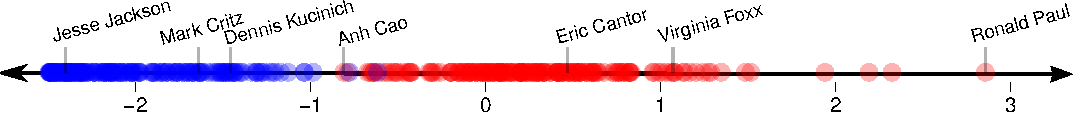
\includegraphics[width=0.95\textwidth]{chapter_spatial_voting_with_text/figures/3393_example_ideal_points_final.pdf}
  \caption{Example one-dimensional ideal points from the 111th House
  of Representatives.  Ideal points represent lawmakers' voting
  preferences. Democrats are blue and Republicans are red.}
  \label{figure:example_ideal_points}
\end{figure}

% dmb: i liked the section below about the utility model.  its
% interesting, but i propose we remove it or describe it in a
% paragraph somewhere else.  my reasoning is that its not essential to
% our story of ideal point-limitations-new model and, while elegant,
% its also complicated (i.e., introduces notation etc).  i want the
% reader to quickly understand ideal points and then start thinking
% about their limitations.  that said, i put a footnote about the
% utility model above.
% smg: got it.

% --- utility model begin ---



% \textbf{The Bayesian ideal point model.}
% The ideal point model is a generative model of choices (votes) and
% issues (bills).  Each legislator $u$ is associated with an
% \textit{ideal point} $X_u$ (see \myfig{ideal_points}), and each bill
% is associated with a \textit{discrimination} $B_d$ and
% \textit{difficulty} $A_d$.  The vote $v_{ud}$ is assumed drawn from the
% linear model
% \begin{equation}
%   \label{eq:ideal-point}
%   p(v_{ud} = \textrm{yea}) = \sigma(x_u b_d + a_d),
% \end{equation}
% where $\sigma(t) = \frac{\exp(t)}{1 + \exp(t)}$.  This is a logistic
% regression with random effects.\footnote{Some ideal point models use a
% probit model; we have found both approaches to ideal points to yield
% similar results}

% Notice the roles of the per-legislator and per-bill latent variables
% in \myeq{ideal-point}.  The difficulty parameter $a_d$ explains bills
% that all legislators will vote for or against, e.g., ``A bill to
% congratulate the winner of the World Series.''  For the remaining
% bills, i.e., those with some political division, the discrimination
% parameter $b_d$ and ideal point interact.  When estimated from roll
% call data, these latent variables capture the political leanings of
% the legislators and the political tone of the legislation.


\section{A model for predicting votes with the text of new bills}
%% Roll call data is essential for understanding government because it
%% represents atomic and concrete actions of its members.  But this data
%% is only one part of a richer record which includes bill texts,
%% speeches, press releases, public plans, and other items.  
 
In this section, we extend ideal point models to include other
information.  Specifically, we will use the text of bills to estimate
a bill's polarity and popularity.  This gives a new way of exploring
and analyzing the government record and, further, gives a useful
predictor of government.  While traditional methods can only fill in
missing votes, we develop tools that can predict how legislators will
vote on a new bill. This is the first work to study predictive
accuracy of votes on new bills, where we use a spatial voting model as
a ``cold'' prediction mechanism.

% \begin{figure}[t]
%   \includegraphics[width=0.45\textwidth]
%   {chapter_spatial_voting_with_text/figures/134_senator_name_accuracy_by_ip_sample.pdf}
%   \caption{Sample Senator ideal points in the 111th Congress.  Ideal
%     points tend to separate the U.S. political parties: Democrat are blue,
%     and Republicans are red. A plot of all legislators is included in
%     the supplementary materials.}
% \label{fig:ideal_points}
% %\vspace{-22pt}
% \end{figure}

% DMB-2011: sean, above, can you make a more readable figure of ideal
% points?  For example, you can just show the senators or show a
% subset of the representatives.  Give specifics in the paragraph (and
% caption) about which legislature is illustrated.
% SMG: I've gone from Senators-only to a subset of ~20 Senators.
% DMB-2011: above, we need a citation for the psychometrics model.
% SMG: Done.
As predictive models, ideal point models suffer from a
fundamental limitation: they are models of the votes alone.
Consequently, they can be used to fill in missing votes but cannot
predict how legislators will vote on future legislation.  Further,
they provide no insight into what drives voting patterns---the
political activity of the legislature is summarized with two columns
of real numbers.

To these ends, we will describe several models that connect the voting
patterns of legislators to the original text of bills.  One of these
models embeds the statistical assumptions of \textit{supervised topic
  modeling}~\cite{blei:2008} into the ideal point model, where the
locations of the bills are predicted from the latent topics in their
texts. This model---the ideal point topic model---can predict complete
votes on pending bills and provides a new way of exploring how
legislative language is correlated with political support.  The other
models predict inferred ideal points using different forms of
regression on phrase counts.

In the following sections, we review the details of ideal point
estimation and develop several models for predicting votes from
legislative text.  We derive an approximate posterior inference
algorithm for ideal point models based on variational methods and
analyze six Congresses (12 years) of legislative data from the United
States Congress.  Given a legislative history, these models can
accurately predict votes on future legislation.  One of these models,
the ideal point topic model, can help summarize and visualize the
political landscape of a government body based both on the voting
patterns of its members and the language of its issues.

\begin{figure}[t]
\center
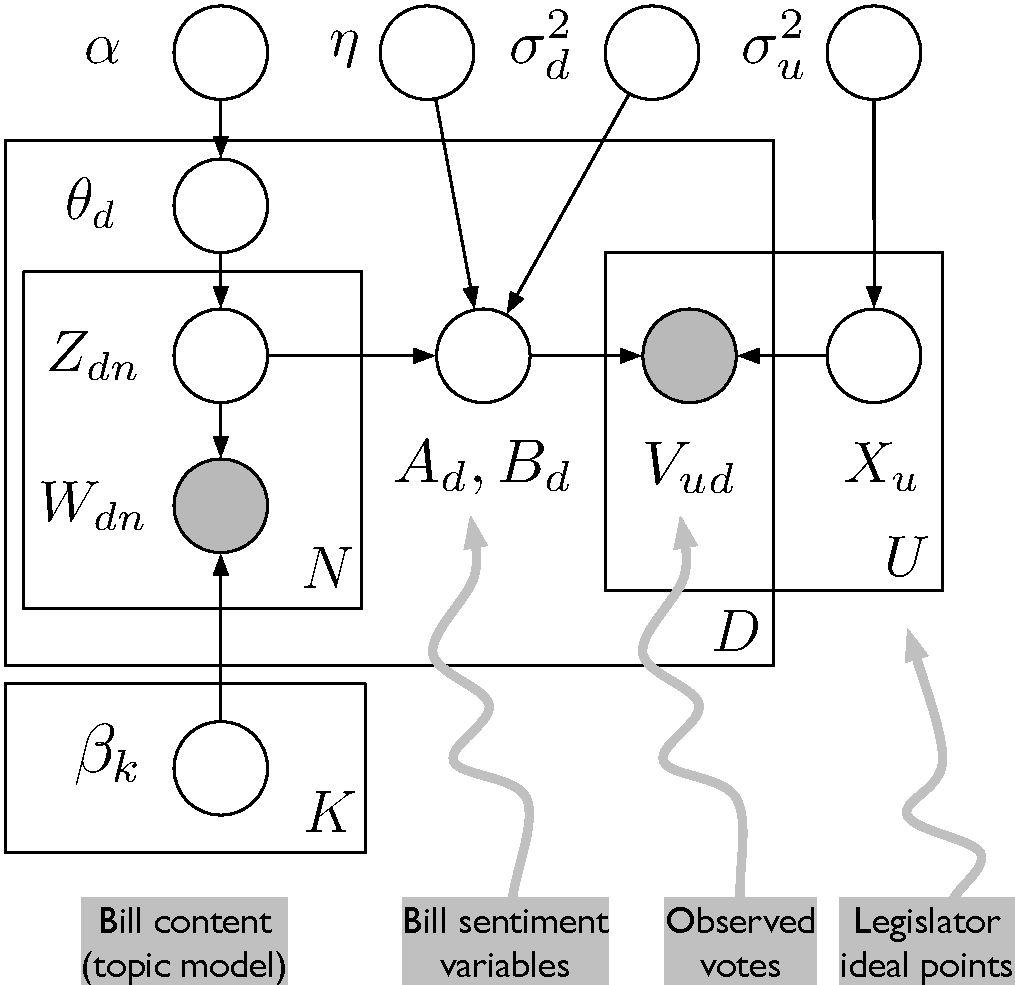
\includegraphics[width=0.5\textwidth]{chapter_spatial_voting_with_text/figures/ideal-point-topic-model.pdf}
\caption{The ideal point topic model.  Priors over the multinomials
$\theta_d$ and $\beta$ are both symmetric Dirichlet distributions.}
\label{fig:legis_gm}
\end{figure}

We now develop models relating the text of a bill to the variables
$a_d$ and $b_d$.  Associating text to bill variables has a predictive
advantage because new bills can be situated in the space of ideal
points.  It also has an interpretive advantage because language
becomes associated with political sentiment.

\textbf{Modeling ideal points with text regression.} We developed two
predictive ideal-point models which use text
regression~\cite{Kogan:2009}.  For these, we first fit an ideal-point
model to a training set of bills and all legislators using the
variational algorithm described in \mysec{model}.  We then fit ridge
regression\footnote{Implemented in the ``penalized'' package for R}
(\verb!LARS!) and Lasso
\footnote{implemented with the ``lars'' package for R} (\verb!L2!) to
these bills' parameters $a_d, b_d$ using a vector of their
$n$-gram\footnote{See \mysec{experiments} for details.}  counts $\bm
w_{d}$ as covariates.

\textbf{Modeling ideal points with supervised topics.} The text
regression models link individual words or phrases to bill sentiment.
In this section, we connect textual \emph{themes} with bill sentiment.
We refer to this model as an ideal point topic model (IPTM).

To model themes, we use the assumptions of supervised Latent Dirichlet
Allocation (sLDA)~\cite{blei:2008}.  As in Latent Dirichlet Allocation
\cite{blei:2003}, each bill is represented as a mixture of latent
topics $\theta_d$, where each of $K$ topics $\beta_k$ is a multinomial
probability distribution over terms.  For the $n^{th}$ term of bill
$d$, we draw topic $z_{dn}$ from $\mbox{Mult}(\theta_d)$, and then
draw word $w_{dn}$ from the topic $\beta_{z_n}$.

% the Dirichlet prior for $\theta$ has parameter $\alpha$.

% DMB-2011: above, that point can be mentioned in the caption of the
% graphical model.  (that caption should summarize the rest of the
% notation too.  it's a good place for that.)

% DMB-2011: it also looks like we need to add the dirichlet prior on topics
% to the graphical model.

Like sLDA, the ideal point topic model further assumes each bill
$d$ is attached to a response variable.  In this case, the
response variable is the 2-component vector of bill variables $(a_d,
b_d)$.  The distribution of the response is a linear model whose
covariates are the empirical distribution of the topics $\bm z_d$ for the
bill,
\begin{eqnarray*}
  a_d &\sim& {\cal N}(\bm \eta_a^\top \bm \bar{z}_d, \sigma_d^2) \nonumber \\
  b_d &\sim& {\cal N}(\bm \eta_b^\top \bm \bar{z}_d, \sigma_d^2), \nonumber \\
\end{eqnarray*}
where $\bar{z}_d = (1/N) \sum_n z_{dn}$.  This setting is more complex
than the original sLDA model: the response variables are
\textit{hidden}---they are not observed directly, but are used
downstream in the voting model.

Finally, we add a Gaussian prior to $\bm \eta$.  The full model is
represented as a graphical model in \myfig{legis_gm}.

The only observed variables in the model are the bill texts and votes.
Our goal in fitting this model is to uncover the posterior
\begin{equation}
  p(a_d, b_d, x_u, \bm \eta, \beta, z, \theta | \bm W, \bm V), \label{eq:posterior}
\end{equation}
which can then be used in exploratory or predictive tasks.
Conditioned on these variables, our analysis proceeds with the
posterior distribution of the ideal points, polarities and
difficuties, topics, and coefficients. Computing the posterior exactly
is intractable, so we use variational inference to approximate it.  We
describe this in further detail in \mysec{inference}.

% DMB-2011: insert notation of the posterior here; just the LHS p(
% blah given blah).  it looks like something along the lines of the
% first paragraph of the inference section might do the trick.  then,
% in the inference section, just recall these tasks (and equations)
% and get right to why its difficult to actually do them.  (in fact,
% you can even mention that here too and forward point to the section
% on computation.)

% DMB-2011: outline the process of prediction above SMG: Prediction
% details were originally explained in the variational inference
% section.  I think it makes sense to leave them there, since we don't
% have variational parameters defined yet.
This posterior allows us to explore the connection between language
and political tone.  For example, the coefficients $\bm \eta$ are a
direct connection between bills' topics and the political tone of
these bills. Examples of this are provided in \mysec{experiments}.
The topics $\beta$, learned from both text and votes, provide a
lexical window into legislative issues.  The parameters $\bm \eta,
\beta$ together also allow us to predict votes using the text of new
bills; \mysec{inference} provides detail about this.

% DMB-2011: finish above too.  the idea is that the coefficients &
% topics together tell us how the model has associated language with
% discrimination or difficulty.  maybe forward point to some examples.

% The full likelihood of this model is given by
% \begin{eqnarray}
% \label{likelihood}
%   p(\bm W, \bm V, W, z, I, X, \theta, \bm \eta) = \nonumber \\
% & \hspace{-90pt} \prod_D  p(\theta_d | \alpha) \prod_N p(w_n | z_n, \beta)
%    p(z_n | \theta_d) \nonumber \\
% & \hspace{-90pt} \times \prod_D p(I_d | z_{d, 1:n}, \bm \eta) \times p(\bm \eta) \nonumber \\
% & \hspace{-90pt} \times \prod_U p(x_u) \prod_D p(v_{ud} | x_u, I_d). \nonumber \\
% \end{eqnarray}
% This likelihood is also represented in the graphical model in

%A. Ideal point model - we use logit, jackman, quinn use MCMC.  The
%results in \mysec{ideal} suggest that the results are very
%similar.

%  B. Supervised topics C. Full Likelihood function

\subsubsection*{Multimodal solutions and identification}
Note that a fit of the ideal point model has multiple modes.  In one
mode, Democrats tend to have positive ideal points, while Republicans
are negative; in another, Republicans are positive, while Democrats
are negative.  To keep fits of the different models identifiable,
several researchers have applied nonzero priors over specific
legislators to encourage the model to prefer one of these modes
\cite{jackman:2001,clinton:2004,martin:2002}.

In the study in \mysec{experiments}, we anchor four legislators with
strong priors ($\sigma_d = 10^{-3}$) at ideal points $\pm 4$.  We
select two congresspersons from each chamber and two from each party:
Kennedy (S-Dem) and Waxman (H-Dem) are centered at +4 and Enzi (S-Rep)
and Donald Young (H-Rep) are centered at -4.\footnote{This value was
selected to be large yet not completely out of the ordinary.} We
selected these Senators for consistency with previous
work~\cite{clinton:2004}.  We selected the Representatives because
they have held long offices in the House.  Without these sharp priors,
the model still discovers ideal points which cleanly separate
political parties but may converge on ``opposite'' modes in different
fits.  With the priors, we obtain consistent ideal points at the
expense of predictive performance.

\subsection*{Related work}

% Spatial voting models begin with a strong assumption about what
% causes individuals (often voting citizens) to vote as they
% do~\cite{enelow:1984}.
% % TODO(sgerrish): contrast these with other models of voting.

Ideal point models, a form of spatial voting model, have roots as far
back as the 1920s \cite{enelow:1984}. They are fit by both
frequentist~\cite{poole:1985,heckman:1996} and Bayesian
methods~\cite{jackman:2001,martin:2002,clinton:2004}, have been
embedded in a time series~\cite{martin:2002,wang:2010}, and have been
developed for higher dimensional political
spaces~\cite{jackman:2001,heckman:1996}.

% \nocite{jackman:2001}
\nocite{johnson:1999ch6}

Topic models have been applied to Senate speeches, such as to discern
``the substantive structure of the rhetorical [legislative] agenda''
\cite{quinn:2006}.  They have also been used with legislative speeches
to gauge legislators' sentiment toward legislation using roll-calls
\cite{thomas:2006}.  Modeling sentiment in text is more generally
discussed in the field of sentiment analysis; see Pang and Lee
\cite{pang:2008} for a review.

% DMB-2011: the above explanation is confusing.  how is a document
% drawn from a mixture of gaussians?  are there topics in their model?
% SMG: Clarified.

The ideal point topic model relates closely to user-recommendation
models based on matrix factorization~\cite{Salakhutdinov:2008a}.
Matrix factorization methods for recommendation are akin to
large-scale spatial behavior models (though usually with no
``difficulty'' term, which acts as an intercept).  Many of these
matrix factorization models for user recommendation do not provide a
method of predicting one user's item preference without other users'
preferences on the same item.

Two works stand out as closely related to this work.  One of these is
fLDA, which models binary or continuous ratings with user affinity to
topics \cite{agarwal:2010}.  Another is Wang et
al. \cite{wang:2010}, who describe a similar application by
combinating topic models and matrix completion.  Their work also draws
on ideal point models, models transitions over time, and is designed
to learn the dimensionality of the latent factors.  Under the
generative assumptions of their model, bills and matrix cells (e.g.,
votes) are conditioned on a shared mixture; in our model, votes are
conditioned on words' topics.

% \cite{poole:1985} Present a spatial model for analyzing
%roll-calls.

% - poole and rosenthol K. T. Poole and H. Rosenthal.  ``A Spatial
% Model for Legislative Roll Call Analysis.''  American Journal of
% Political Science, Vol 29 (1985a), pp. 356-384 - present NOMINATE.
% Is a \cite{heckman:1996} Present a linear probability model known as
% NOMINATE.  Application to roll-call analysis.


% \cite{johnson:1999ch6} Provides discussion of Bayesian inference and
% model checking for item-response models.  Johnson (ch. 6) notes
% Early analysis of item response models are found in Swaminathan and
% Gifford (1982, 1985) and Tsutakawa and Lin (1986).  Patz and Junker
% (1997) demonstrate Metropolis within Gibbs simulation for Bayesian
% Item Response models with Logistic link.

% heckman: probabilistic models for inferring votes - linear
% probability model of preferences motivated by rational choice theory
% for economics - uses an ideal point, or ``bliss point'' -
% justification: taylor approximation of utility - factor-analytic
% model (according to jackman) - produces consistent estimates - find
% at least 6 statistically significant dimensions - model goods:
% computational simplicity, ability to rigorously estimate dim.

% - enelow and hinich: euclidean spacial voting model (1984) ``The
% Spatial Theory of Voting: an Introduction'' 1984 J. Enelow and
% M. Hinich Cambridge University Press.  New York.

% K. T. Poole and H. Rosenthal.  ``Analysis of Congressional Coalition
% Patterns: A Unidimensionaal Spatial Model.''  American Journal of
% Political Science, Vol 29 (1985a), pp. 356-384 Spatial Models of
% Legislative Voting, Keith T. Poole.  - in 1997 present D-NOMINATE.
% - nonlinear probability model - assume logistic model of

% - Rabinowitz and McDonald: directed preference model (1989)

% - gorman

%    W-nominate is normal-logit
%    NOMINATE
%     - max-likelihood estimation.  does not produce consistent estimates.


%  B. Ideal point models
%    - jackman, clinton take Bayesian approach, to take advantage of
%    the MCMC sampling machinery for inference, and to make inferences and
%    substantive hypotheses about ideal points.

%    - in addition, Jackman notes that the methodology can provide a coherent framework of hypothesis testing \cite{gelman:1996}
%    - compare this approach with

%%% Local Variables:
%%% mode: latex
%%% TeX-master: "icml2011"
%%% End:

\subsection*{Posterior estimation for the ideal point topic model}
\label{sec:inference}
Computing the posterior in \myeq{posterior} is intractable.  Posterior
inference for traditional Bayesian ideal point models is traditionally
implemented with MCMC methods such as Gibbs sampling
\cite{johnson:1999ch6,jackman:2001,martin:2002,clinton:2004}.
However, in the ideal point topic model, fast Gibbs samplers are
unavailable because the conditionals needed are not analytically
computable; an MCMC strategy would require a more complicated sampling
scheme. We therefore use an alternative algorithm -- which can be applied
to both the standard ideal point model and the ideal point topic model
-- which uses variational methods \cite{jordan:1999}.

Recall from Chapters 2 and 3 that to variational inference requires
specification of a variational distribution which will serve as a
proxy for the true posterior.
% dmb: make it clear that we use a fully-factorized variational
% distribution.
% smg: added a note below.  We use a fully-factorized variational
distribution.  Word assignments $z_{dn}$ and topic proportions
are governed by multinomial parameters $\phi_d$ and Dirichlet
parameters $\gamma_d$, as in LDA~\cite{blei:2003}.  The variational
distribution for legislators' ideal points $x_u$; bills' parameters
$a_d, b_d$; and coefficients $\bm \eta$ are Gaussian with respective
means $\tau_u$, $\kappa_d$, $\ev$ and variances $\sigma_\tau^2$,
$\sigma_\kappa^2$, $\sigma_\eta^2$. The variational distribution is
\begin{align}
\label{eq:var_post}
q(\tau, & \sigma_\tau, \kappa, \sigma_\kappa, \phi, \theta) = \\
& \prod_u q(x_u | \tau_u, \sigma_\tau^2 ) \times \prod_D q(a_d, b_d |
\kappa_d, \sigma_\kappa^2 ) & \nonumber \\
\textstyle & \times \prod_D q(\theta_d | \gamma_d) \prod_{N_d} p(z_n |
\phi_n) \times q(\bm \eta | \ev, \sigma_{\ev}). \nonumber
\end{align}

Inference proceeds by minimizing the KL between \myeq{var_post} and
the true posterior \ref{eq:posterior}, which is equivalent to
maximizing a lower bound on the marginal probability of the
observations.  Coordinate ascent only works for some of the random
variables, but we must use gradient ascent on $a_d, b_d,$ and $x_u$.
The supplementary materials give further details of the variational
inference algorithm.

\textbf{Prediction} After they are fit to legislators' votes and bill
text, the variational parameters $\tau$, $\ev$, and $\beta$ can be
used to estimate the vote of each legislator on a \emph{new} bill $d$
using its text.  To predict whether legislator $u$ votes \verb!yea! on
$d$, the per-word parameters $\phi_n$ of $d$ are estimated using the
topics $\beta$. Once $\phi$ has been estimated, the probability of a
\verb!yea! vote is given by $p(v_{ud} = \verb!yea!)  = \sigma(\tau_u
(\bar{\phi_d} \ev_b) + \bar{\phi_d} \ev_a)$
\footnote{The estimate $\expectq{\sigma(x_u (\bar{z_d} \eta_b) +
    \bar{z_d} \eta_a)}$ can be more theoretically justified, but
  results from the two estimates are (in practice) identical.}, where
$\bar{\phi_d}$ is $\frac{1}{N_d} \sum_{N_d} \phi_n$.  In practice, we
fit $\ev$ with no regularization after the model has converged.  This
gives slightly better results which are more robust to parameter
selection.

\subsection*{An empirical analysis}

\begin{figure}
\label{fig:log_likelihood}
\begin{center}
  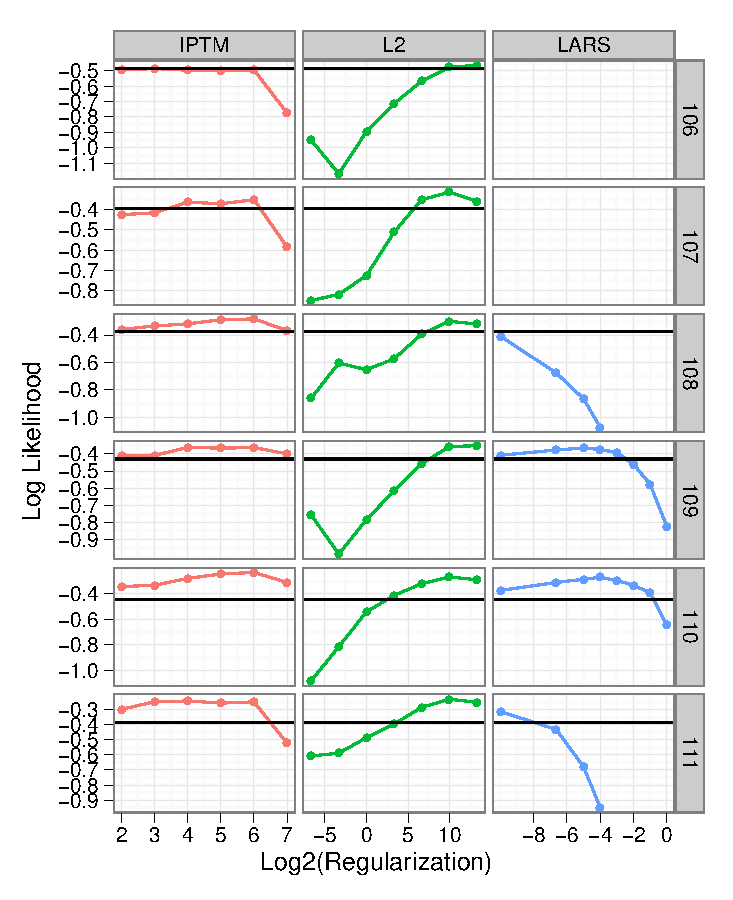
\includegraphics[width=0.9\textwidth]
{chapter_spatial_voting_with_text/figures/138_log_likelihood_by_session_topics.pdf}
\end{center}
\vspace{-6pt}
\caption{Vote log likelihood on heldout votes. Models are shown
  by color for different regularizations (x axis), for Congresses 106
  to 111.  For LARS and L2, the regularization is the complexity
  parameter; for the ITPM, the regularization is the the number of
  topics.  The \emph{yea} baseline is the horizontal black line. LARS
  is below the fold for 106-107.  The ideal point topic model performs
  with less variance across its regularization parameter. }
\vspace{-3pt}
\end{figure}
\subsubsection*{Analyzing the U.S. House and Senate}
\label{sec:experiments}

We studied the performance of these models on 12 years of data from
the United States House of Representatives and Senate.  We first
demonstrate how the ideal point topic model can be used to explore
legislative data; then we evaluate the models' generalization
performance in predicting votes from bill texts.

We collected roll-coll votes for Congressional sessions 106 through
111 (January 1997 to January 2011).  We used votes about bills and
resolutions, and only votes regarding the legislation as a whole
(as opposed to, e.g., amendments of the legislation). We downloaded
the data from Govtrack, an independent Website which provides
comprehensive legislative information to the public.  Our
collection contains 4,447 bills, 1,269 unique legislators, and
1,837,033 \verb!yea! or \verb!nay! roll-call votes.

To select the vocabulary, we lemmatized the bills with
Treetagger~\cite{treetagger}.  Then we retained a vocabulary of
statistically significant $n$-grams ($1 \le n \le 5$) using likelihood
ratios.  These $n$-grams were treated as terms.\footnote{When one
  $n$-gram subsumes another, we chose to observe the longer of the
  two}  We removed $n$-grams occurring in fewer than 0.2\% of all
bills and more than 15\% of bills.  We also removed an
$n$-gram if it accounted for more than 0.2\% of all tokens or fewer
than than 0.001\% of all tokens.  After this process, our vocabulary
contained 4,743 unique $n$-grams.

We used the anchor legislators described in \mysec{model}.  We ran
variational inference until the change in increase in the objective
function was less than 0.01\%.

\subsubsection*{Exploring topics and bills}

In this section, we examine a fit of the ideal point topic model for
all the bills and votes of a session.  This demonstrates the model's
use as an exploratory tool of political data.  For this analysis, we
used dispersion $\sigma_d = \sigma_u = 1.0$ and 64 topics.  We focus
on the $111^{th}$ session (January 2009 to January 2011).

\textbf{Exploring topics with $\ev$.} As noted in \mysec{model}, the
coefficients $\ev$ relate each topic's weight in a bill with the
bill's difficulty and polarity parameters. \myfig{topics} shows
some example topics and their corresponding coefficients $\ev$.  Below
we describe some of these topics in more detail and connect them to
the data.

\begin{figure}
  \center
  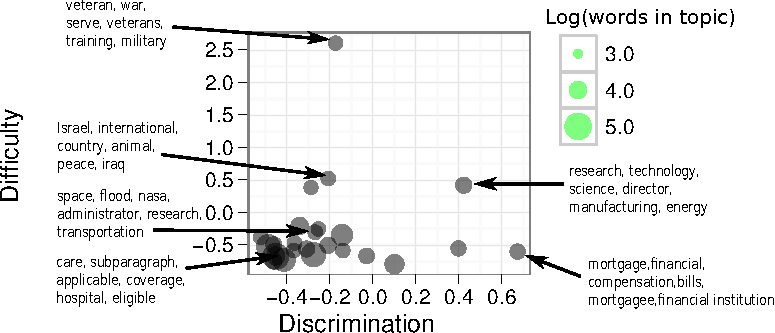
\includegraphics[width=0.9\textwidth]{chapter_spatial_voting_with_text/figures/134_64_topic_plot.pdf}
  \caption{Topics can be visualized in the same latent political space
    as legislators and bills.  This plot shows selected topics by
    coefficients $\ev$, for a 64-topic model ($\ev$s are normalized by
    mean and variance).  Two topics (\emph{people, month, recognize, ...}
    and \emph{clause, motion, chair, ...}) with difficulty 4.68 and
    polarity 7.4 (respectively) are not shown.}
  \label{fig:topics}
\end{figure}

One popular topic in the 111th Congress focused on national
recognition: \emph{people, month, recognize, history, week, woman}.
In contrast, the \emph{least}-supported topic was more procedural,
frequently appearing in bills under consideration or with many
amendments (\emph{clause, motion, chair, print, offer, read}).  In
this case, such legislation is sometimes summarily rejected before
further consideration; the language of amendments is a signal that
legislation is contentious.

While these topics often explained overwhelming support or rejection
of legislation, much legislation was considerably more partisan.

\textbf{Health Care.}  One contentious topic was about
% parameters: Discrimination 0.122, Difficulty 4.75
qualification for public health care: \emph{care, subparagraph,
applicable, coverage, hospital, eligible}.  This topic was among the
most-Democratic 10\% of topics, in large part because it helped to
explain the \emph{Patient Protection and Affordable Care Act},
i.e. the ``Health Care Bill'' of 2009.  Although this 906-page bill
was barely passed: of the 311 Democrats voting on
it, 276 voted in favor; of the 217 Republicans voting on it, none
voted in favor.  The model was moderately accurate on this bill: it
correctly predicted 93.8\% of votes.  The two other topics highly
expressed in this bill were about different aspects of public health,
including one about government health options (medicare and social
security) and one about health insurance coverage; both were slightly
Democratic.

\textbf{NASA Authorization.}
Another contentious topic was about spaceflight: \emph{space, flood,
NASA, administrator, research, transportation}.
This topic was expressed in one of the most-poorly predicted bills of
the $111^{th}$ Congress.  This bill, the \emph{NASA Authorization Act
of 2010}, was a "compromise between the Obama administration, which
wants... a commercial space industry in which private companies would
transport astronauts, and House lawmakers, who wanted... one
government-owned rocket" \cite{herszenhorn:2010}.  In the house vote
(a Senate record was not kept), of 249 Democrats voting on the bill,
185 voted in favor; of the 173 Republicans, 119 voted in favor.
Because this bill had mixed but nonpartisan support, the model could
not represent it well, with only 72\% of votes correctly predicted.

\subsubsection*{Checking the ideal points}
We can also use the in-sample fit to assess the quality of the ideal
points of the legislators.  In classical ideal point modeling, this is
done via in-sample accuracy: How well does the model explain the
observed votes?

The average per-legislator accuracy in the in-sample fit was 96\%
(only 10\% of legislators had accuracy lower than 90\%).  As expected,
accuracy increases with more votes ($\rho=0.51$).  Among legislators
with over 100 votes, only two stand out. Donald Young (713 votes;
accuracy 0.83) had a pre-defined ideal point (see \mysec{model}). Ron
Paul, a Republican in the $111^{th}$ Congress, was also poorly
predicted (761 votes; accuracy 0.84).  Paul is known for his
Libertarian beliefs, even having run for President for the Libertarian
party in 1988.

The poor prediction of Paul points to a limitation of the
1-dimensional ideal-point model, which can only capture the two main
parties, instead of a limitation of the supervised prediction: fitting
votes to the classical ideal point model (ignoring bill text), Paul's
in-sample accuracy was consistently poor across sessions.

\subsubsection*{Predicting votes from text}

\textbf{Prediction on heldout bills.}  We measured predictive accuracy
and log likelihood for these models under a variety of regularization
settings (\verb!LARS! is parameterized by $0 < f \le 1$, \verb!L2! is
parameterized by $\Lambda \ge 0$, and \verb!IPTM! is parameterized by
topics $K$).

We also devised two baselines for comparison with the three models
described so far.  The first of these provides a lower bound: assume
all votes are \verb!yea!.  Because the majority (85\%) of votes in our
corpus were \verb!yea! votes, this presents a more reasonable overall
baseline than random guessing (at 50\%).  We call this model the
\verb!yea!  model.  The second baseline fit a logistic regression
trained for members of each party (with a separate one for mixed or
independent legislators), with terms as covariates.  This baseline
(implemented with the R \verb!glm! library) used too much memory to
use more than 800 terms and therefore led to results worse than the
\verb!yea!  baseline.

For each 2-year period (called a Congress), the bills were partitioned
into 6 folds.  For each model, we iteratively (1) remove a fold, (2)
fit the model to the remaining folds (by Congress), and (3) form
predictions on the bills in the removed fold.  Across folds, we thus
obtain a complete data set of held-out votes.

Across all sessions, the \verb!yea! baseline predicts votes correctly
85\% of the time.  The ideal point topic model is better, correctly
predicting 89\% of votes with 64 topics (this means that 62,000 more
votes are correctly predicted).  Overall performance for \verb!L2! was
best for $\Lambda=1000$ (90\%), and \verb!LARS! was best at $f=0.01$
(82\%).  While the ideal point topic model had lower accuracy than
\verb!L2!, its log-likelihood was nearly the same.  These results are
summarized in \myfig{log_likelihood}, and further details are in the
supplementary materials.

\textbf{Sequential prediction.}  Our final study examined the
performance of these models on predicting future votes from past
votes.  To do this, we fit a 64-topic \verb!IPTM! and \verb!L2!
predictive models on the first $3, 6, 9, \ldots, 21$ months of a
Congress.\footnote{A bug prevented LARS from completing in most runs of
this setting}  We then tested these each of these fits on the
following three months of unseen votes.  The ideal-point topic model
correctly predicted $87.0\%$ of votes, and \verb!L2!  correctly
predicted 88.1\% of votes; their log-likelihood was identical.

With these models, one could predict 31,000 to 55,000 votes
above the baseline, \emph{based only on the text of the bills}.  The
simpler of the two models, \verb!L2!, performs better at prediction.

\section{Lawmakers' issue preferences in the U.S. Congress}

We now move on to  TODO(sgerrish): finish.

But there are some votes that ideal point models fail to capture.  For
example, Ronald Paul, Republican representative from Texas, and Dennis
Kucinich, Democratic representative from Ohio, are poorly modeled by
ideal points because they diverge from the left-right spectrum on
issues like foreign policy. Because some lawmakers deviate from their
party on certain substantive issues, their positions on these issues
are not captured by ideal point models.

% dmb: give examples above
%
% Paul's views on foreign policy are more left-wing than expected.
% Kucinich's views on on

%% The broader issue is that the ideal points place each lawmaker
%% in a single position.  In real data, lawmakers take positions on
%% issues, such as foreign policy, environmental problems, and social
%% welfare.  A lawmaker's vote on a bill has to do with his political
%% affiliation, the content of the bill, and his position on that
%% content.  Traditional ideal point models do not take issues into
%% account.

%Ron Paul's views on foreign policy
%could be inferred by inspecting lawmakers close to him in this latent
%space $\mathbb{R}^p$,

To this end, we develop the \emph{issue-adjusted ideal point model}, a
latent variable model of roll-call data that accounts for the contents
of the bills that lawmakers are voting on.  The idea is that each
lawmaker has both a general position and a sparse set of position
adjustments, one for each issue.  The votes on a bill depend on a
lawmaker's position, \emph{adjusted} for the bill's content.  The text
of the bill encodes the issues it discusses. Our model can be used as
an exploratory tool for identifying exceptional voting patterns of
individual legislators, and it provides a richer description of
lawmakers' voting behavior than the models traditionally used in
political science.

% Our goal in this work is to introduce a latent-variable model that
% uses thematic labels for legislative items to describe lawmakers'
% positions on different issues.  We do this with a sparse
% representation of each lawmaker's unique voting behavior.  With this
% approach, we circumvent manual interpretation of dimensions by
% explicitly labeling bills with issue weights.  

In the following sections, we develop our model and describe an
approximate posterior inference algorithm based on variational
methods.  We analyze six Congresses (12 years) of legislative data
from the United States Congress.  We finally show that our model gives
a better fit to legislative data and provides an interesting
exploratory tool for analyzing legislative behavior.

\subsection{A model of exceptional voting patterns}
%\pagecolor{yellow}
\label{section:exceptional_model}

\subsubsection{Limitations of ideal point models.}

A one-dimensional ideal point model fit to the House of
Representatives from 2009-2010 correctly models 98\% of all lawmakers'
votes on training data. But it only captures 83.3\% of Baron Hill's
(D-IN) votes and 80.0\% of Ronald Paul's (R-TX) votes.  Why is this?

The ideal point model assumes that lawmakers are ordered.  Each bill
$d$ splits them at a \emph{cut point} $-\frac{b_d}{a_d}$.  Lawmakers
to one side of the cut point are more likely to support the bill, and
lawmakers to the other side are likely to reject it.  For lawmakers
like Paul and Hill, this assumption is too strong because
their voting behavior does not fit neatly into a single ordering.
Their location among the other lawmakers changes with different bills.
% \begin{figure}
%   \begin{center}
%     \vspace{-10pt}
%     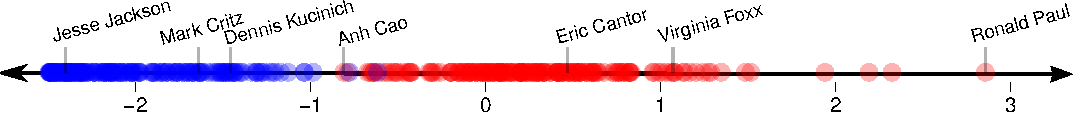
\includegraphics[width=0.8\textwidth,height=0.1\textwidth]{chapter_spatial_voting_with_text/figures/3393_example_ideal_points_final.pdf}
%     \vspace{-10pt}
%   \end{center}
%   \caption{Traditional ideal points separate Republicans (red) from Democrats (blue).}
%   \label{fig:classic_ideal_points}
%   \vspace{-5pt}
% \end{figure}

\begin{figure}
  \center
  \begin{tabular}{c}
  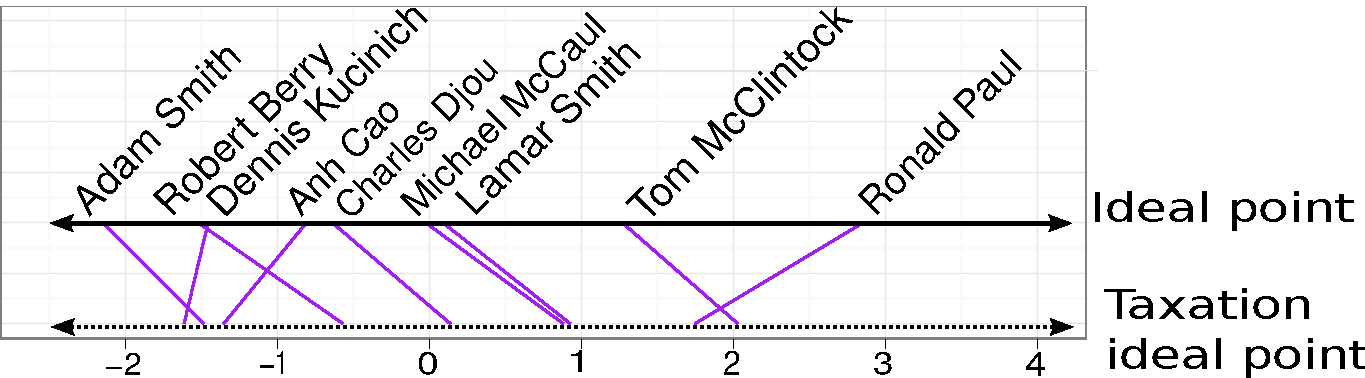
\includegraphics[width=0.75\textwidth]{chapter_spatial_voting_with_text/figures/3393_example_ideal_points_taxation.pdf} \\
  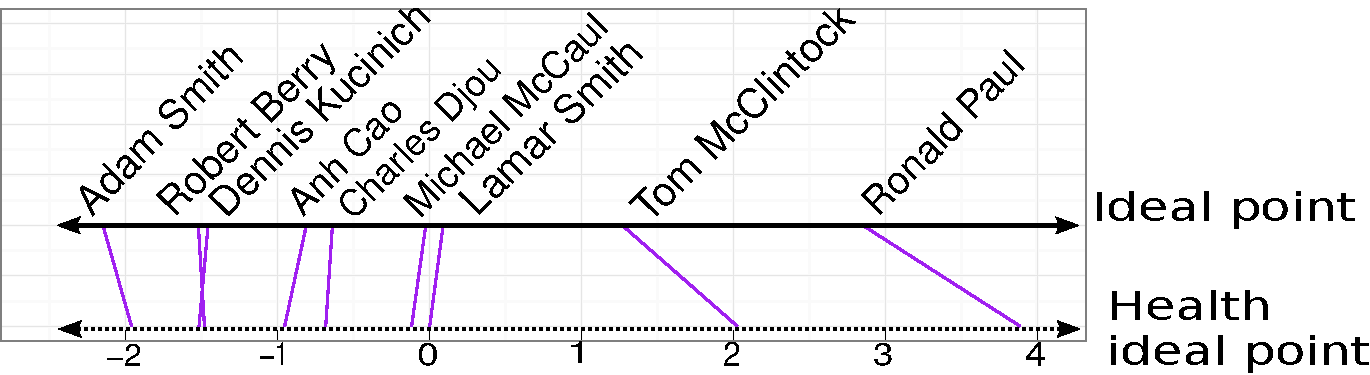
\includegraphics[width=0.75\textwidth]{chapter_spatial_voting_with_text/figures/3393_example_ideal_points_health.pdf} \\
  \end{tabular}
  \caption{In a traditional ideal point model, lawmakers' ideal points
    are static (top line of each figure).  In the issue-adjusted ideal point model, lawmakers'
    ideal points change when they vote on certain issues, such as
    \emph{Taxation} (top) and \emph{Health} (bottom).}
  \label{fig:moving_ideal_points}
\end{figure}

Lawmakers do not vote randomly, however.  They vote consistently
within individual areas of policy, such as foreign policy and
education.  Paul consistently votes against United States involvement
in foreign military engagements, a position that contrasts with other
Republicans.  Democratic representatives from New York are more likely
to hold conservative positions on financial services regulation, even
though they vote Democratically on social issues.

We refer to voting behavior like this as \emph{issue voting}.  An
\emph{issue} is any federal policy area, such as ``financial
regulation,'' ``foreign policy,'' ``civil liberties,'' or
``education,'' on which lawmakers are expected to take positions.
Lawmakers' positions on these issues will often diverge from their
traditional left/right stances.  The model we will develop captures
this, as illustrated in Figure~\ref{fig:moving_ideal_points}; for
example, Charles Djou is more similar to Republicans on
\emph{Taxation} (right) and more similar to Democrats on \emph{Health}
(left), while Ronald Paul is more Republican-leaning on \emph{Health}
and less extreme on \emph{Taxation}. The model we will introduce uses
lawmakers' votes and the text of bills to model deviations like this,
on a variety of issues.

% dmb: move this to later.  i think this is done.

% In the model we develop below, we assume that lawmakers have a
% separate position for each issue.  Their votes for legislation about
% an issue are determined by these positions.

% dmb: this point should be made in the modeling section, somewhere.
% in fact, let's put a graphical model somewhere and write this near
% it.
% smg: done

% Said differently, lawmakers' votes on bills are conditionally
% independent given their position on the issues.

\subsubsection{Issue-adjusted ideal points.}

% dmb: we made these points above

% The problem with traditional ideal point models is that unidimensional
% ideal points are too constrained, while multidimensional ideal points
% are hard to interpret absent painstaking substantive study.  Our goal
% is to create a model of lawmakers' issue-voting behavior by using
% explicitly labeled issues. Assuming a mixture $\bm \theta_d \in [0,
% 1]^K$ (with $\sum_{k=1}^K \theta_{d,k} = 1),$ of issues attached to
% each document, this motivates a tentative model of the form

We now describe a new model of lawmaker behavior that takes into
account both the content of the bills and the voting patterns of the
lawmakers.  We build on the ideal point model so that
each lawmaker's ideal point can be adjusted for each issue.

%\begin{wrapfigure}{r}{0.5\textwidth}
\begin{figure}
  \center
  \begin{tabular}{cc}
    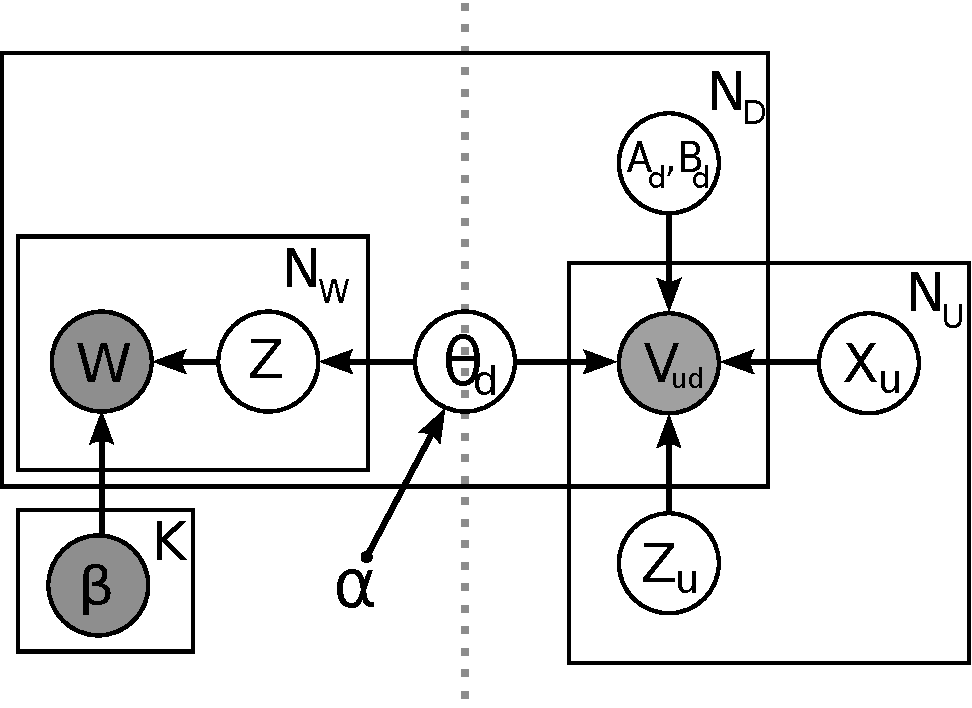
\includegraphics[width=0.4\textwidth]{chapter_spatial_voting_with_text/figures/legis_gm.pdf} &
%%  \begin{tabular}{c\begin{tabular}{|c|c|c|c|}
%%     \hline
%%     \textbf{Terrorism} &
%%     \textbf{Commemorations} &
%%     \textbf{Transportation} &
%%     \textbf{Education} \\
%%     \hline
%%     terrorist & nation & transportation & student \\
%%     september & people & minor & school \\
%%     attack & life & print & university \\
%%     nation & world & tax & charter school \\
%%     york & serve & land & history \\
%%     terrorist attack & percent & guard & nation \\
%%     hezbolah & community & coast guard & child \\ 
%%     national guard & family & substitute & college \\    
    \small
 \begin{tabular}{c}
 \begin{tabular}{|cc|cc|}
    \hline
    \multicolumn{2}{|c|}{\textbf{Terrorism}} & \multicolumn{2}{|c|}{\textbf{Commemorations}} \\
    \hline
    terrorist & york & nation & serve \\
    September & terrorist attack & people & percent \\
    attack & Hezbollah & life & community \\
    nation & national guard & world & family \\
    \hline
  \end{tabular} \\
  \begin{tabular}{|cc|cc|}
    \hline
    \multicolumn{2}{|c|}{\textbf{Education}} & \multicolumn{2}{|c|}{\textbf{Transportation}}  \\
    \hline
    student & history & transportation & land \\
    school & nation & minor & coast guard \\
    university & child & print & substitute \\
    charter school & college & tax & nature \\
    \hline
  \end{tabular}
 \vspace{110pt}
\end{tabular}
        \vspace{-100pt}
 \\
 \normalsize
%  \textbf{Labeled topics} \\
%% \vspace{40pt}
%   \begin{tabular}{|cccc|}
%%     \hline
%%     student      & transportation & intelligence & states \\
%%     school       & highway        & states       & postal service \\
%%     institution  & safety         & director     & fcc \\
%%     teacher      & vehicle        & personnel    & post office \\
%%     training     & states         & inspector    & network \\
%%     educational  & bridge          & officer     & internet \\
%%     award        & research       & terrorism    & computer \\
%%     academic     & rail           & foreign      & carrier \\
%%     \hline
%%  \end{tabular} \\
%%  \textbf{Unsupervised topics (standard LDA)}
%
%  \label{table:example_topics}
%\end{table}
        The issue-adjusted ideal point model & Labeled topics \\
    \end{tabular}
  \caption{Left: the issue-adjusted ideal point model, which models votes
    $v_{ud}$ from lawmakers and legislative items.  Classic item
    response theory models votes $v$ using $x_u$ and $a_d, b_d$.
    For our work, documents' issue vectors $\bm \theta$ were estimated fit with a topic
    model (left of dashed line) using bills' words $w$ and labeled topics
    $\beta$.  Expected issue vectors $\expectq{\bm \theta | \bm w}$ are then treated as constants
    in the issue model (right of dashed line).
  Right: Top words from topics fit using labeled LDA \cite{ramage:2009}.
  }
  \vspace{-5pt}
  \label{figure:legis_gm}
  \label{table:example_topics}
\end{figure}
%\end{wrapfigure}
Suppose that there are $K$ issues in the political landscape.  We will
use the words $\bm w_d$ of each bill $d$ to code it with a mixture
$\bm \theta_d$ of issues, where each element $\theta_{dk}$
corresponds to an issue; the components of $\bm \theta_d$ are positive
and sum to one. (These vectors will come from a topic model, which we
describe below.)  In our proposed model, each lawmaker is also
associated with a $K$-vector $\bm z_u \in \mathbb{R}^K$, which
describes how her ideal point changes for bills about each issue.

%% For
%% each issue, its component in this vector can be interpreted as how
%% much (and in what direction) lawmaker $u$'s ideal point moves when a
%% bill is entirely about that issue.

We use these variables in a model based on the traditional ideal point
model of Equation~\ref{eq:trad_ipm}. As above, $x_u$ is the ideal
point for lawmaker $u$ and $a_d, b_d$ are the polarity and popularity
of bill $d$. In our model, votes are modeled with a logistic
regression
\begin{equation}
  \label{equation:exploratory_ipm_old}
  p(v_{ud} | a_d, b_d, z_u, x_u, \bm w_d) =
  \sigma \left( ( \bm z_u^\top \expectq{\bm \theta_d | \bm w_d} + x_u ) a_d + b_d \right),
\end{equation}
% We will refer to this model as the \emph{issue-adjusted ideal point
% model}. We illustrate it as a graphical model in
% Figure~\ref{figure:legis_gm} (left).
where we use an estimate $\expectq{\bm \theta_d | \bm w_d}$ of the
bill's issue vector from its words $\bm w_d$ as described below.

We put standard normal priors on the ideal points, polarity, and
difficulty variables.  We use Laplace priors for $\bm z_{u}$:
$p(z_{uk} \g \lambda_1) \propto \exp\left( - \lambda_1 || z_{uk} ||_1
\right)$.  This enforces a sparse penalty with MAP inference and a
``nearly-sparse'' penalty with Bayesian inference. See
Figure~\ref{figure:legis_gm} (left) for the graphical model.

To better understand this model, assume that bill $d$ is only about
\emph{Finance}.  This means that $\bm \theta_d$ has a one in the
\emph{Finance} dimension and zero everywhere else.  With a classic
ideal point model, a lawmaker $u$'s ideal point, $x_u$, gives his
position on each issue, including \emph{Finance}.  With the
issue-adjusted ideal point model, his \emph{effective ideal point} for
\emph{ Finance}, $x_u + z_{u,\mbox{\tiny Finance}}$, gives his
position on \emph{Finance}.  The adjustment $z_{u, \mbox{\tiny
    Finance}}$ affects how lawmaker $u$ feels about $\emph{Finance}$
alone. When $z_{u,k}=0$ for all $u,k$, this model becomes the classic
ideal point model.

% dmb: above, there's a lot of "this model"---let's think of a good name for
% it.

% dmb: below, removing new model:

% As we demonstrate in Section~\ref{section:empirical_analysis}, the
% model in Equation~\ref{equation:exploratory_ipm_old} is expressive,
% but $\bm Z_{u k}$ is very redundant.  For example, lawmakers'
% positions $\bm Z_{uk}$ tend to vary linearly with their classic
% ideal points, and the interpretation of $X_u$ in
% Equation~\ref{equation:exploratory_ipm_old} is unclear.

% We therefore model the redundancy in $\bm Z_{uk}$ with $\bm Y \in
% \mathbb{R}^K$, which will allow us to learn lawmakers' positions on
% individual issues, \emph{given} their partisanship $X_u$:
% \begin{eqnarray}
%   p(V | u, d) = \sigma \left( \left(
%       \left( X_u \bm Y + \bm Z_u \right)^T \bm \theta_d + X_u \right)
%   A_d  + B_d \right).
%   \label{equation:exploratory_ipm}
% \end{eqnarray}
% Here, a lawmaker's position on issue $k$ is $( X_u \bm Y + \bm Z_{u}
% )_k + X_u$ .  The random variable $\bm Y$ explains lawmakers'
% response to issues as it varies with their partisanship $X_u$, and
% $\bm Z_u$ explains lawmakers' positions on each issue \emph{given}
% his partisanship $X_u$.  Notice that this model contains the
% traditional ideal point model as a subcase: $\bm Y = \bm Z_u = \bm
% 0$.  Deviations from the unidimensional ideal point model can only
% occur through $\bm Z_u$ and $\bm Y$.

% This model has considerably more parameters than a classic ideal point
% model (Equation~\ref{equation:classic_ipm}): $K + 1$ parameters for
% each lawmaker, instead of the traditional one or two.  We avoid the
% risk of overfitting with regularization: a standard normal prior over
% Lawmakers' positions $X_u$ and global variables $\bm Y$, and Laplace
% priors over $\bm Z_{uk}$:
% \[
%   p(Z_{uk}) \propto \exp\left( - \lambda_1 || Z_{uk} ||_1 \right).
% \]
% This prior enforces a sparse penalty when MAP inference is used and a nearly-sparse penalty with Bayesian inference.

% The second of these priors enforces a proper probability distrubution.
% Labeling it $L_{1 \rightarrow 2}$:
% \[
% \log p(Z_{ui}) \propto -\lambda_{1 \rightarrow 2} \left( \sum_K ||
%   Z_{uk} ||_1 \right) \times || Z_{ui} ||_1.
% \label{equation:l1.5}
% \]

% This covariance-penalizing prior is sparse: as $Z_{ui} \rightarrow
% 0$, the prior approaches traditional $L_1$ regularization; as
% $Z_{ui} \rightarrow \infty$, it approaches $L_2$ regularization;
% this property it shares with the ``Berhu'' penalty, which is is a
% piecewise combination of $L_1$ and $L_2$ regularization
% \cite{owen:}. In contrast to the Berhu prior, the partial
% derivatives of Equation\ref{equation:l1.5} are smooth everywhere
% except the origin.

% This $L_{1 \rightarrow 2}$ is a group penalty, enforcing the same
% $L_1$ penalty for any of lawmaker $u$'s deviations $Z_{ui}$.  It
% will typically allow at least one coefficient in the group to be
% nonzero, as this penalty disappears as $\bm Z_u \rightarrow 0$.

% dmb: below, this is interesting but i think it belongs in a 'related
% work' section later.  (or somewhere else, like in the discussion.)

% This formulation is a decomposition of each lawmaker's ideal point
% into a sparse component $\bm Z_u$ and a nonsparse component $X_u \bm
% Y$.  Similar decompositions in the collaborative filtering setting
% has been successful \cite{chandrasekaran:2011}. In their
% formulation, a matrix is represented as a sum of a sparse matrix and
% a low-rank matrix (which is a product of factor matrices).  Our
% formulation is different in that we take one of the \emph{factors}
% (the factor associated with the lawmaker) to be a sparse component
% plus a nonsparse component.

% dmb: this paragraph---or a version of it---was earlier.  (i'm sure
% the paragraph still needs tightening.)  i like the point you are
% making, but i'm not sure where to make it.  this place seems as good
% as any.

% dmb: below, we should forward point here to the best of our
% empirical results that show how we handle, e.g., ron paul and
% kusinich.  this paragraph probably needs tightening too.  what i
% want to do is discuss the posterior and show that it's interesting
% (if only we could compute it).
% smg: I haven't done this yet.

This model lets us inspect lawmakers' overall voting patterns by
issue.  Given a collection of votes and a coding of bills to issues,
posterior estimates of the ideal points and per-issue adjustments give
us a window into voting behavior that is not available to classic
ideal point models.

%%   In
%% Section~\ref{section:empirical_analysis}, we evaluate this model in
%% several ways and demonstrate how to form new kinds of hypotheses about
%% lawmaker behaviors with the posterior.

% dmb: the relationship to gerrish and blei goes in related work.

% Note that our model requires hidden variables for both lawmakers
% ($X_u, \bm z_u$) and legislation ($A_d, B_d$).  This means that it
% cannot be used to make predictions on new bills because there is no
% mechanism to infer document variables from the bill content.  Our goal
% here is interpretability and exploration, that is, making hypotheses
% about patterns in how the lawmakers of a government body vote.

% This problem could be solved by fixing $z_b = B_d = 1$ and fitting $x$
% and $z$; but such a change would obviate our goal of interpretability
% and exploration; we refer the reader to \cite{gerrish:2011} for an
% example of work which uses issues discovered from text to fit document
% parameters.

% dmb: i cut this section, per our discussion

% \subsection{Relationship to classical ideal points}
% Lawmakers' partisanship $X_u$ in Model~\ref{equation:exploratory_ipm}
% have a similar interpretation as the classic ideal points $X_u$
% (Equation~\ref{equation:classic_ipm}): they explain most of the
% per-lawmaker deviations.  They are not the same, however.
% We can tease apart this relationship by rewriting the operand of the
% logistic $\sigma(\cdot)$ as
% \begin{eqnarray}
%   \left( X_u + (X_u \bm Y + \bm Z_u)^T \bm \theta_d \right) A_d + B_d =
%   \left( X_u (1 + \bm Y^T \bm \theta_d ) + \bm Z_u^T \bm \theta_d \right) A_d + B_d
% \end{eqnarray}
% and comparing this with the classic ideal-point
% \begin{eqnarray}
%   X_u A_d + B_d, \\
% \end{eqnarray}
% we see that the new model makes an affine transformation of $X_u$ with
% each vote.  Although this transformation varies with each vote, one
% effect we expect from this is a roughly-affine transformation of
% $X_u$.  Indeed, this is what we see in practice;
% Section~\ref{section:jackman_vs_exploratory} provides an empirical
% comparison of these quantities in more detail.

% dmb: below, we need a new title for this section.  'issues' sounds
% like 'problems'
% smg: fixed

\subsubsection{Using Labeled LDA to associate bills with issues.}
\label{section:lda}

Equation~\ref{equation:exploratory_ipm_old} adjusts a lawmaker's ideal
point by using the conditional expectation of a bill's thematic labels
$\bm \theta_d$ given its words $\bm w_d$.  We estimate this vector
using labeled latent Dirichlet allocation (LDA)~\cite{ramage:2009}.

Labeled LDA is a topic model, a bag-of-words model that assumes a set
of themes for the collection of bills and that each bill exhibits a
mixture of those themes.  The themes, called topics, are distributions
over a fixed vocabulary.  In unsupervised LDA~\cite{blei:2003} they
are learned from the data.  In labeled LDA, they are defined by using
an existing tagging scheme.  Each tag is associated with a topic; its
distribution is found by taking the empirical distribution of words
for documents assigned to that tag.\footnote{Ramage et al.  explore
  more sophisticated approaches \cite{ramage:2009}, but we found this
  simplified version to work well.}  This gives
interpretable names (the tags) to the topics.

We used tags provided by the Congressional Research
Service~\cite{crs:2011}, which provides subject codes for all bills
passing through Congress.  These subject codes describe the bills
using phrases which correspond to traditional issues, such as
\emph{Civil rights} and \emph{National security}. Each bill may cover
multiple issues, so multiple codes may apply to each bill. (Many bills
have more than twenty labels.)  We used the 74 most-frequent issue
labels. Figure~\ref{table:example_topics} (right) illustrates the top
words from several of these labeled topics.\footnote{After defining
  topics, we performed two iterations of unsupervised LDA with
  variational inference to smooth the word counts.} We fit the issue
vectors $\expect{\bm \theta_d | \bm w_d}$ as a preprocessing step.  In
the issue-adjusted ideal point model
(Equation~\ref{equation:exploratory_ipm_old}), $\expect{\bm \theta_d}$
was treated as observed when estimating the posterior distribution
$p(x_u, a_d, b_d, \bm z_d | \expect{\bm \theta_d | \bm w_d},
v_{ud})$. We summarize all 74 issue labels in \S A.2.\footnote{We refer
  to specific sections in the supplementary materials (appendix) as \S A.\#.}

% We now turn to estimating documents' thematic labels $\bm \theta_d$.
% For this we use topic models, which treat documents as bags of words
% and model documents as mixtures of themes.  We use a topic model
% called \emph{Latent Dirichlet Allocation} (LDA), which generalizes
% well and has an intuitive probabilistic interpretation
% \cite{blei:2003}. LDA assumes each document is a mixture of topics
% $\beta_1, \ldots, \beta_K$, where each topic is a multinomial
% distribution over word counts.

%%  following process:

%% For each document $d$:
%% \begin{itemize}
%%   \label{lda_generative}
%% \item Draw topic mixture $\theta_d \sim \mbox{Dirichlet}(\alpha, \ldots, \alpha)$.
%% \item Draw term count $N_d \sim \mbox{Poisson}(\lambda)$
%% \item For terms $n = 1, \ldots, N_d$ of the document:
%%   \begin{itemize}
%%   \item Draw the term's topic indicator $T_n \sim \mbox{Mult}(\theta_d)$
%%   \item Draw word $W_n \sim \beta_{T_n}$,
%%   \end{itemize}
%% \end{itemize}
%% for suitable parameters $\lambda, \alpha=1/K$. Each document is
%% therefore represented as a ``bag-of-words''.  This bag-of-words
%% assumption is common in natural langauge processing tasks: it makes
%% inference tractable at the expense of modeling complex ideas.  As
%% noted in the experiments section, we can still use capture important
%% phrases by considering statistically exceptional phrases called
%% $n$-grams.  Documents are therefore treated as ``bags-of-$n$-grams''.

%% Latent Dirichlet Allocation is often used to discover unsupervised topics
%% which best explain the latent themes of documents, and the topics
%% selected by LDA may not correspond to typical labels that humans would
%% attach to documents. While LDA has been shown to produce meaningful
%% and coherent unsupervised topics \cite{changrtl:2009}, we use
%% established labels to create \emph{supervised} topics in our
%% experiments (Section~\ref{section:empirical_analysis}).

% LDA is an unsupervised model, but we used existing labels to anchor
% our topics to known political issues. We used tags provided by the
% Congressional Research Service \citep{crs:2011}, which provides
% subject codes for all bills passing through Congress.
%``[provides] policy and
%legal analysis to committees and Members of both the House and Senate,
%regardless of party affiliation''
%and provides subject
%codes for all pieces of legislation in Congress.  
% These subject codes describe the bills using phrases which correspond
% to traditional issues, such as \emph{Civil rights} and \emph{National
%   security}. Each bill may cover multiple issues, so multiple codes
% may apply to each bill. (Many bills have more than twenty
% labels.)  We used the 74 most-frequent issue labels.

% Like traditional LDA, this gives a description of each bill as a
% mixture $\bm \theta_d$ over $K$ topics.  Unlike traditional LDA, these
% topics are now defined by humans with explicit labels. We illustrate
% the top words from several of these labeled topics in
% Figure~\ref{table:example_topics} (right) .\footnote{After defining
%   topics, we performed two iterations of unsupervised LDA with
%   variational inference (a coordinate ascent algorithm) to smooth the
%   word counts.}

%% Latent Dirichlet Allocation is typically fit by either MCMC or
%% variational inference; both involve iterations between an E-step, as
%% topic mixtures are estimated for each document, followed by an M-step
%% when topics are re-fit.

% We incorporate these issues into LDA using \emph{Labeled LDA}
% \cite{ramage:2009}.  In our implementation of Labeled LDA, we defined
% topic $\beta_k$ to be the empirical distribution of words in documents
% with the $k$th label.\footnote{\citet{ramage:2009} explore more
%   sophisticated approaches, but we found this simplified version to
%   work well for our purposes.}
%% \begin{equation}
%%   \label{equation:labeled_lda}
%%   \beta_{kw} := \frac{ N_{wk} } % \sum_{d \in D_k} \sum_{w' \in d} 1_{w'=w} }
%%        { N_{k} },
%% \end{equation}

\subsubsection{Related Work.}

Item response theory has been used for decades in political science
\cite{clinton:2004,martin:2002,poole:1985}; see Enelow and Hinich for
a historical perspective \cite{enelow:1984} and Albert for Bayesian
treatments of the model \cite{albert:1992}.  Some political scientists
have used higher-dimensional ideal points, where each legislator is
attached to a vector of ideal points $\bm x_u \in \mathbb{R}^K$ and
each bill polarization $\bm a_d$ takes the same dimension $K$
\cite{heckman:1996}. The probability of a lawmaker voting ``Yes'' is
$\sigma(\bm x_u^T \bm a_d + b_d)$.  The principle component of ideal
points explains most of the variance and explains party affiliation.
However, other dimensions are not attached to issues, and
interpreting beyond the principal component is painstaking
\cite{jackman:2001}.

Recent work in machine learning has provided joint models of
legislative text and votes. Gerrish and Blei aimed to predict votes on
bills which had not yet received any votes \cite{gerrish:2011}.  Their
model fits $a_d$ and $b_d$ using supervised topics, but the underlying
voting model is one-dimensional: it cannot model individual votes
better than a one-dimensional ideal point model. Wang et al. created a
Bayesian nonparametric model of votes and text over time
\cite{wang:2010}.  These models have different purposes from ours:
neither addresses individuals' affinity toward issues.

% dmb: below, this is true, but i think (more importantly) that
% there's no notion of issue in these models.
% Further, lawmakers' positions along the principle component confounds
% interpretation of their positions for individual issues.
% dmb: below, this was confusing and needs to be fleshed out.
% however, i don't think it needs to be fleshed out now.  if, in our
% longer paper, we have a section on "a critique of higher-dimensional
% ideal point models" then that is where this belongs.
% At the minimum, this painstaking analysis often requires careful study
% of the original roll-call votes or study of lawmakers' ideal-point
% neighbors.  The former obviates an IRT model, since we must cannot
% make inferences from model parameters alone; while the latter begs the
% question, since it assumes we know in the first place how lawmakers
% vote on different issues.

The issue-adjusted model is conceptually more similar to recent
models for content recommendation. Specifically, Wang and Blei
describe a method to recommend academic articles to individuals
\cite{wang:2011}, and Agarwal and Chen propose \emph{fLDA} to match
users to Web content \cite{agarwal:2010}. Agarwal et al. learn a
separate user-item offset $y_{ud}$ and a user-topic affinity which
interacts with $\expectq{\bm \theta_d | \bm w_d}$ \cite{agarwal:2010}.
Wang and Blei fit a linear regression, again learning a user-topic
affinity \cite{wang:2011}.  Our model differs in its introduction of
the polarity $a_d$: lawmakers take a position $z_{uk}$ on issue $k$
which only creates an affinity toward $k$ if the bill leans the
correct way.  Finally, we have an explicit goal of interpretability.

% dmb: i reworked this below in describing theta and punting on where
% it comes from.

% Pending legislation can be categorized by issue in a number of ways.
% For now, the reader can assume that we attach a multinomial mixture
% $\bm \theta_d$ of issues to each item $d$ of legislation.
% Section~\ref{section:lda} outlines our method of finding these
% mixtures by using Labeled Latent Dirichlet Allocation
% \cite{blei:2003,ramage:2009}, a probabilistic model for discovering
% the themes of documents from their text.


%% Our model circumvents the problem of interpreting higher dimensional
%% ideal points. We do not posit higher dimensions of ideal points and
%% then hope that they will correspond to known issues.  Rather, we
%% explicitly model lawmakers' voting on different issues by trying to
%% capture how the issue of a bill relates to deviations from
%% issue-independent voting patterns. Through the content of the bills,
%% each dimension of deviation $z_{uk}$ is explicitly tied to a
%% particular issue.

%% This work is related to \emph{framing} in political
%% methodology. Issues are framed when presented in a specific context
%% that affects an actor's behavior. The work we present here is
%% fundamentally different in that we are interested in issues at a
%% much broader level: we are interested in understanding how lawmakers
%% themselves respond to different themes within legal documents.

%%% Local Variables: 
%%% mode: latex
%%% TeX-master: "icml2012"
%%% End: 

\subsection{Inference for the adjusted ideal point model}
\label{section:inference}
With a way to map bills to issues, we turn to fitting lawmakers'
issue adjustments $\bm z_u$.  We estimate issue adjustments $\bm z_u$
by using the observed votes $v$ and bills' issues $\bm \theta_d$ with
the posterior distribution $p(x, \bm z, a, b | v, \bm \theta).$

Bayesian ideal point models are usually fit with Gibbs sampling
\cite{johnson:1999ch6,jackman:2001,martin:2002,clinton:2004}. However,
fast Gibbs samplers are unavailable for our model because the
conditionals needed are not analytically computable.  We therefore
estimated the posterior with variational Bayes.

%\subsection{Overview of variational methods}

%\paragraph{Variational methods.}
% Variational methods provide a fast alternative to Gibbs sampling
% \cite{jordan:1999}.
% smg: This diagram may be useful for the final 
%\begin{wrapfigure}{r}{0.5\textwidth}
%% \begin{figure*}
%%   \center
%%   \includegraphics[width=0.7\textwidth]{figs/variational.pdf}
%%   \caption{An illustration of variational methods for posterior
%%   inference.  Variational methods select a proxy distribution
%%   $q_{\bm \eta}(X)$ (right) which is closest in KL divergence $\mbox{KL}(q
%%   || p)$ to the true posterior $p(X | Y)$ (left).}
%%   \label{figure:variational_diagram}
%%   \vspace{100pt}
%% %\end{wrapfigure}
%% \end{figure*}
Recall that in variational Bayes, we posit a family of distributions
$\{ q_{\bm \eta} \}$ over the latent variables that is likely to
contain a distribution similar to the true posterior
\cite{jordan:1999} and select $\eta$ to minimize the KL divergence between the
variational and true posteriors.
%  We illustrate this in
%Figure~\ref{figure:variational_diagram}.
In the ideal point topic model, we let $\{ q_{\bm \eta} \}$ be the
family of fully factorized distributions
\begin{align}
  \label{equation:variational_posterior}
q(x, \bm z, a, b | \bm \eta ) = 
  \prod_U \mathcal{N}(x_u | \tilde x_u, \sigma_{x_u}^2 )
  \mathcal{N}(\bm z_u | \bm \tilde z_u, \lambda_{z_u} )
  \prod_D \mathcal{N}(a_d | \tilde a_d, \sigma_{a_d}^2)
  \mathcal{N}(b_d | \tilde b_d, \sigma_{b_d}^2),
\end{align}
where above we parameterize our variational posterior with $\bm \eta =
\{ (\tilde x_u, \sigma_{x})$, $(\bm \tilde z_u, \sigma_{\bm z_u})$,
$(\tilde a, \sigma_{a})$, $(\tilde
b, \sigma_{b}) \}$.  Above we assumed full factorization to make
inference tractable.
%% , a common
%%   assumption known as \emph{na\"ive mean-field variational inference}
%%   This fully-factorized assumption is conceptually similar to a
%%   Laplace approximation of the posterior mode.  Though simpler than
%%   the true posterior, fitted variational distributions can be
%%   excellent proxies, as we show in
%%   Section~\ref{section:empirical_analysis}.
Though simpler than the true posterior, fitted variational
distributions can be excellent proxies for it. The similarity between
ideal points fit with variational inference and MCMC has been
demonstrated in particular \cite{gerrish:2011}.

Variational inference usually proceeds by optimizing $\mathcal{L}_{\bm
  \eta} = \expectqarg{ \log p(x, \bm z, a, b, v, \bm \theta) }{\bm
  \eta} - \expectqarg{ \log q_{\bm \eta}(x, \bm z, a, b) }{\bm \eta}$,
with gradient or coordinate ascent (this is equivalent to optimizing
the KL divergence between $q$ and the posterior).  Optimizing this
bound is challenging when the expectation is not analytical, which
makes computing the exact gradient $\nabla_{\bm \eta} \mathcal{L}_{\bm
  \eta}$ more difficult.  We optimize this bound with stochastic
gradient ascent \cite{robbins:1951,bottou:2004}, approximating the
gradient with samples from $q_{\bm \eta}$:
\begin{align}
\nabla_{\bm \eta} \mathcal{L}_{\bm \eta}
  \approx \frac{1}{M} \sum_{y_m \sim q_{\bm \eta}}
    \partl{q_{\bm \eta}}{\bm \eta}( \log p(y_m, v, \bm \theta) - \log q_{\bm \eta}(y_m)
    ),
    \label{equation:approx_elbo_gradient}
\end{align}
where $y_m=(x_m, \bm z_m, a_m, b_m)$ is a sample from $q_{\bm
  \eta}$. The algorithm proceeds by following this stochastic gradient
with decreasing step size; further details are provided in
\S A.1.\footnote{ A full study of this algorithm (which is more general
  than this application) was submitted separately. }
%%  taking the fully-factorized
%% distribution above and successively updating the parameters $\bm \eta$
%% to minimize the KL divergence between the~variational distribution
%% (\ref{equation:variational_posterior}) and the true posterior
%% (\ref{equation:posterior}):
%% \begin{align}
%%   \label{equation:kl_divergence}
%%   \arg \min_\eta \mbox{KL}\left( q_\eta(X, Y, Z, A, B) || p(X, Y, Z,
%%   A, B | V) \right) \\ \nonumber
%  = &  \arg \max_\eta \int_{X,Y,Z,A,B} \bigg( q_\eta(X, Y, Z, A, B) \\ \nonumber
%  & \hspace{40pt} \times \log \frac{p(X, Y, Z, A, B | V)}{q_\eta(X, Y, Z, A, B)} \bigg) dX dY dZ dA dB. \\ \nonumber
%\end{align}
%This is equivalent to maximizing an \emph{ELBO}, a lower bound on the
%marginal probability of the observations.

%% \subsection{Optimizing the variational objective}

%% Variational bounds are optimized by gradient ascent or block
%% coordinate ascent, iterating through the variational parameters and
%% updating them until the relative increase in the ELBO is below
%% a specified threshold.  Traditionally this would require symbolic
%% expansion of $\expectq{p(X, V, \bm \theta, A, B) - q(X)}$, a process
%% with a steep learning curve.

%% Instead of expanding this bound symbolically, we update each parameter
%% by approximating a gradient of the with samples and performing
%% second-order updates to the variational parameters, iterating through the
%% parameters and repeating until convergence. Further details are provided in the supplementary materials.
        


\label{section:empirical_analysis}

In this section we will summarize the data on which we fit the
issue-adjusted ideal point model and the methods we used to fit the
model. In the subsequent sections we will fit models to this data to
evaluate these models' performance on votes from this period and
provide a qualitative look at U.S. lawmakers' issue preferences. We
begin this section with a closer look at votes in the U.S. Congress
from 1999-2010.

\subsection{The United States Congress from 1999-2010}
We studied U.S. Senate and House of Representative roll-call votes
from 1999 to 2010.  This period spanned Congresses 106 to 111, the
majority of which Republican President George W. Bush held office.
Bush's inauguration and the attacks of September 11th, 2001 marked the
first quarter of this period, followed by the wars in Iraq and
Afghanistan.  Democrats gained a significant share of seats from 2007
to 2010, taking the majority from Republicans in both the House and
the Senate. Democratic President Barack Obama was inaugurated in
January 2009.

%\label{section:corpus_details}
% \subsection{Turning bills into statistics}

Not all votes in the U.S. Congress are recorded during roll-calls.
Some bills are simply passed when no lawmaker objects to an anonymous
vote and a voice vote is unambiguous.  We ignored votes on such bills.
Bills with roll-call votes, which are explicitly recorded, are more
interesting, because some lawmaker wanted an explicit record of votes
on the bill. Such records are useful for demonstrating lawmakers' (and
lawmakers' opponents') positions on issues.  Roll calls serve as an
incontrovertible record for any lawmaker who wants such a record.

We downloaded both roll-call tables and bills from
\verb!www.govtrack.us!  \citep{{govtrack:2009}}, a nonpartisan website
which provides records of U.S. Congressional voting.  Not all bills
were available in text form, but we had over one hundred for each
Congress.  Votes on bills without text were discarded.  We provide a
summary of statistics for our datasets in these Congresses in
Table~\ref{table:data_stats}.

\begin{table}
  \center
  \caption{Roll-call data sets used in the experiments.  These counts
    include votes in both the House and Senate.  Congress 107 had
    fewer fewer votes than the remaining congresses in part because
    this period included large shifts in party power, in addition to
    the attacks on September 11th, 2001.}
  \begin{small}
  \begin{tabular}{|cc|ccc|}
    \hline
    \hspace{-8pt} \textbf{Congress} \hspace{-8pt} & \hspace{-8pt} {\textbf{Years}} \hspace{-8pt} & \textbf{Lawmakers} \hspace{-8pt} & \hspace{-4pt} \textbf{Bills} \hspace{-4pt} & \hspace{-4pt} \textbf{Votes} (Senate) \\
    \hline
    106 & 1999-2000 & 516 & 391 & 149,035 (7,612) \\
    107 & 2001-2002 & 391 & 137 & 23,996 (5,547) \\
    108 & 2003-2004 & 539 & 527 & 207,984 (7,830) \\
    109 & 2005-2006 & 540 & 487 & 194,138 (7,071) \\
    110 & 2007-2008 & 549 & 745 & 296,664 (9,019) \\
    111 & 2009-2010 & 552 & 826 & 336,892 (5,936) \\
    \hline
  \end{tabular}
  \end{small}
  \label{table:data_stats}
\end{table}

%% The House and Senate typically have a different mix of Democrats and
%% Republicans, and the lawmakers in each chamber have fundamentally
%% different strategies. In addition, House members may be voted out
%% every two years; this changes the strategy in both chambers every two
%% years. For this reason, 

We fit both models to two year periods in the House and (separately)
to two-year periods in the Senate.  Some bills received votes in both
the House and Senate; in those cases, the issue-adjusted model's
treatment of the bill in the House was completely independent of its
treatment by the model in the Senate.

\subsection{Vocabulary}
To fit the labeled topic model to each bill, we represented each bill
as a vector of phrase counts (the \emph{vocabulary}).  This ``bag of
phrases'' is similar to the ``bag of words'' assumption commonly used
in natural language processing.  This vocabulary omitted content-free
phrases such as ``and'', ``when'', and ``the'' (known as stop words)
and awkard, non-informative phrases such as ``and the''.  The full
vocabulary consisted of 5,000 $n$-grams. We provide further details of
vocabulary selection in the supplementary materials.  We used these
words to algorithmically define topics and assign issue weights to
bills as described in \mysec{lda}.

\subsection{Identification}
The issue-adjusted ideal point model is under-specified in
several ways.  It is well known that the signs of ideal points $x_u$
and bill polarities $a_d$ are arbitrary, for example, because $x_u a_d
= (-x_u)(-a_d)$. This leads to a multimodal posterior
\citep{jackman:2001}.  We address this by flipping ideal points (and
bill polarities) if necessary to make Republicans positive and
Democrats negative.

\subsection{Traditional ideal points vs. issue-adjusted ideal points}

\label{section:jackman_vs_exploratory}
The issue-adjusted ideal point model in
Equation~\ref{equation:exploratory_ipm_old} is a generalization of the
classic ideal point model (they are the same when $z_{uk}=0$ for all
$u,k$). The goal of this section is to empirically justify this
increased complexity with a comparison of issue-adjusted ideal points
and traditional ideal points.  We first give a qualitative discussion
of these differences and follow this with quantitative validation of
the issue-adjusted model.

\subsubsection{Examples: adjusting for issues.}
We give a side-by-side comparison of traditional ideal points $x_u$
and issue-adjusted ideal points $(x_u + \bm z_u^T \bm \theta)$ for the
ten most-improved bills of Congress 111 (2009-2010) in
\mytab{issue_adjustments}.  For each bill, the top row shows the
ideal points of lawmakers who voted ``Yes'' on the bill and the bottom
row shows lawmakers who voted ``No''.  The top and bottom rows are a
partition of votes rather than separate treatments of the same votes.
On these bills, ``Yes'' and ``No'' votes fall to the correct sides of
the split more often when lawmakers' issue-adjusted ideal points are
used instead of their traditional ideal points.

\begin{table} 
  \caption{Issue-adjusted ideal points can explain votes better than
  standard ideal points.  The x-axis of each small plot shows ideal
  point or issue-adjusted ideal point for a lawmaker. Each bill's
  indifference point $-\frac{b_d}{a_d}$ is shown as a vertical
  line. Positive votes (orange) and negative votes (purple) are
  better-divided by issue-adjusted ideal points.}
  \label{table:issue_adjustments}
  %\begin{center}
  \rowcolors{1}{gray!30}{}
  \setlength{\extrarowheight}{1.5pt}
  \renewcommand{\arraystretch}{1.5}
  \hspace{-40pt} \begin{tabular}{|p{4.3cm}|c|c|}
\hline
\textbf{Bill description}
& \textbf{Votes by ideal point}
& \textbf{Votes by adjusted point} \\
\hline
%To prevent mail, telemarketing, and Internet fraud targeting seniors
%in the United States... and for other purposes
H. Res 806 (amending an education/environment trust fund)
 & 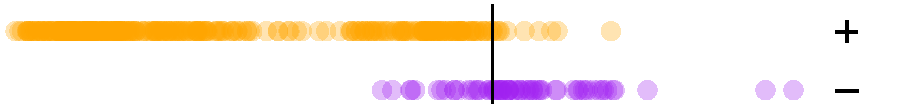
\includegraphics[width=0.4\textwidth]{chapter_spatial_voting_with_text/figures/3397_ideal_point_10.pdf}
 & 
\includegraphics[width=0.4\textwidth]{chapter_spatial_voting_with_text/figures/3397_adjusted_ideal_point_10.pdf} \\

%To restore sums to the Highway Trust Fund, and for other purposes
Providing for conditional adjournment/recess of Congress
%% NEWBORN Act \vspace{7pt}
%% Recess of the Houses \vspace{7pt}
%% Emergency Unemployment Compensation Continuation
%% Highway trust fund \vspace{7pt}
& 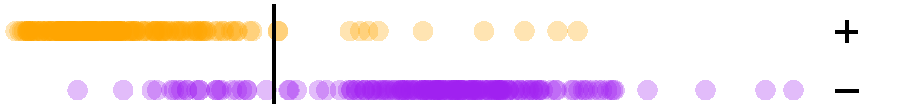
\includegraphics[width=0.4\textwidth]{chapter_spatial_voting_with_text/figures/3397_ideal_point_9.pdf}
& 
\includegraphics[width=0.4\textwidth]{chapter_spatial_voting_with_text/figures/3397_adjusted_ideal_point_9.pdf} \\

Establish R\&D program for gas turbines 
& 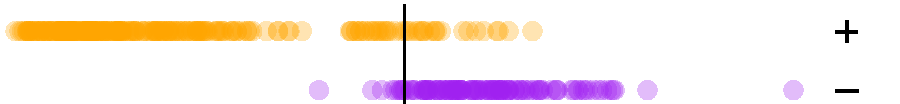
\includegraphics[width=0.4\textwidth]{chapter_spatial_voting_with_text/figures/3397_ideal_point_8.pdf}
& 
\includegraphics[width=0.4\textwidth]{chapter_spatial_voting_with_text/figures/3397_adjusted_ideal_point_8.pdf} \\

%Providing for an adjournment or recess of the two Houses
Recognizing AmeriCorps and community service
& 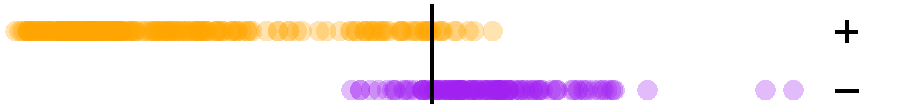
\includegraphics[width=0.4\textwidth]{chapter_spatial_voting_with_text/figures/3397_ideal_point_7.pdf}
& 
\includegraphics[width=0.4\textwidth]{chapter_spatial_voting_with_text/figures/3397_adjusted_ideal_point_7.pdf} \\

%Emergency Unemployment Compensation Continuation Act
Providing for conditional adjournment of Congress
& 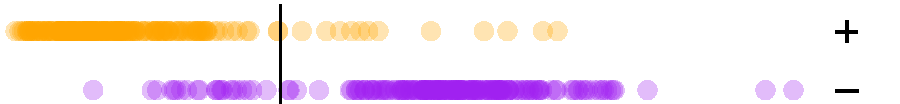
\includegraphics[width=0.4\textwidth]{chapter_spatial_voting_with_text/figures/3397_ideal_point_6.pdf}
& 
\includegraphics[width=0.4\textwidth]{chapter_spatial_voting_with_text/figures/3397_adjusted_ideal_point_6.pdf} \\

%Providing for a conditional adjournment of the House of Representatives & & \\
%and a conditional recess or adjournment of the Senate
Providing for the sine die adjournment of Congress
& 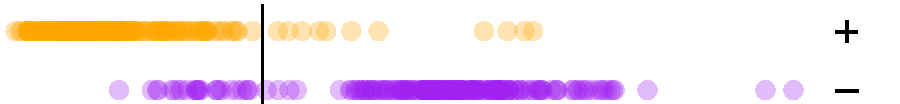
\includegraphics[width=0.4\textwidth]{chapter_spatial_voting_with_text/figures/3397_ideal_point_5.pdf}
& 
\includegraphics[width=0.4\textwidth]{chapter_spatial_voting_with_text/figures/3397_adjusted_ideal_point_5.pdf} \\

%Recognizing the significant accomplishments of AmeriCorps and
%encouraging... community service
Providing for an adjournment / recess of Congress
& 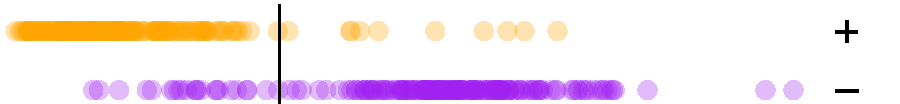
\includegraphics[width=0.4\textwidth]{chapter_spatial_voting_with_text/figures/3397_ideal_point_4.pdf}
& 
\includegraphics[width=0.4\textwidth]{chapter_spatial_voting_with_text/figures/3397_adjusted_ideal_point_4.pdf} \\

%Providing for the sine die adjournment of & & \\
%the first session of the One Hundred Eleventh Congress
Preventing child marriage in developing countries
& 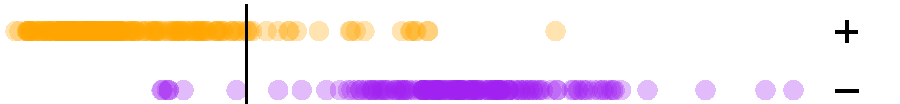
\includegraphics[width=0.4\textwidth]{chapter_spatial_voting_with_text/figures/3397_ideal_point_3.pdf}
& 
\includegraphics[width=0.4\textwidth]{chapter_spatial_voting_with_text/figures/3397_adjusted_ideal_point_3.pdf} \\

%A bill to protect girls in developing countries through the
%prevention of child marriage, and for other purposes
Providing for a conditional House adjournment
& 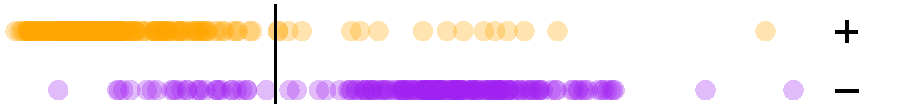
\includegraphics[width=0.4\textwidth]{chapter_spatial_voting_with_text/figures/3397_ideal_point_2.pdf}
& 
\includegraphics[width=0.4\textwidth]{chapter_spatial_voting_with_text/figures/3397_adjusted_ideal_point_2.pdf} \\

%Congratulating the 2009-2010 University of Maryland Men's
%Basketball Team, Greivis Vasquez, and Coach Gary Williams on an outstanding season
Congratulating UMD Men's basketball
& 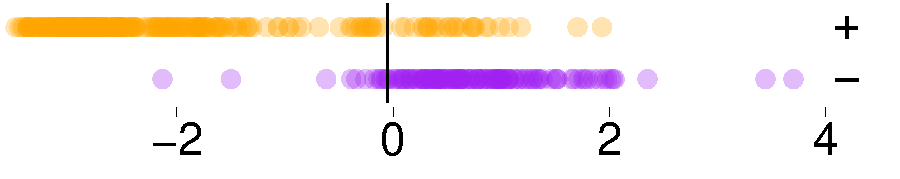
\includegraphics[width=0.4\textwidth]{chapter_spatial_voting_with_text/figures/3397_ideal_point_1.pdf}
& 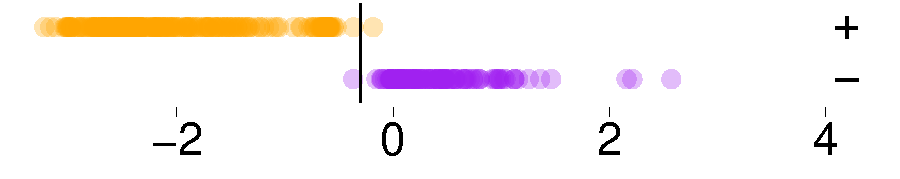
\includegraphics[width=0.4\textwidth]{chapter_spatial_voting_with_text/figures/3397_adjusted_ideal_point_1.pdf} \\
\hline
  \end{tabular}
%  \end{center}
\end{table}

\subsubsection{A comparison of issue-adjusted ideal points $x_u$ and traditional ideal points.}
The traditional ideal point model (\myeq{trad_ipm}) uses one parameter
per lawmaker---$x_u$---to explain all of her voting behavior.  In
contrast, the issue-adjusted model (\myeq{exploratory_ipm_old}) uses
$x_u$ along with seventy-four other parameters to describe each
lawmaker.  How does does $x_u$ under these two models differ?  We fit
ideal points to the 111th House (2009 to 2010) and issue-adjusted
ideal points $\tilde x_u$ to the same period ($\lambda=1$) and compare
these ideal points in \myfig{jackman_vs_offset}

In this figure we use an alternative to a scatterplot called a
\emph{parallel plot}.  In a parallel plot (which we will use several
more times in this article), we plot the two variables we wish to
compare along parallel axes and draw line segments connecting two
points when they represent the same variable under different
treatments.  In \myfig{jackman_vs_offset}, the top axis axis
represents a lawmaker's ideal point $x_u$ under traditional IRT, and
the bottom ``treatment'' axis represents his ideal point $x_u$ under
the issue-adjusted model.  Here and later we will use the convention
that the bottom row represents a special treatment. When it is
helpful, we use darker line segments for those items which change
the most under treatment.\footnote{Specifically, we fit a linear model
  to predict the bottom row from the top row and color line segments
  with opacity proportional to the squared residual of this pair. We
  specified opacity in \emph{ggplot} for \emph{R} with the alpha
  parameter.}

In the parallel plot in \myfig{jackman_vs_offset}, the traditional
ideal point model's $\tilde x_u$ and the issue-adjusted model's un-adjusted ideal
points $\tilde x_u$ are similar -- their correlation coefficient is
0.998. The most noteworthy change is that lawmakers appear more
partisan under the traditional ideal point model --- enough that
Democrats are completely separated from Republicans --- while
issue-adjusted ideal points provide a softer split.  This is not
surprising, because the issue-adjusted model is able to use lawmakers'
adjustments $\bm z_u$ to more than make up for this difference.  For
the same reason, issue-adjusted ideal points are slightly less extreme
than classic ideal points.

\begin{figure}
  \center
  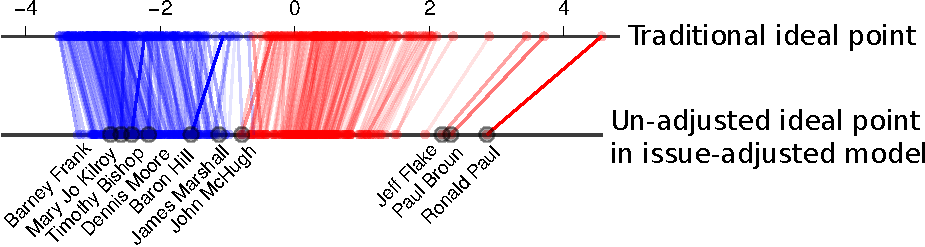
\includegraphics[width=0.8\textwidth]{chapter_spatial_voting_with_text/figures/3393_issue_vs_ideal_sxs.pdf}
  \label{figure:jackman_vs_offset}
  \caption{Classic issue-adjusted ideal points $x_u$ (top row) separate lawmakers by party better than un-adjusted ideal points $x_u$ from the
    issue-adjusted model (bottom row).  Republicans are colored red,
    and Democrats are blue.  These ideal points were estimated in
    the 111th House of Representatives.  The line connecting ideal points from
    each model has opacity proportional to the squared residuals in a linear
    model fit to predict issue-adjusted ideal points from ideal
    points. }
\end{figure}

%\subsection{Evaluation of the predictive distribution $p(v_{ud} | x_u, \bm z_u, a_u, b_u)$}
\subsubsection{Evaluation of the predictive distribution.}

The issue-adjusted model contains the ideal point model as the
special case $z_{uk}=0, \forall u, k$. Does this greater
expressivity---74 extra random variables per lawmaker---model
meaningful patterns?  We answer this question by comparing the
issue-adjusted ideal point model with two alternatives:

\begin{enumerate}
\item A variational ideal point model (\myeq{trad_ipm}), which treats
  lawmakers with the single variate $x_u$.

\item A permutation test.  The goal of this test is to attribute any
  improvement over traditional ideal points to the issues assigned to
  bills.  In this test, we randomly permute topic vectors' document
  labels: $(\bm \theta_1, \ldots, \bm \theta_D) \mapsto (\bm
  \theta_{\pi_i(1)} \ldots \bm \theta_{\pi_i(D)})$, for five random
  permutations $\pi_1, \ldots, \pi_{5}$.  This permutation test
  removes information contained in the matching from bills and topic
  mixtures.  At the same time, the empirical distribution over topic
  mixtures $\bm \theta_{dk}$ stays the same, and each bill is still
  matched to a topic mixture with $\sum_k \bm \theta_{dk} = 1$.  This
  is important because it any improvement we see over traditional
  ideal points is due to the bills' topics, not due to spurious
  factors (such as the change in dimension).
\end{enumerate}

\label{section:performance}
\paragraph{Sensitivity to $\lambda$.}
The main parameter in the issue-adjusted model is the regularization
$\lambda$, which is shared for all issue adjustments. We report the
effect of different $\lambda$ by fitting the issue-adjusted model to
the 109th Congress (1999-2000) of the House and Senate for a range
$\lambda=0.0001, \ldots, 1000$ of regularizations.  We performed
$6$-fold cross-validation, holding out one sixth of votes in each
fold, and calculated average log-likelihood $\sum_{v_{ud} \in
  V_{\mbox{\tiny heldout}}} \log p(v_{ud} | \tilde x_u, \bm \tilde
z_u, \tilde a_d, \tilde b_d)$ for votes $V_{\mbox{\tiny heldout}}$ in
the heldout set. Following the algorithm described in
\mysec{inference}, we began with $M=21$ samples to estimate the
approximate gradient (\myeq{taylor_approximation}) and scaled it by
1.2 each time the Elbo dropped below a threshold, until it was 500. We
also fixed variance $\sigma_x^2, \sigma_z^2, \sigma_a^2,
\sigma_b^2=\exp({-}5)$.  We summarize these results in
\mytab{lambda_comparison}.

The variational implementation generalized well for the entire range,
representing votes best in the range $1 \le \lambda \le 10$.
Log-likelihood dropped modestly for $\lambda < 1$.  In the worst case,
log-likelihood was -0.159 in the House (this corresponds with 96\%
heldout accuracy) and -0.242 in the Senate (93\% heldout accuracy).

\begin{table}
  \caption{Average log-likelihood of heldout votes by regularization
    $\lambda$. Log-likelihood was averaged across folds using six-fold
    cross validation for Congress 109 (2005-2006).  The variational
    distribution represented votes with higher heldout log-likelihood
    than traditional ideal points for $1 \le \lambda \le 10$. In a
    model fit with permuted issue labels (Perm. Issue), heldout
    likelihood of votes was worse than traditional ideal points for
    all regularizations $\lambda$.
  } \center \small
  \begin{tabular}{|c|cccccccc|}
    \hline
    \textbf{Model} & \multicolumn{8}{|c|}{\textbf{Senate}} \\
    \hline
    \textbf{$\lambda$}
    & 1e-4
    &  1e-3 
    &  1e-2 
    &  1e-1 
    &  1 
    &  10 
    &  100
    &  1000  \\
    \hline
    Ideal
    &  -0.188 % 1e-4
    &  -0.189 
    &  -0.189 % 1e-2
    &  -0.189
    &  -0.189 % 1
    &  -0.190 % 10
    &  -0.189
    &  -0.189  \\ % 1000
    Issue (LDA)
    & -0.191 % 1e-4
    & -0.191
    & -0.188 % 1e-2
    & -0.186 % 0.1
    & -0.188 % 1
    & -0.189
    & -0.189 % 100
    & 0.198 \\ 
     Perm. Issue 
    &  -0.242 
    &  -0.245 
    &  -0.231 
    &  -0.221 
    &  -0.204 
    &  -0.208 
    &  -0.208 
    &  -0.208  \\
    \hline
    \hline
    \textbf{Model} & \multicolumn{8}{|c|}{\textbf{House}} \\
    \hline
    \textbf{$\lambda$}
    & 1e-4
    &  1e-3 
    &  1e-2 
    &  1e-1 
    &  1 
    &  10 
    &  100
    &  1000  \\
    \hline
    Ideal
    &  -0.119 % 1e-4
    &  -0.119 
    &  -0.119 % 1e-2
    &  -0.119
    &  -0.120 % 1
    &  -0.119 % 10
    &  -0.119
    &  -0.119  \\ % 1000
    Issue (LDA)
    & -0.159 % 1e-4
    & -0.159
    & -0.158 % 1e-2
    & -0.139 % 0.1
    & -0.118 % 1
    & -0.119
    & -0.119 % 100
    & 0.119 \\ 
     Perm. Issue 
    &  -0.191 
    &  -0.192 
    &  -0.189 
    &  -0.161 
    &  -0.122 
    &  -0.120 
    &  -0.120 
    &  -0.120  \\
    \hline
  \end{tabular}
  \normalsize
  \label{table:lambda_comparison}
\end{table}

\paragraph{Performance across all sessions.}

\begin{table}
  \caption{Average log-likelihood of heldout votes across all sessions
    for the House and Senate.  Log-likelihood was averaged across
    folds using six-fold cross validation for Congresses 106 to 111
    (1999-2010) with regularization $\lambda=1$.  The variational
    distribution had higher heldout log-likelihood for all congresses
    in both chambers than either } \center \small
  \begin{tabular}{|c|cccccc|}
    \hline
    \textbf{Model} & \multicolumn{6}{|c|}{\textbf{Senate}} \\
    \hline
    \textbf{Congress} & \hspace{-4pt} 106 \hspace{-5pt}
    & \hspace{-4pt} 107 \hspace{-5pt}
    & \hspace{-4pt} 108 \hspace{-5pt}
    & \hspace{-4pt} 109 \hspace{-5pt}
    & \hspace{-4pt} 110 \hspace{-5pt}
    & \hspace{-4pt} 111 \hspace{-4pt} \\
    \hline
    Ideal
    & \hspace{-4pt} -0.209 \hspace{-5pt}
    & \hspace{-4pt} -0.209 \hspace{-5pt}
    & \hspace{-4pt} -0.182 \hspace{-5pt}
    & \hspace{-4pt} -0.189 \hspace{-5pt}
    & \hspace{-4pt} -0.206 \hspace{-5pt}
    & \hspace{-4pt} -0.182 \hspace{-4pt} \\
    Issue (LDA)
    & \hspace{-4pt} \textbf{-0.208} \hspace{-5pt}
    & \hspace{-4pt} \textbf{-0.209} \hspace{-5pt}
    & \hspace{-4pt} \textbf{-0.181} \hspace{-5pt}
    & \hspace{-4pt} \textbf{-0.188} \hspace{-5pt}
    & \hspace{-4pt} \textbf{-0.205} \hspace{-5pt}
    & \hspace{-4pt} \textbf{-0.180} \hspace{-4pt} \\
    Issue (label)
    & \hspace{-4pt} \textbf{-0.208} \hspace{-5pt}
    & \hspace{-4pt} \textbf{-0.209} \hspace{-5pt}
    & \hspace{-4pt} -0.182 \hspace{-5pt}
    & \hspace{-4pt} -0.189 \hspace{-5pt}
    & \hspace{-4pt} -0.206 \hspace{-5pt}
   & \hspace{-4pt} -0.181 \hspace{-4pt} \\
    \hspace{-5pt} Perm. Issue \hspace{-5pt}
    & \hspace{-4pt} -0.210 \hspace{-5pt}
    & \hspace{-4pt} -0.210 \hspace{-5pt}
    & \hspace{-4pt} -0.183 \hspace{-5pt}
    & \hspace{-4pt} -0.203 \hspace{-5pt}
    & \hspace{-4pt} -0.211 \hspace{-5pt}
    & \hspace{-4pt} -0.186 \hspace{-4pt} \\
    % Permuted Issue & & & & & & \\
    \hline
    \hline
    & \multicolumn{6}{|c|}{\textbf{House}} \\
    \hline
    Ideal & \hspace{-4pt} -0.168 \hspace{-5pt}
    & \hspace{-4pt} -0.154 \hspace{-5pt}
    & \hspace{-4pt} -0.096 \hspace{-5pt}
    & \hspace{-4pt} -0.120 \hspace{-5pt}
    & \hspace{-4pt} -0.090 \hspace{-5pt}
    & \hspace{-4pt} -0.077 \hspace{-4pt} \\
    Issue (LDA)
    & \hspace{-4pt} \textbf{-0.167} \hspace{-5pt}
    & \hspace{-4pt} \textbf{-0.151} \hspace{-5pt}
    & \hspace{-4pt} -0.095 \hspace{-5pt}
    & \hspace{-4pt} -0.118 \hspace{-5pt}
    & \hspace{-4pt} -0.089 \hspace{-5pt}
    & \hspace{-4pt} -0.076 \hspace{-4pt} \\
    Issue (label)
    & \hspace{-4pt} \textbf{-0.167} \hspace{-5pt}
    & \hspace{-4pt} \textbf{-0.151} \hspace{-5pt}
    & \hspace{-4pt} \textbf{-0.094} \hspace{-5pt}
    & \hspace{-4pt} \textbf{-0.117} \hspace{-5pt}
    & \hspace{-4pt} \textbf{-0.088} \hspace{-5pt}
    & \hspace{-4pt} \textbf{-0.075} \hspace{-4pt} \\
    \hspace{-5pt} Perm. Issue \hspace{-5pt}
    & \hspace{-4pt} -0.167 \hspace{-5pt}
    & \hspace{-4pt} -0.155 \hspace{-5pt}
    & \hspace{-4pt} -0.096 \hspace{-5pt}
    & \hspace{-4pt} -0.122 \hspace{-5pt}
    & \hspace{-4pt} -0.090 \hspace{-5pt}
    & \hspace{-4pt} -0.077 \hspace{-4pt} \\
    \hline
  \end{tabular}
  \normalsize
  \label{table:session_comparison}
\end{table}

We fit the issue-adjusted model to both the House and Senate for
Congresses 106 to 110 (1999-2010) with $\lambda=1$. For comparison we
also fit an ideal point model to each of these congresses and fit an
issue-adjusted model to each congress with topics' document labels
permuted ($\bm \theta_{\pi(1)}, \ldots, \bm \theta_{\pi(1)}$). We
summarize these results in Table~\ref{table:session_comparison}. In
all chambers in both Congresses, the issue-adjusted model represents
heldout votes with higher log-likelihood than an ideal point model.
Further, every permutation represented votes with lower log-likelihood
than the issue-adjusted model.  In most cases they were also lower
than an ideal point model.

% \subsection{Generalization}
% The variational implementation generalizes well for the entire range
% $\lambda = 0.0001, \ldots, 1000$, with classification accuracy peaking
% near $\lambda=1$.  Even in the worst case, accuracy remains above 96\%
% in the House.  This is striking, given the huge increase in parameter
% size for this model, and it contrasts sharply with the MAP estimate,
% which quickly overfit. With $\lambda < 10$, MAP training accuracy
% approached 100\% while its test accuracy quickly dropped. For
% $\lambda=10$, MAP issue adjustments $Z_{uk}$ were sometimes greater
% than $15$.  We believe the difference between these posterior
% estimates can be explained by the MAP implementation reaching poor
% local optima.

\paragraph{Human labels vs. inferred text-based labels.}
The issue-adjusted model assumes a fixed issue vector $\bm \theta_d$
for each bill.  We described a method in \mysec{lda} for inferring
this issue vector based on the text of bills using labeled LDA; this
method uses the original Congressional Research Service (CRS) labels.
What happens if we skip this preprocessing step and just use the
original CRS labels? We checked this by converting the original CRS
issue labels into a $K$-vector of issues.  For each document $d$
having issue labels $J \subset K$, each issue $\bm \theta_{dk}$ was
assigned a weight of $1 / |J|$ if $k \in J$ and zero if $k \not \in
J$. We fit an issue-adjusted model using these with CRS labels and
performed six-fold cross validation as described above and illustrate
predictive performance in \mytab{session_comparison} in the ``Issue
(label)'' row.

Across Congresses, the predictive benefit in using text-based issue
vectors over labels provided by the CRS is negligible.  However, we
see at least two benefits in using text-based labels.  First, they
provide a defensible way to distribute weight to each issue: an issue
should receive less than $1 / |J|$ weight if it is mentioned only in
passing in a bill.  Second, this method allows us to fit issue vectors
to the 107 bills which were missing CRS labels.

\paragraph{Changes in bills' parameters.}
Bills' polarity $a_d$ and popularity $b_d$ are similar under both the
traditional ideal point model and the issue-adjusted model. We
illustrate bills' parameters in these two models in
\myfig{bills_parameter_changes} and note two exceptions.  First,
procedural bills stand out from other bills in becoming more popular
overall.  In \myfig{bills_parameter_changes}, procedural bills have
been separated from traditional ideal points.  We attribute the
difference in procedural bills' parameters to \emph{procedural cartel
  theory}, which we describe further in
\mysec{procural_cartel_theory}.  Second, the remaining bills have
become less popular but more polarized under the issue-adjusted model.
This is because the model depends more on lawmakers' positions to
explain votes, because it has many more dimensions with which it can
describe each lawmaker.
\begin{figure}
  \begin{tabular}{|m{0.85in}|m{2.54in}|m{2.54in}|}
%    \Large \textbf{Polarity $a_d$} & \Large \textbf{Popularity $b_d$} \\
    \hline
    & Popularity & Polarity \\
    \hline
    Not procedural &
    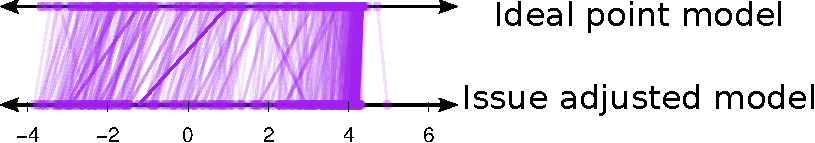
\includegraphics[width=0.4\textwidth]{chapter_spatial_voting_with_text/figures/3398_noprocedural_popularity.pdf} &
    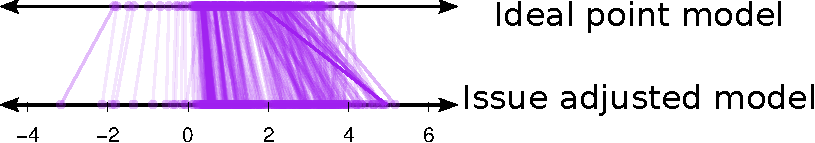
\includegraphics[width=0.4\textwidth]{chapter_spatial_voting_with_text/figures/3398_noprocedural_polarity.pdf} \\
    Procedural &
    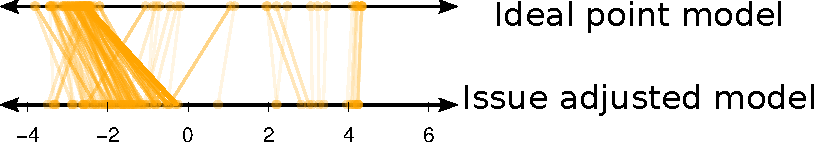
\includegraphics[width=0.4\textwidth]{chapter_spatial_voting_with_text/figures/3398_procedural_popularity.pdf} &
    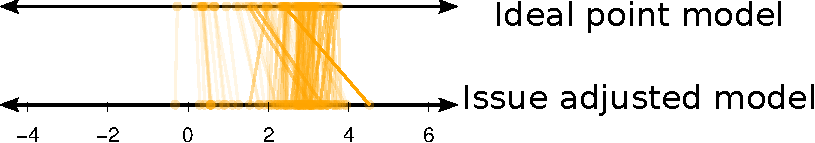
\includegraphics[width=0.4\textwidth]{chapter_spatial_voting_with_text/figures/3398_procedural_polarity.pdf} \\
    \hline
  \end{tabular}
  \caption{Procedural bills are more popular under the issue-adjusted
    voting model. Top: popularity $b_d$ of procedural bills under the
    issue-adjusted voting model is greater than with traditional ideal
    points.  Bottom: consistent with \citet{cox:2002} and
    \emph{procedural cartel theory}, the polarity of procedural bills
    is generally more extreme than that of non-procedural bills.
    However, issue adjustments lead to increased polarity (i.e.,
    certainty) among non-procedural votes as well.  The procedural
    issues include \emph{Congressional reporting requirements},
    \emph{Government operations and politics}, \emph{House of
      Representatives}, \emph{House rules and procedure},
    \emph{Legislative rules and procedure}, and \emph{Congress}.}
  \label{figure:bills_parameter_changes}
\end{figure}

\paragraph{Sparsity of $\tilde z_{uk}$.}
The variational estimates $\tilde z_{uk}$ of issue adjustments were
not sparse, although a high mass of thse issue adjustments was
concentrated around zero: twenty-nine percent of issue adjustments
were within $[-0.01, 0.01]$, and eighty-seven percent of issue
adjustments were within $[-0.1, 0.1]$.  We illustrate the distribution
of lawmakers' offsets for selected issues in
\myfig{issue_adjustment_distribution} and describe them further in
\mysec{lawmakers}.

% \section{Bills}

% Issue-adjusted ideal points are not not used in a vacuum, of course:
% the very fact that a bill is about an issue provides us with
% information on how lawmakers feel about the issue.  The goal of the
% next three sections is to provide a closer perspective on the way
% issues improve the way we represent votes on bills, lawmakers, and
% specific issues.

\subsection{Issues and Lawmakers}

\label{section:lawmakers}
\label{section:issues}

We illustrate Representatives' issue adjustments for the issues
\emph{Finance} and the procedural issue \emph{Congressional sessions}
in \myfig{issue_improvements_ideals} for the 111th House.  These
adjustments illustrate the way in which the issue-adjusted voting
model allows us to better understand how lawmakers feel about specific
issues, but they do not tell us which issues were well-fit by the
model, or whether these issue adjustments were systemic (i.e.,
predictable using lawmakers' ideal points) or even statistically
significant.

The goal of this section is to address these concerns by providing a
qualitative look at lawmakers' issue preferences such as those in
\myfig{issue_improvements_ideals}.  We begin by identifying those
issues which were best- and worst-represented by the issue-adjusted
model.  We then look at when lawmakers' issue adjustments can be
explained by party affiliation and discuss how to control for these
systemic biases to identify lawmakers who trascend party lines.  We
finally describe a theory explaining why certain lawmakers have such
different preferences on procedural issues like \emph{Congressional
  sessions} than substantive issues like as \emph{Finance}.

\subsubsection{Issues improved by issue adjustment.}
Those issues which tended to move lawmakers the most (by standard
deviation of $\hat z_k$) also tended to give issue-adjusted ideal
points an edge over traditional ideal points.  We measure the
performance improvement for any issue by first taking the
issue-adjusted log likelihood of each vote
\begin{equation}
  J_{ud} = 1_{\{v_{ud} = \mbox{yes}\}} p - \log(1 + \exp(p)),
\end{equation}
where $p = (x_u + \bm z_{u}^T \bm \theta_d ) a_d + b_d$ is the
log-odds of a vote under the issue adjusted voting model.  We also
measure the corresponding log-likelihood $I_{ud}$ under the ideal
point model, using $p=x_u a_d + b_d$ with an ideal point model. The
improvement of issue $k$ is then the sum of the improvement in
log-likelihood, weighted by issue $k$:
\begin{equation}
  \label{equation:likelihood_improvement}
  \mbox{Imp}_k = \frac{\sum_{v_{ud}} \bm \theta_{d_v k} (J_{ud} - I_{ud}) }
       { \sum_{v_{ud}} \bm \theta_{d_v k} }.
\end{equation}
A high value of $\mbox{Imp}_k$ indicates that issue $k$ is associated
with an increase in log-likelihood, while a low value is associated
with a decrease in log-likelihood.

\begin{figure}
  \center
  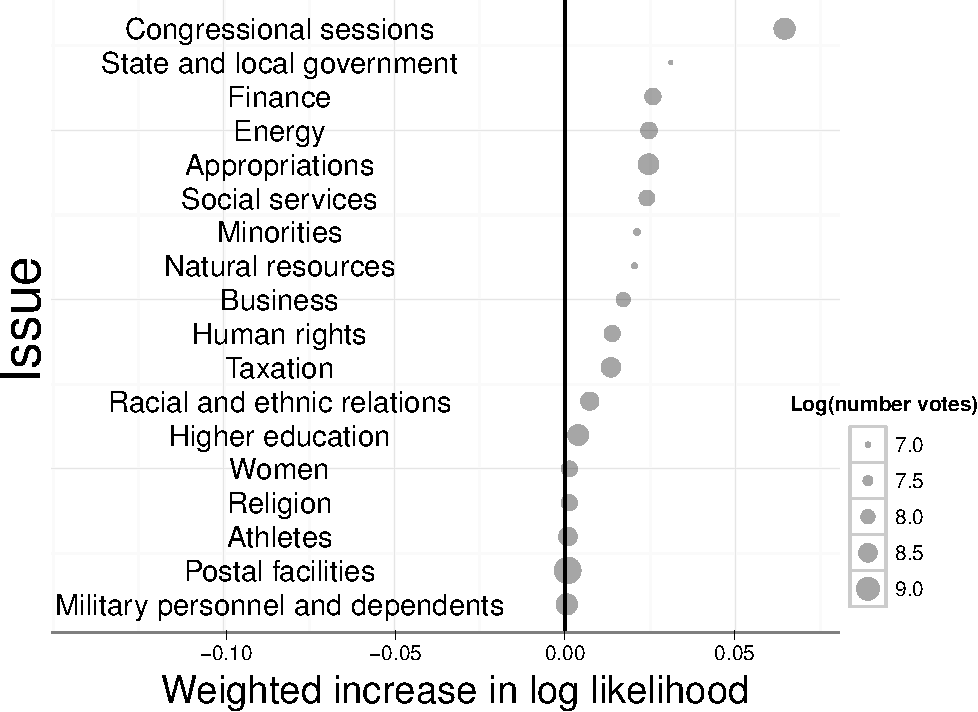
\includegraphics[width=0.6\textwidth]{chapter_spatial_voting_with_text/figures/3393_interesting_offsets.pdf}
  \caption{Log-likelihood increases when using adjusted ideal points
  most for procedural and strategic votes and less for issues
  frequently discussed during elections.  $\mbox{Imp}_k$ is shown on
  the x-axis, while issues are spread on the y-axis for display.
  The size of each issue $k$ is proportional to the logarithm of the
  weighted sum $\sum_{v_{ud}} \bm \theta_{dk}$ of votes about the
  issue.}
  \label{figure:issue_improvements}
\end{figure}
We illustrate $\mbox{Imp}_k$ for a selection of issues in
Figure~\ref{figure:issue_improvements}.  All issues increased
log-likelihood; those associated with the greatest increase tended to
be related to procedural votes.  For example, \emph{Women},
\emph{Religion}, and \emph{Military personnel} issues are nearly
unaffected by lawmakers' offsets.  These improvements $\mbox{Imp}_k$
were correlated with the standard deviation of residual offsets $\hat
z_k$ ($\sigma_{\mbox{cor}}=0.68$), but not with coefficients $\beta_k$
($\sigma_{\mbox{cor}}=0.05$), indicating that issue offsets, and not
ideal points, explain most of the improvement.

\paragraph{Issues associated with worse predictions.}
We also note several poorly-fit issues.  We evaluated issues by taking
the number of incorrectly-fit votes under the issue-adjusted model
\emph{minus} the number of incorrectly-fit votes under a traditional ideal
point model.  We call this the number of ``new mis-predicted votes''
for each issue.  Those issues which had the most ``new mis-predicted
votes'' also had the most ``new correctly-predicted votes'', which is
largely because votes on these issues are simply hard to predict.  For
example, \emph{Athletics} was one of the issues which saw the most
most newly-mispredicted votes.  \emph{Postal Facilities} and
\emph{Military Personnel} were other examples.

Bills which expressed many issues were also less-well fit.  The bill
which decreased the most by log-likelihood of its votes from the ideal
point model in the 111th House was the \emph{Consolidated Land,
  Energy, and Aquatic Resources Act of 2010} (H.R. 3534).  This bill
had substantial weight in five issues, with most in \emph{Public lands
  and natural resources}, \emph{Energy}, and \emph{Land transfers},
but its placement in many issues appears to have harmed its
performance.  This effect was common, and it suggests that methods
which represent bills with fewer issues (such as unsupervised topics)
may perform better, at the expense of interpretability.

\subsubsection{Understanding legislators' voting amidst party bias.}
\label{section:party_bias}
Many lawmakers' issue adjustments can be explained by party
affiliation (hence, their ideal point).  We illustrate the
distribution across lawmakers of $\tilde z_{uk}$ for selected issues
$k$ in \myfig{issue_adjustment_distribution}.  This figure shows this
distribution for the four issues with the greatest variance in $\tilde
z_{uk}$ across lawmakers and the four issues with the least variance
across lawmakers. Note the systematic bias in Democrats' and
Republicans' issue preferences: they become \emph{more partisan} on
certain issues, particularly procedural ones.

\begin{figure}
  \center
  \begin{tabular}{cc}
    \Large \textbf{Democrat} & \Large \textbf{Republican} \normalsize \\
  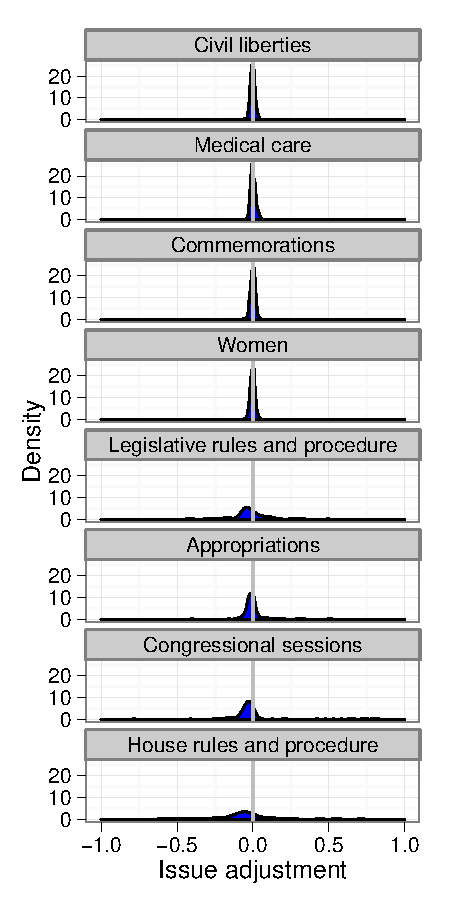
\includegraphics[width=0.45\textwidth]{chapter_spatial_voting_with_text/figures/3393_issue_adjustment_density_democrats.pdf} &
  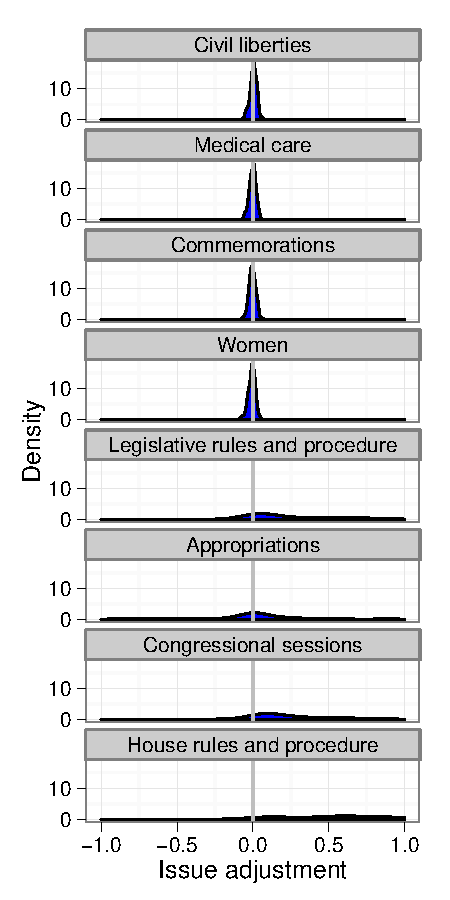
\includegraphics[width=0.45\textwidth]{chapter_spatial_voting_with_text/figures/3393_issue_adjustment_density_republicans.pdf} \\
  \end{tabular}
  \caption{Histogram of issue adjustments for selected
    issues. Democrats are in the left column, and Republicans are in
    the right column. Both Democrats and Republicans tend to have
    small issue adjustments for traditional issues.  Their issue
    adjustments differ substantially for procedural issues. A
    more-dispersed distribution of issue adjustments does not mean
    that these lawmakers tend to feel differently from one another
    about these issues.  Instead, it means that lawmakers deviate from
    their ideal points more.  }
  \label{figure:issue_adjustment_distribution}
\end{figure}

%\subsection{Checking issue affinity}
\label{section:conditional_offets}

\paragraph{Controlling for ideal points.}

A typical Republican tends to have a Republican offset on taxation,
but this surprises nobody.  Instead, we are more interested in
understanding when this Republican lawmaker \emph{deviates} from
behavior suggested by her ideal point.  We can shed light on this
systemic issue bias by explicitly controlling for it.  To do this, we
fit a regression for each issue $k$ to explain away the effect of a
lawmaker's ideal point $\bm x_u$ on her offset $\bm z_{uk}$:
\[
  \bm z_{k} = \beta_k \bm X + \bm \varepsilon,
\]
where $\beta_k \in \mathbb{R}$.  Instead of evaluating a lawmaker's
observed offsets, we use her residual $\hat z_{uk} = \bm z_{uk} -
\beta_k \bm x_u$, which we call the corrected issue adjustment.  By
doing this, we can evaluate lawmakers in the context of other
lawmakers who share the same ideal points: a positive offset $\hat
z_{uk}$ for a Democrat means she tends to vote more liberally about
issue $k$ than others with the same ideal point (most of whom are
Democrats).\footnote{We also fit a model with this regression
  explicitly encoded.  That model performed slightly worse in
  experiments on heldout data.}

% \paragraph{Distribution of issue adjustments}
Most issues had only a moderate relationship to ideal points.
\emph{House rules and procedure} was the most-correlated with ideal
points, moving the adjusted ideal point $\beta_k=0.26$ right for every
unit increase in ideal point. \emph{Public land and natural resources} and
\emph{Taxation} followed at a distance, moving an ideal point $0.04$
and $0.025$ respectively with each unit increase in ideal point.
\emph{Health}, on the other hand, moved lawmakers $\beta_k=0.04$ left
for every unit increase in ideal point.
\begin{figure*}[t]
  \center
  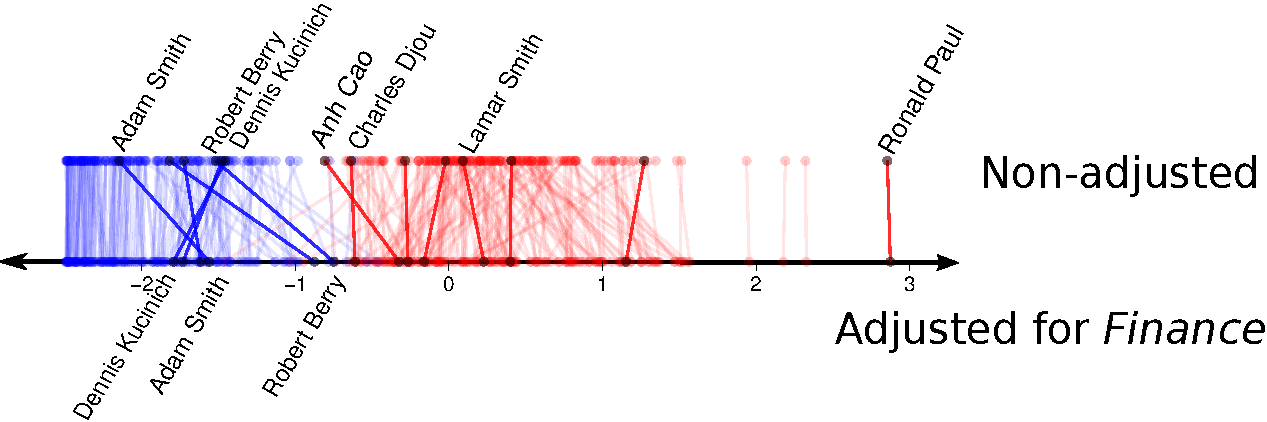
\includegraphics[width=0.77\textwidth]{chapter_spatial_voting_with_text/figures/3393_example_ideal_points_finance.pdf}
  \vspace{-10pt}
  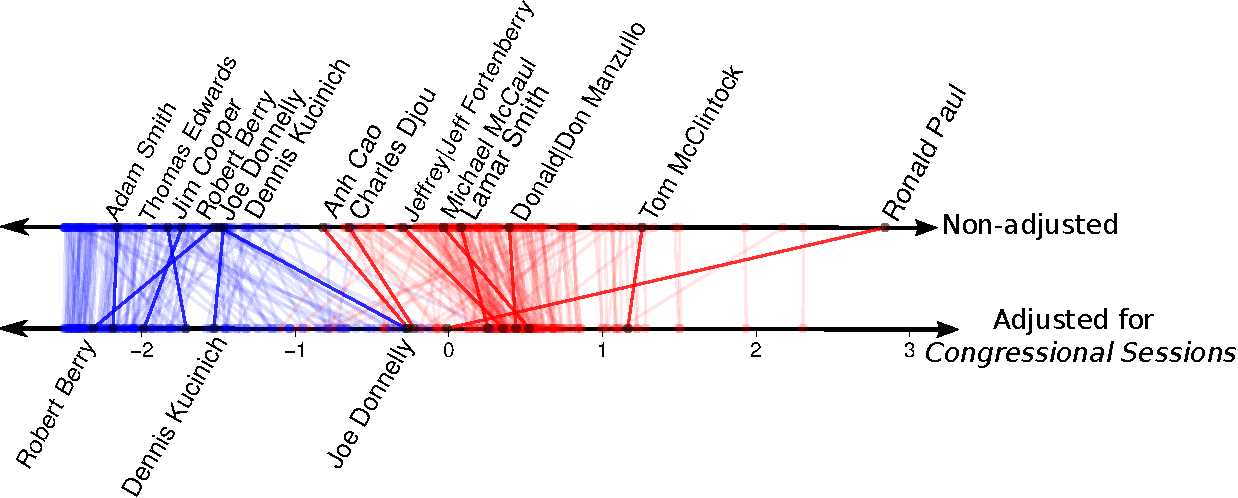
\includegraphics[width=0.85\textwidth]{chapter_spatial_voting_with_text/figures/3393_example_ideal_points_congressional_sessions.pdf}
  \caption{Ideal points $x_u$ and issue-adjusted ideal points $x_u +
    z_{uk}$ from the 111th House for the substantive issue
    \emph{Finance} and the procedural issue \emph{Congressional
      Sessions}. Democrats are blue and Republicans are red.  Votes
    about \emph{Finance} and \emph{Congressional Sessions} were better
    fit using issue-adjusted ideal points.  For procedural votes such
    as \emph{Congressional sessions}, lawmakers becoming more
    polarized by political party, behavior predicted by procedural
    cartel theory \citep{cox:1993}. }
  \label{figure:issue_improvements_ideals}
  \vspace{-5pt}
\end{figure*}
The issues \emph{Women}, \emph{Religion}, and \emph{Military
personnel} were nearly unaffected by lawmakers' offsets.
%% We will take a closer look at this metric when we discuss specific
%% lawmakers in the next section.

\paragraph{Finding exceptional issue-adjustments.}

%% The issue-adjusted ideal point model usually fit votes better than the
%% ideal point model, but there were some exceptions.  In the 111th
%% House, lawmakers were almost invariably improved with issue-adjusted
%% ideal points.  Only Representative Steve Kagan (Democrat from Ohio),
%% had lower training log likelihood with the issue-adjusted model than
%% with an ideal point model.  This decrease was negligible, and Kagan's
%% votes were very-well represented with both traditional and adjusted
%% ideal points.

% \section{Issues}
%% A handful of lawmakers stood out with the most exceptional issue
%% adjustments.  Any reference in this section to lawmakers' issue
%% adjustments refers to lawmakers' residuals $\hat z_{uk}$ fit from
%% their variational parameters $\bm \tilde z_{uk}$.

We next use these corrected issue adjustments to identify lawmakers'
exceptional issue preferences. To identify adjustments which are
significant, we turn again to the same nonparametric check described
in the last section: permute issue vectors' document labels,
i.e. $(\bm \theta_1, \ldots, \bm \theta_D) \mapsto (\bm \theta_{\pi_i(1)} \ldots \bm \theta_{\pi_i(D)})$, and refit lawmakers'
adjustments using both the original issue vectors and permuted issue
vectors, for permutations $\pi_1, \ldots, \pi_{20}$.  We then compare
a corrected issue adjustment $\hat z_{uk}$'s absolute value with
corrected issue adjustments estimated with permuted issue vectors $\bm
\theta_{\pi_i(d) k}$.

This provides a nonparametric method for finding issue adjustments
which are more extreme than expected by chance: an extreme issue
adjustment has a greater absolute value than all of its permuted
counterparts.  We use these to discuss several unique lawmakers.
% (those with four or more significant offsets (p < 0.006).
%% # 0 significant: 0.471
%% # 1 significant: 0.357
%% # 2 significant: 0.133  // cdf: 0.961
%% # 3 significant: 0.033  // cdf:  0.994 one in two hundred.

\begin{figure*}
  %  \includegraphics[width=0.5\textwidth]{chapter_spatial_voting_with_text/figures/3293_Russell_Feingold_300042.pdf}
  %  \includegraphics[width=0.5\textwidth]{chapter_spatial_voting_with_text/figures/3293_Evan_Bayh_300006.pdf} \\
%    \includegraphics[width=0.5\textwidth]{chapter_spatial_voting_with_text/figures/3293_Thomas_Tom_Carper_300019.pdf} &
    %Ken Salazar & Robert Casey \\
    %\includegraphics[width=0.5\textwidth]{chapter_spatial_voting_with_text/figures/3293_Ken_Salazar_400619.pdf} &
%    \includegraphics[width=0.5\textwidth]{chapter_spatial_voting_with_text/figures/3293_house_Dennis_Kucinich_400227.pdf} \\
%    \includegraphics[width=0.5\textwidth]{chapter_spatial_voting_with_text/figures/3293_house_James_McDermott_400262.pdf} \\
  \center
  \begin{tabular}{cc}
%     Bob Casey
    %\includegraphics[width=0.3\textwidth]{chapter_spatial_voting_with_text/figures/3293_Robert_Casey_412246.pdf} &
%    \includegraphics[width=0.24\textwidth]{chapter_spatial_voting_with_text/figures/3393_Russell_Feingold_300042.pdf} &
%    \includegraphics[width=0.24\textwidth]{chapter_spatial_voting_with_text/figures/3393_George_Voinovich_300098.pdf} &
%    Ronald Paul & Mark Critz \\
    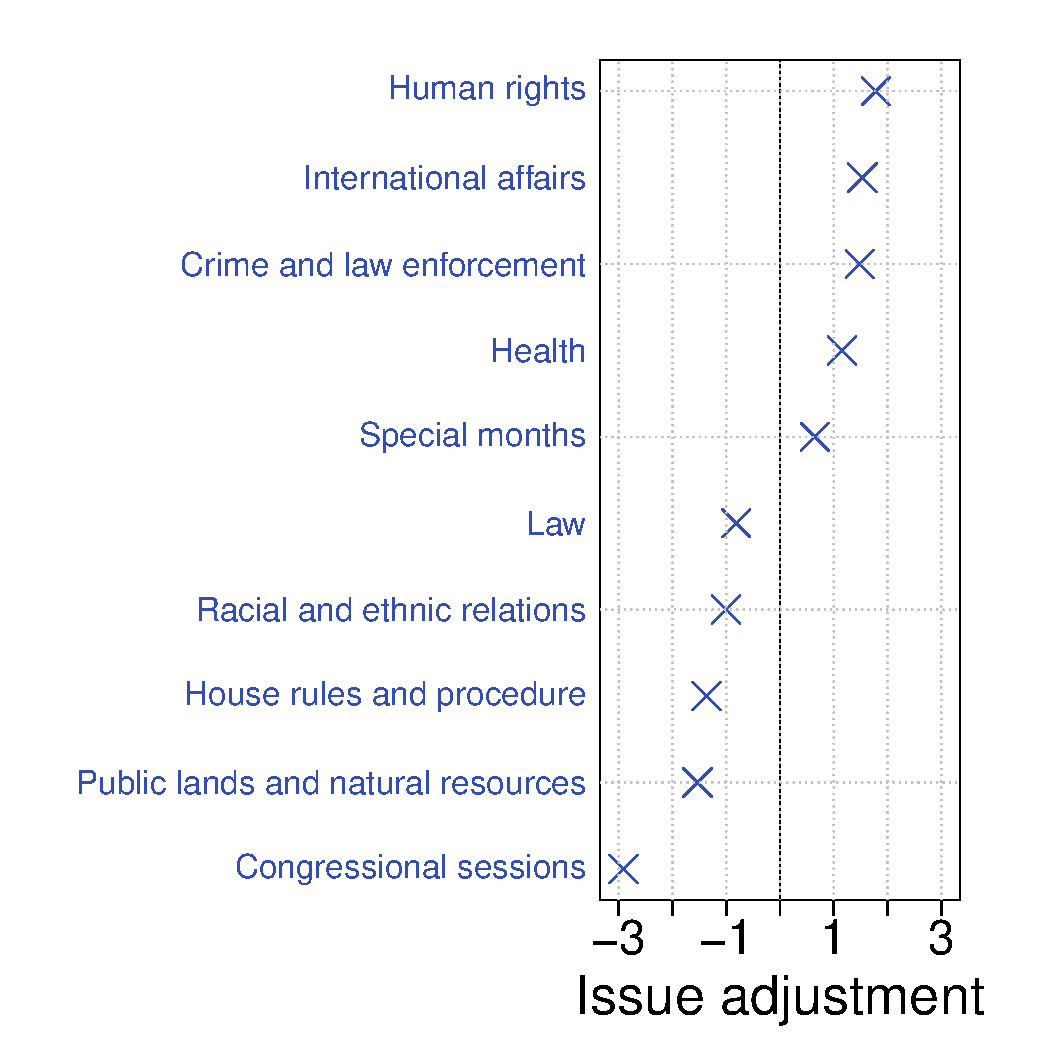
\includegraphics[width=0.5\textwidth]{chapter_spatial_voting_with_text/figures/3393_house_Ronald_Paul_400311.pdf} &
    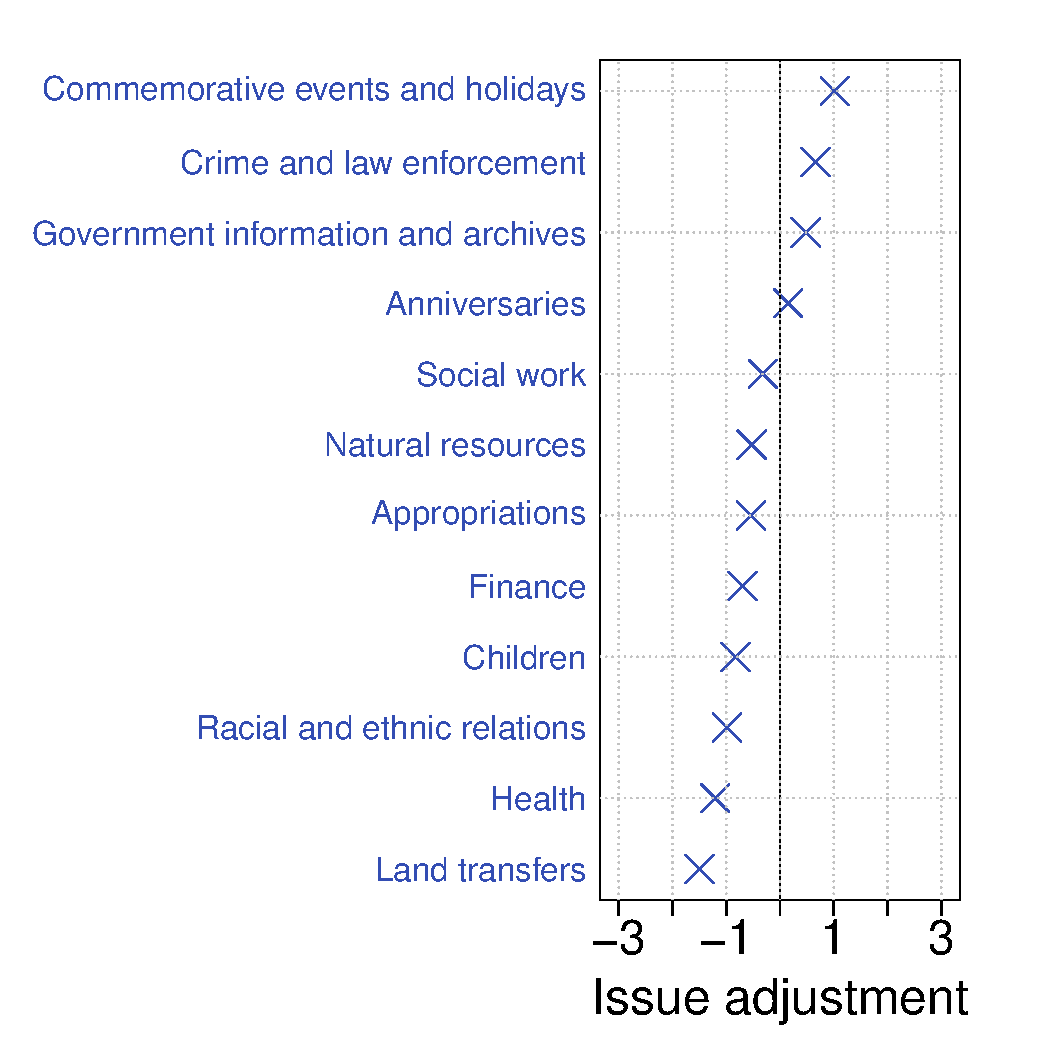
\includegraphics[width=0.5\textwidth]{chapter_spatial_voting_with_text/figures/3393_house_Donald_Young_400440.pdf} \\
    Ronald Paul (House Republican) & Donald Young (House Republican) \\
%    \includegraphics[width=0.24\textwidth]{chapter_spatial_voting_with_text/figures/3393_house_Mark_Critz_412386.pdf} \\
%    \includegraphics[width=0.24\textwidth]{chapter_spatial_voting_with_text/figures/3393_house_Baron_Hill_400177.pdf} \\
%    Russell Feingold (Senate Democrat) & George Voinovich (Senate Republican) & Ronald Paul (House Republican) & Baron Hill (House Democrat) \\
%    Russell Feingold (Senate Democrat) & George Voinovich (Senate Republican) & Ronald Paul (House Republican) & Mark Critz (House Democrat) \\
  \end{tabular}
    \caption{Significant issue adjustments for exceptional senators in
  Congress 111.  Each illustrated issue is significant to $p <
  0.05$ by a permutation test.}
  \label{figure:significant_offsets}
\end{figure*}

%% \subsubsection{Posterior Predictive Checks}

%% Posterior predictive checks provide a way to check certain assumptions
%% made by a statistical model \citep{gelman:1996}. A posterior predictive
%% check compares the observed data set of votes $V^{\mbox{obs}}$ (earlier
%% we called this $V$) with replicated draws $V^{\mbox{rep}}$ from the
%% posterior:
%% \begin{equation}
%%   V^{\mbox{rep}}_1, \ldots, V^{\mbox{rep}}_N \sim p(V | V^{\mbox{obs}})
%%   \label{equation:sampled_votes}
%% \end{equation}
%% These samples are compared by defining a real-valued function $T$
%% (called a \mbox{discrepancy}) of a data set, sampled or not, and using
%% standard $p$-values to determine whether the observed data set is
%% significantly different than the replicated data sets.

%% The choice of discrepancy $T$ is important because it determines what
%% conclusions we can draw about the model.  It therefore must be
%% selected to inform model criticism. Note that these checks are
%% flexible: we can incorporate external constants into it, and we can
%% apply any check to individual lawmakers.

%% We first describe a check which can help to diagnose posterior
%% over-fitting.  For this check, we sample 250 sets of votes from the
%% \emph{variational} posterior $q_{\bm \eta}(X, \bm Y, \bm Z, A, B)$ as
%% in Equation~\ref{equation:sampled_votes}. For a discrepancy function,
%% we define the discrepancy $T$ to be the average log-likelihood of the
%% set of votes \emph{given the variational point-estimate}: $T(V) :=
%% \expectp{ \log p(V | X = \tilde X, \ldots, B = \tilde B)}$.  Ideally,
%% $T(V)$ will be high for both observed and sampled votes, and
%% $T(V^{\mbox{obs}})$ will not be significantly different from
%% $T(V^{\mbox{obs}})$.

%% \begin{figure}
%%   \center
%%   \includegraphics[height=0.4\textheight]{chapter_spatial_voting_with_text/figures/3250_training_ppc.pdf} \\
%%   \includegraphics[height=0.4\textheight]{chapter_spatial_voting_with_text/figures/3250_test_ppc.pdf} \\
%%   \caption{The likelihood of votes sampled from the variational
%%   posterior $q(x)$ (blue lines) against the likelihood of observed
%%   votes (black lines).  On top is training samples, while on bottom
%%   are test samples.}
%%   \label{figure:ppc_lawmakers}
%% \end{figure}

%% Figure~\ref{figure:ppc_lawmakers} (top) shows this discrepancy for a
%% selection of lawmakers discussed in
%% Section~\ref{section:exceptional_lawmakers}. Here we compare votes
%% sampled from the variational posterior with votes observed in a
%% $\frac{5}{6}$ training fold of the $111$th House.\footnote{For
%% reference, a log-likelihood of -0.5 is about the same as guessing 80\%
%% of votes correctly, and a log-likelihood of -0.3 is the same as
%% predicting 91\% of votes correctly.} In both cases, the discrepancy
%% above was used.  In most cases, the likelihood of the observed votes is
%% significantly higher than the likelihood of sampled votes.

%% This is not surprising, because we are using the data twice: first to
%% fit the posterior, and second to define the discrepancy.  The
%% variational point estimate is, further, defined to be the mode of the
%% distribution.  We therefore repeat this exercise for votes in a
%% held out fold, shown in Figure~\ref{figure:ppc_lawmakers}
%% (bottom).  In the latter case, the log-likelihood of samples is
%% evaluated using held out votes.  The spread of sampled likelihoods is
%% larger in the test set than in the training set because these pairs
%% were unobserved during training. At the same time, a significant
%% number of lawmakers stand out as being very-well predicted and being
%% very-poorly predicted.

%% \paragraph{Misplaced confidence in votes.}
%% The model tends to over-predict the likelihood of votes by lawmakers
%% like Donald Young and Ron Paul: for both, the simulated votes had
%% higher likelihood than held out votes.  This can be explained by either
%% bias in the estimates or under-predicting variance.  In a scatter plot
%% plot of lawmakers' variance, neither lawmaker stood out as
%% exceptional.

%% At the opposite extreme, the model tends to under-predict the
%% log-likelihood of lawmakers such as Duncan Hunter and John Murtha.
%% This can be explained by high variance in the prediction: the model
%% places highest probability on the observed votes and lower probability
%% on a typical, sampled vote.  In a scatter plot, both lawmakers had
%% moderately high variance.

%% Note that we cannot draw these conclusions from this check on the
%% training folds alone: we would nearly always infer that the model
%% should have lower variance if that were the case.

%\subsection{Voting by issue affinity}

%% \label{section:exceptional_lawmakers}
%% One of the more interesting questions we can inspect is, ``which
%% lawmakers make exceptional votes, and how are these votes
%% exceptional?'' The parameters $\bm Z_u$ provide an indication of this:
%% they capture lawmakers' exceptional voting patterns.

%% We consider this question in a fit of the House of Representatives in
%% the 111th Congress. This period was the first term of Barack Obama's
%% presidency, a period during which Democrats held a majority in both
%% the Senate (by a modest margin) and the House (by a large margin).
%% With gasoline and health care prices soaring and the Great Recession
%% taking hold as housing markets collapsed, significant legislation
%% passed or considered during this time included the Patient Protection
%% and Affordable Care Act (i.e., the ``Health Care Bill'') and
%% legislation aimed at regulating Wall Street.  We used MAP estimates
%% because they were accessible at the time this section was written.

%% \subsubsection{Identifying exceptional issue voting}

%% We can create a one-dimensional description of each lawmaker's
%% uniqueness by using their sum-of-squared offsets $\bm \tilde Z_u^T \bm
%% \tilde Z_u$. Lawmakers whose votes are typical will have relatively
%% small residual sum-of-squares, while those whose votes stand out will
%% have a much larger squared residual.

%% We considered these offsets in a fit of a labeled topic model with 74
%% labeled topics (see Section~\ref{section:lda} for a description of how
%% these topics were obtained). Selected lawmakers' \emph{effective ideal
%% points} $X_u + (X_u \bm Y + \bm Z_u)^T \bm \theta_d$ on a sample of
%% topics are provided in
%% Figure~\ref{figure:lawmaker_subset_ideal_points}.
%% %Figure~\ref{figure:lawmaker_ideal_points} shows a random sample of
%% %lawmakers (most of whom have a fairly low offset).

%% \begin{figure*}
%%   \center
%%   \includegraphics[width=0.9\textwidth]{chapter_spatial_voting_with_text/figures/3240_example_lawmaker_ips.pdf}
%%   \caption{Sum-of-squared lawmaker offset $\bm \tilde z^T \bm \tilde z$ vs. Ideal Point.  Selected lawmakers are labeled.}
%%   \label{figure:sso_by_ip}
%% \end{figure*}

%% \begin{figure*}
%%   \includegraphics[width=1.0\textwidth]{chapter_spatial_voting_with_text/figures/3240_legislator_subset_topics.pdf}
%%   \caption{Legislator topic intercepts for selected lawmakers and
%%     topics.  Ideal point offsets $[0, X_u]$ are grey; the interval $[
%%     X_u, X_u + X_u y_k ]$ is light and colored, and the interval $[X_u
%%     + X_u y_k, X_u + X_u y_k + Z_{uk}]$ (which is each lawmaker's
%%     distinctive style) is given by a dark bar.  A lawmaker's
%%     \emph{effective ideal point} $X_u + X_u y_k + Z_{uk}$ for each
%%     topic is given by the crosshairs.  This figure used 74 labeled
%%     topics and $\lambda=10$.}
%%   \label{figure:lawmaker_subset_ideal_points}
%% \end{figure*}
\paragraph{Extreme lawmakers.}

Using corrected issue adjustments, we identified several of the
most-unique lawmakers.  We focused this analysis on votes from
2009-2010, the most recent full session of Congress, using
$\lambda=1$.  We fit the variational model to all votes in the House
and computed lawmakers' corrected issue adjustments $\hat z_{uk}$, which are
conditioned on their ideal points as described in
Section~\ref{section:conditional_offets}.
Figure~\ref{figure:significant_offsets} illustrates those issue
preferences for several lawmakers from this Congress which significant
under 20 permutation replications ($p < 0.05$).

%\paragraph{Thomas Carper.} Senator Tom Carper, Democrat from 
%\paragraph{Judd Gregg.} Judd Gregg, former Republican Senator of New Hampshire, was one of the most unique Senators of the 111th Congress.  Gregg is known for holding positions.  The issue-adjusted model found that Gregg leans conservatively regarding Race and Ethnicities, 

%% \paragraph{Robert Casey.} Senator Casey, a Democrat from Pennsylvania,
%% was one of the most unique Democratic Senators, having voted with his
%% party 93\% of the time.  As a member of the Senate Committee on
%% Health, Education, Labor and Pensions, Casey held strong positions on
%% several of these areas. Casey's position on health was one of the few
%% positions that belied his ideal point; his vote on the health care
%% reform bill illustrates this.

%% Yet Casey is more conservative than many Democrats on civil rights;
%% his Website proudly notes that some of the provisions authored by him
%% in the Health Care Bill were supported by \begin{quote} the Catholic
%%   Health Association; many of the leading evangelical pastors in
%%   America, Evangelicals for Social Action... as well as dozens of
%%   other pro-life and faith leaders \citep{casey:2012}.
%% \end{quote}
%% %These provisions were included in the health care reform bill, which
%% %was overwhelmingly percieved as a Democratic bill.
%% Casey's votes reflected this position in, e.g., his support for an
%% amendment allowing patients and healthcare providers to ``serve
%% patients without violating their moral and religious convictions.''
%% (SC Res. 13).

%% Casey also falls on the Conservative side of education; again, his
%% Website notes ``Washington must stop its gross under-funding of No
%% Child Left Behind and give states more flexibility in meeting their
%% goals.'' \citep{casey:2012}

%% \paragraph{George Voinovich.}
%% George Voinovich, a Republican from Ohio, was one of the most unique
%% Senate Republicans by the issue voting model.  With an ideal point of
%% 0.10, for example, he was one of only a handful of moderate
%% Republicans.  Voting with his party only 69\% of the time, Voinovich
%% fell into the bottom 6\% of Senators by this metric.
%% % Maybe cite the Washington Post US Congress Votes Database, e.g.
%% % http://projects.washingtonpost.com/congress/members/V000126/key-votes/

%% By the model, Voinovich was more left-wing than expected on the issues
%% \emph{Appropriations}, \emph{Business}, and \emph{House of
%% Representatives}.  He voted with Democrats and against Republicans for
%% a state Appropriations Act (H.R. 3081), for example, and voted with
%% Democrats on a number of votes related to give House voting rights to
%% Washington D.C. (e.g., S. 160).
%% % As Amended; District of Columbia House Voting Rights Act of 2009 
%% Voinovich also voted with Democrats for passage of the Small Business
%% Jobs and Credit Act of 2010 (H.R. 5297).

%% %This showed up in his vote in favor of the FDA Food Safety
%% %Modernization Act, an overhaul of the nation's food safety system,
%% % and a vote to repeal the Don't Ask Don't Tell
%% %(S. 281). 
%% %% Voinovich's strategic voting often agreed with Democrats on
%% %% procedural votes (such as cloture motions and motions to proceed to
%% %% consider certain bills).
%% % 281 Don't Ask Don't tell.  

%% Voinovich was more right-wing on issues such as \emph{Health}; he
%% voted with Republicans against the \emph{Patient Protection and
%% Affordable Care Act} (i.e., the Health Care Reform Bill) (H.R. 3590).

%% %% \paragraph{Russel Feingold.}
%% %% Russell Feingold, a Democrat from Wisconsin, was one of the most unique
%% %% Democratic Senators.  He 

%% %% \paragraph{Baron Hill.}
%% %% Baron Hill was a Democrat Representative for Indiana's 9th district.
%% %% Hill tended to support

%% \paragraph{Mark Critz.}
%% Mark Critz stood out as one of the most distinctive House Democrats by
%% the issue voting model.  Critz only voted with his party 76\% of the
%% time in the 111th Congress.

%% Critz was more conservative than many Democrats on the issues of
%% \emph{Business}, \emph{Finance}, \emph{Labor}, and \emph{Defense}.  On
%% bills such as the \emph{Small Business Jobs Tax Relief Act of 2010}
%% (H.R. 5486), his ideal point was almost 0.3 more conservative than
%% usual, and he sided with Republicans on such votes. Likewise, he sided
%% with Republicans in voting against the \emph{Wall Street Reform and
%% Consumer Protection Act of 2009} (H.R. 4173).  Despite this, Critz
%% sided with Democrats on many general issues.

\begin{itemize}
  \item \textbf{Ron Paul.}
We return to Ron Paul, one of the most unique House Republicans, and a
lawmaker who first motivated this analysis.  Paul's offsets were very
extreme; he tended to vote more conservatively than expected on
\emph{Health}, \emph{Human rights} and \emph{International affairs}.
He voted more liberally on social issues such as \emph{Ratial and
  ethnic relations}, and broke with behavior expected under a
procedural cartel (congressional sessions).
The issue-adjusted training accuracy of Paul's votes increased from
83.8\% to 87.9\% with issue offsets, placing him among the two
most-improved lawmakers with this model. %

The issue-adjusted improvement $\mbox{Imp}_K$
(Equation~\ref{equation:likelihood_improvement}) when restricted to
Paul's votes indicate significant improvement in \emph{International
  affairs} and \emph{East Asia} (he tends votes against
U.S. involvement in foreign countries); \emph{Congressional sessions};
\emph{Human rights}; and \emph{Special months} (he tends to vote
against recognition of months as special holidays).  The model
actually hurt performance related to \emph{Law}, \emph{Racial and
  ethnic relations}, and \emph{Business}.
\item \textbf{Donald Young.}
One of the most exceptional legislators in the 111th
House was Donald Young, Alaska Republican.  Young stood out most in a
topic used frequently in House bills about naming local landmarks. In
many cases, Young voted against the majority of his party (and the
House in general) on a series of largely symbolic bills and
resolutions.  For example, in an \emph{agriculture} topic, Young voted
(with only two other Republicans and against the majority of the
House) \emph{not to} commend ``the members of the Agri-business
Development Teams of the National Guard and the National Guard Bureau
for their efforts... to modernize agriculture practices and increase
food production in war-torn countries.'' %

Young's divergent symbolic voting was also evident in a series of
votes against naming various landmarks -- such as post offices -- in a
topic about such symbolic votes.  Notice that Young's ideal point is
not particularly distinctive: using the ideal point alone, we might
not recognize his unique voting behavior.
\end{itemize}

% He seems to have an anti-women position in the media, e.g.
% http://www.womenarewatching.org/candidate/mark-critz
% But our model says he leans left re. women.  Need to look into this more.
% Why is this?

%In favor of (with Reps): \emph{National Defense Authorization Act for
%Fiscal Year 2011} (H.R. 5136) H RES 1556

% Voted against \emph{Providing for Consideration of the Concurrent Resolution (H.Con.Res. 301) Directing the President, Pursuant to Section 5(C) of the War Powers Resolution, to Remove the United States Armed Forces From Pakistan} (H.RES. 1556)

%% \paragraph{Dennis Kucinich.}
%% One of the more left-wing members of the House of Representatives is
%% Dennis Kucinich (D-OH): in many ways he is the complete opposite of
%% very conservative members of Congress such as Ron Paul.  However,
%% their sharp domestic differences stop at the border: the two
%% Representatives agree on a very specific set of issues regarding
%% foreign policy.

%% Kucinich was exceptional in several foreign policy topics, well out of
%% the ordinary given his voting patterns overall.  Kucinich's per-topic
%% deviations are illustrated for several foreign policy topics in
%% Figure~\ref{figure:significant_offsets}.

%% Kucinich consistently voted against foreign policy decisions in which
%% the United States played an outsize or contentious role in
%% international affairs or conflicts.  For example, he voted against
%% resolutions supporting missile defense collaboration between the
%% United States and Israel, condemning Iran, supporting South Koreans
%% injured by North Korean naval attacks, and.  In all of these cases,
%% Kucinich voted in lockstep with Ronald Paul against the vast majority
%% of representatives; in just one of these cases, the two were alone.

%% \paragraph{Ron Paul.} Ron Paul stood out as the most exceptional
%% Representative. Paul is widely known as a libertarian Republican,
%% voting against the grain on many issues (as noted in the above with
%% Kucinich).  Although Paul was not himself as exceptional in the
%% foreign policy topic above, he was considerably more so in a topic
%% about human rights, becoming twice as conservative as he normally is
%% for this issue.

%% Paul's exceptional voting behavior should not surprise those familiar
%% with his Libertarian leanings; his extreme ideal point is likewise not
%% surprising.  Yet not all lawmakers with exceptional votes have
%% outlying ideal points.

%% \paragraph{Donald Young.} The forteenth-most exceptional legislator in the 111th
%% Congress was Donald Young (R-AK).  Young stood out most in a topic
%% used frequently in House bills about naming local landmarks. In a
%% number of cases, Young voted against the majority of his party (and
%% the House in general) on a series of largely symbolic bills and
%% resolutions.  For example, in an \emph{agriculture} topic, Young voted
%% (with only two other Republicans and against the majority of the
%% House) \emph{not to} commend ``the members of the Agri-business
%% Development Teams of the National Guard and the National Guard Bureau
%% for their efforts... to modernize agriculture practices and increase
%% food production in war-torn countries.''

%% Young's divergent symbolic voting was also evident in a series of
%% votes against naming various landmarks -- such as post offices -- in a
%% topic about such symbolic votes.  Notice that Young's
%% ideal point is not particularly distinctive: using the ideal point
%% alone, we might not recognize his unique voting behavior.

% \paragraph{Heath Shuler}.  Another

%% \subsubsection{Exceptional voting and corrupt politics}
%% \label{section:exceptional_lawmakers}

%% With these lawmakers' exceptional votes in mind, we briefly return to
%% typical votes in the U.S. Congress.  Many votes either have unanimous
%% support or fall along party lines. Ninety-three percent of roll-call
%% votes in the Senate can be correctly predicted with one-dimensional
%% ideal points; this number is much higher in the House.  Yet
%% traditional ideal point models can be muddled by votes on large
%% spending projects, which can have support from both parties. As US
%% News reports about the Bridge to Nowhere:
%% \begin{quote}
%%   Members of Congress stuffed the [ transportation legislation ] with
%%   more than 6,300 earmarks worth about \$23 billion. "It's sort of like
%%   building highways by ransom," says Stephen Slivinski, a budget analyst
%%   at the libertarian Cato Institute. "They divide the spoils in exchange
%%   for a vote on the bill.''...  \citep{schulte:2005}.
%% \end{quote}
%% An ideal point model cannot necessarily pull apart votes in cases like
%% this.  However, an issue adjusted ideal point model can find
%% nonpartisan patterns in such votes.

%% Take Donald Young, for example, who proposed the Bridge to Nowhere.
%% Young stood out as strongly atypical regarding \emph{Land transfers},
%% with his ideal point moving him from a moderate Republican to a less
%% moderate Democrat in these matters. Young has been described as one of
%% the most corrupt Congresspersons by \emph{Citizens for Responsibility
%%   and Ethics in Washington (CREW)} \footnote{CREW is a non-partisan,
%%   non-profit organization which monitors government integrity and
%%   manages lists of corrupt American politicians}, an honor reserved
%% for 5\% of the representatives in this session of the House.  Not
%% surprisingly, the issues most correlated with corruption were
%% \emph{Health} (when leaning more left than expected),
%% \emph{Minorities} (when leaning more left than expected), and
%% \emph{Postal Facilities} (when leaning more right than expected).  In
%% contrast, the issues least-correlated with corrupt politics (by
%% absolute adjustment) included \emph{Special weeks} (commemoration),
%% \emph{Congressional Tributes}, and \emph{Sports and Recreation}.

%% % Yet not all lawmakers oppose the bill:
%% %% \begin{quote}
%% %%   While the congressional largesse brings a rare moment of
%% %%   bipartisanship on Capitol Hill, it has been condemned by deficit hawks
%% %%   and the White House.
%% %%   \citep{schulte:2005}
%% %% \end{quote}

%% %% Young has been described as one of the most corrupt Congresspersons by
%% %% \emph{Citizens for Responsibility and Ethics in Washington (CREW)}
%% %% \footnote{CREW is a non-partisan, non-profit organization which
%% %%   monitors government integrity and manages lists of corrupt American
%% %%   politicians}, an honor reserved for 5\% of the representatives in
%% %%   this session of the House.  Young is widely known for his support of
%% %%   the ``Bridge to Nowhere'':

%% %% \begin{quote}The proposed bridge would be nearly as long as the Golden Gate
%% %% Bridge and high enough for cruise ships to pass underneath. It's being
%% %% paid for in part by \$223 million worth of designated funds, so-called
%% %% earmarks, included in the \$286.4 billion federal highway and mass
%% %% transit bill getting wrapped up by Congress last week. Critics call it
%% %% the Bridge to Nowhere, and cite it as a prime example of congressional
%% %% pork. "It is an abomination," says Steve Ellis of Taxpayers for Common
%% %% Sense, a fiscal watchdog group. But Alaska Rep. Don Young, chair of
%% %% the Committee on Transportation and Infrastructure, earmarked the
%% %% project as "high priority." \citep{schulte:2005} \end{quote}

%% %Yet Young is not alone in such spending.  As Schulte of US News
%% %continues:

%% %% With congressional pork and corruption as a motivation, and twenty-two
%% %% of the 457 Representatives from Congress 111 considered corrupt by
%% %% CREW, we formalize a test of legislative misbehavior with a
%% %% significance test.  To do this, We first select a random 75\% training
%% %% set of lawmakers and use univariate screening to select the four topic
%% %% offsets most-highly correlated with corruption.  We then fit a
%% %% logistic regression using these offsets as covariates to predict
%% %% whether a lawmaker was corrupt.  This process of sampling, selection,
%% %% model fit, and evaluation was repeated 500 times to estimate noise in
%% %% the sampling process.


\paragraph{Procedural Cartels.}
\label{section:procural_cartel_theory}
Above we briefly noted that Democrats and Republicans become
\emph{more partisan} on procedural issues.  Lawmakers' more partisan
voting on procedural issues can be explained by theories about
partisan strategy in the House.  In this section we summarize a theory
underlying this behavior and note several ways in which it is
supported by issue adjustments.

The sharp contrast in voting patterns between procedural votes and
substantive votes has been noted and studied over the past century
\citep{fenno:1965,jones:1964,cox:1993,cox:2002}.
%%   \citet{jones:1964}
%% summarizes a classic post-war perspective:
%% \begin{quote}
%%   Two types of majorities in the House are of interest
%%   here--procedural and substantive. Procedural majorities are those
%%   necessary to organize the House for business and maintain that
%%   organization...  Leaders are selected and provided with a number of
%%   bargaining advantages so that the House may perform its functions in
%%   the political system.  Normally, membership of procedural majorities
%%   and minorities coincides with that of the two political parties... \\
%%   Whereas procedural majorities are relatively stable in
%%   membership, the make-up of substantive majorities may well differ
%%   issue to issue, since many substantive measures cut across party
%%   lines.  Leaders are expected to build substantive majorities --
%%   employing the many bargaining advantages provided by their
%%   procedural majorities.  They are not expected, nor do they normally
%%   have the power, to force members into substantive majorities.
%%   \citet{jones:1964}
%% \end{quote}
\citet{cox:1993} provide a summary of this behavior:
``parties in the House -- especially the majority party -- are a
species of 'legislative cartel' [ which usurp the power ] to make
rules governing the structure and process of legislation.''
A defining assumption made by \citep{cox:2005} is that
the majority party delegates an agenda-setting monopoly to senior
partners in the party, who set the procedural agenda in the House
\citep{cox:2005}.  As a result, the cartel ensures that senior members
hold agenda-setting seats (such as committee chairs) while
rank-and-file members of the party support agenda-setting decisions.

This \emph{procedural cartel theory} has withstood tests in which
metrics of polarity were found to be \emph{greater} on procedural
votes than substantive votes \citet{cox:1993,cox:2002,cox:2005}. We
note that issue adjustments support this theory in several ways.
First, lawmakers' systematic bias for procedural issues was
illustrated and discussed in \mysec{party_bias} (see \myfig{issue_adjustment_distribution}):
Democrats systematically lean left on procedural issues, while
Republicans systematically lean right.  Importantly, this discrepancy
is more pronounced among procedural issues than substantive ones.
Second, lawmakers' positions on procedural issues are more partisan
than expected under the underlying un-adjusted ideal points (see \mysec{conditional_offsets} and \myfig{issue_improvements_ideals}).  Finally, more extreme polarity
and improved prediction on procedural votes (see \mysec{performance} and
\myfig{bills_parameter_changes}) indicate that that issue adjustments
for procedural votes are associated with \emph{more extreme} party
affiliation -- also observed by \citet{cox:2002}.





%% \subsection{An empirical analysis of voting patterns}
%% \label{section:empirical_analysis}

%% With the methods described in the last section, we now explore
%% posterior estimates of issue adjustments $\bm \tilde z_k$.
%% %% The issue-adjusted
%% %% ideal point model (Equation~\ref{equation:exploratory_ipm_old}) is
%% %% more general than classic ideal point models, but is this greater
%% %% expressiveness useful for finding meaningful patterns in the data?  
%% We begin this investigation by providing a closer look at the
%% collection of lawmakers, bills, and roll-call votes.  We compare
%% a posterior fit to this model with traditional ideal points and
%% %%  idea
%% %% there is a meaningful relationship between lawmakers, issues, and
%% %% votes, and that the issue voting model is capturing these
%% %% patterns.
%% explore several interesting results of the model.

%% %% Finally, in Section~\ref{section:exceptional_lawmakers}, we
%% %% tie lawmakers' issue voting with lawmaker misbehavior and excessive
%% %% (i.e., pork-barrel) spending.

%% % \begin{wrapfigure}{r}{0.5\textwidth}
%% %   \includegraphics[width=0.5\textwidth]{chapter_spatial_voting_with_text/figures/3100_heldout_vote_summary.pdf}
%% %    \caption{Predictive accuracy on heldout votes, using 6-fold
%% %      cross-validation.}
%% %    \label{figure:heldout_accuracy}
%% %  \end{wrapfigure}
%% %% The issue voting model is designed to discover how individual lawmakers vote on different issue
%% %% areas.  In this section, we evaluate its performance in several ways.
%% %% We first evaluate its performance on standard metrics, including
%% %% classification accuracy on training data and held out test data.

%% \subsubsection{Data and Experiment Setup}

%% We studied U.S. Senate and House of Representative roll-call votes
%% from 1999 to 2010.  This period spanned Congresses 106 to 111 and
%% covered an historic period in recent U.S. politics, the majority of
%% which Republican President George W. Bush held office.  Bush's
%% inauguration and the attacks of September 11th, 2001 marked the first
%% quarter of this period, followed by the wars in Iraq and Afghanistan.
%% Congress became more partisan over this period, and Democratic
%% President Obama was inaugurated in January 2009.

%% We provide a more complete summary of statistics for our datasets in
%% \S A.3. For context, the median session we considered had $540$
%% lawmakers, $507$ bills, and $201,061$ votes in both the House and
%% Senate.  Altogether, there were $865$ unique lawmakers, $3,113$ bills,
%% and $1,208,709$ votes.

%% \textbf{Corpus preparation.}
%% \label{section:corpus_details}
%% For each congress, we considered only bills for which votes were
%% explicitly recorded in a roll-call.  We ignored votes on bills for
%% which text was unavailable.  To fit the labeled topic model to each
%% bill, we removed stop words and grouped common phrases as $n$-grams.
%% All bills were downloaded from \verb!www.govtrack.us!
%% \cite{{govtrack:2009}}, a nonpartisan website which provides records
%% of U.S. Congressional voting. We fit the Senate and House separately
%% for each two-year Congress because lawmakers' strategies change
%% at each session boundary.
%% %% The House and Senate have a different mix of Democrats and
%% %% Republicans. Their strategies change every two years (in periods
%% %% called Congresses), and they do not consider all of the same bills, so

%% \subsubsection{Comparison of classic and exploratory ideal points}

%% %% \label{section:jackman_vs_exploratory}
%% %% \begin{figure}
%% %%   \center
%% %%   \includegraphics[width=0.5\textwidth]{chapter_spatial_voting_with_text/figures/3393_issue_vs_ideal.pdf}
%% %%   \label{figure:jackman_vs_offset}
%% %%   \caption{Classic ideal points vs. issue-adjusted ideal points fit with
%% %%   Variational Bayes in the 111th House of Representatives.
%% %%   Republicans are the red cluster in the first quadrant, and Democrats
%% %%   are the blue cluster in the third quadrant.}
%% %% \end{figure}

%% How do classic ideal points compare with issue-adjusted ideal points?
%% We fit classic ideal points to the 111th House (2009 to 2010) to
%% compare them with issue-adjusted ideal points $\tilde x_u$ from the
%% same period, using regularization $\lambda=1$.
%% %% using the variational algorithm described in the
%% %% last section.  Classic ideal points are very similar to those in the
%% %% issue-adjusted voting model.
%% % using the MCMC implementation in Jackman
%% %et al.'s \verb!pscl!  R package \cite{pscl:2010}.\footnote{Note that
%% %Jackman et al. use a probit link function, while we use logistic.} 
%% %We also fit the issue-adjusted ideal point model to the same set of votes
%% %along with the documents' issue mixtures.
%% %Figure~\ref{figure:jackman_vs_offset} compares the ideal points
%% %inferred from each model. 
%% The models' ideal points $\tilde x_u$ were very similar, correlated at 0.998.
%% The biggest difference between the two is that traditional ideal points
%% cleanly separate Democrats and Republicans in this period, while
%% issue-adjusted ideal points had a less clean break. This is not
%% surprising, because the issue-adjusted model is able to use other
%% parameters---lawmakers' adjustments $\bm \tilde z_u$---to explain differences
%% between the lawmakers.

%% \subsubsection{Evaluation and significance}

%% %% \begin{wrapfigure}{r}{0.5\textwidth}
%% %%   \includegraphics[width=0.5\textwidth]{chapter_spatial_voting_with_text/figures/3280_training_by_regularization.pdf}
%% %%   \caption{The issue voting model is more expressive than ideal points.}
%% %% \end{wrapfigure}
%% We first evaluate the issue-adjusted model by measuring how it can
%% predict held out votes.  (This is a measure of model fitness.)  We
%% used six fold cross-validation.  For each fold, we computed the
%% average predictive log-likelihood $\log p(v_{{ud} \mbox{\tiny Test}} |
%% v_{{ud} \mbox{\tiny Train}}) = \log p(v_{{ud} \mbox{\tiny Test}} |
%% \tilde x_u, \bm \tilde z_{u}, \tilde a_d, \tilde b_d, \expectq{\bm
%%   \theta_d | \bm w})$ of the test votes and averaged this across
%% folds.  We compared these with the ideal point model, evaluating the
%% latter in the same way. Implementation details of the model fit are
%% given in \S A.1.

%% Note that we cannot evaluate how well this model predicts votes on a
%% heldout bill $d$.  As with the ideal point model, our model cannot
%% predict $\tilde a_d, \tilde b_d$ without votes on $d$.  Gerrish and Blei
%% \cite{gerrish:2011} accomplished this by predicting $\tilde a_d$ and
%% $\tilde b_d$ using the document's text. (Combining these two models is
%% straightforward.)
%% % The issue voting model contains the ideal point model as a special
%% % case. Does this greater expressivity model meaningful patterns?
%% % We answer this question by comparing the issue-adapted ideal point
%% % model with two alternatives.

%% %\subsubsection{Heldout log likelihood}
%% \label{section:performance}
%% \begin{table}
%%   \caption{Average log-likelihood of heldout votes using six-fold cross validation. These results cover Congresses 106 to 111
%%     (1999-2010) with regularization $\lambda=1$.  The issue-adjusted model yields higher heldout log-likelihood for all congresses in
%%     both chambers than a standard ideal point model. Perm. Issue illustrates the issue model fit when bills' issue labels were randomly permuted. \emph{Perm. Issue} is results for the issue model fit using permuted document labels.}
%%  \small
%%  \center
%%  \begin{tabular}{|c|cccccc|}
%%     \hline
%%     \textbf{Model} & \multicolumn{6}{|c|}{\textbf{Senate}} \\
%%     \hline
%%     \textbf{Congress} & \hspace{-4pt} 106 \hspace{-5pt}
%%     & \hspace{-4pt} 107 \hspace{-5pt}
%%     & \hspace{-4pt} 108 \hspace{-5pt}
%%     & \hspace{-4pt} 109 \hspace{-5pt}
%%     & \hspace{-4pt} 110 \hspace{-5pt}
%%     & \hspace{-4pt} 111 \hspace{-4pt} \\
%%     \hline
%%     Ideal
%%     & \hspace{-4pt} -0.209 \hspace{-5pt}
%%     & \hspace{-4pt} -0.209 \hspace{-5pt}
%%     & \hspace{-4pt} -0.182 \hspace{-5pt}
%%     & \hspace{-4pt} -0.189 \hspace{-5pt}
%%     & \hspace{-4pt} -0.206 \hspace{-5pt}
%%     & \hspace{-4pt} -0.182 \hspace{-4pt} \\
%%     Issue
%%     & \hspace{-4pt} \textbf{-0.208} \hspace{-5pt}
%%     & \hspace{-4pt} \textbf{-0.209} \hspace{-5pt}
%%     & \hspace{-4pt} \textbf{-0.181} \hspace{-5pt}
%%     & \hspace{-4pt} \textbf{-0.188} \hspace{-5pt}
%%     & \hspace{-4pt} \textbf{-0.205} \hspace{-5pt}
%%     & \hspace{-4pt} \textbf{-0.180} \hspace{-4pt} \\
%%     \hspace{-5pt} Perm. Issue \hspace{-5pt}
%%     & \hspace{-4pt} -0.210 \hspace{-5pt}
%%     & \hspace{-4pt} -0.210 \hspace{-5pt}
%%     & \hspace{-4pt} -0.183 \hspace{-5pt}
%%     & \hspace{-4pt} -0.203 \hspace{-5pt}
%%     & \hspace{-4pt} -0.211 \hspace{-5pt}
%%     & \hspace{-4pt} -0.186 \hspace{-4pt} \\
%%     % Permuted Issue & & & & & & \\
%%     \hline
%%     \hline
%%     & \multicolumn{6}{|c|}{\textbf{House}} \\
%%     \hline
%%     Ideal & \hspace{-4pt} -0.168 \hspace{-5pt}
%%     & \hspace{-4pt} -0.154 \hspace{-5pt}
%%     & \hspace{-4pt} -0.096 \hspace{-5pt}
%%     & \hspace{-4pt} -0.120 \hspace{-5pt}
%%     & \hspace{-4pt} -0.090 \hspace{-5pt}
%%     & \hspace{-4pt} -0.182 \hspace{-4pt} \\
%%     Issue
%%     & \hspace{-4pt} \textbf{-0.166} \hspace{-5pt}
%%     & \hspace{-4pt} \textbf{-0.147} \hspace{-5pt}
%%     & \hspace{-4pt} \textbf{-0.093} \hspace{-5pt}
%%     & \hspace{-4pt} \textbf{-0.116} \hspace{-5pt}
%%     & \hspace{-4pt} \textbf{-0.087} \hspace{-5pt}
%%     & \hspace{-4pt} \textbf{-0.180} \hspace{-4pt} \\
%%     \hspace{-5pt} Perm. Issue \hspace{-5pt}
%%     & \hspace{-4pt} -0.210 \hspace{-5pt}
%%     & \hspace{-4pt} -0.211 \hspace{-5pt}
%%     & \hspace{-4pt} -0.100 \hspace{-5pt}
%%     & \hspace{-4pt} -0.123 \hspace{-5pt}
%%     & \hspace{-4pt} -0.098 \hspace{-5pt}
%%     & \hspace{-4pt} -0.187 \hspace{-4pt} \\
%%     \hline
%%   \end{tabular}
%%   \normalsize
%%   \label{table:performance_comparison}
%% \end{table}

%% %%We first demonstrate that a relationship exists between documents'
%% %%issues $\bm \theta_d$ and lawmakers' votes $V_{ud}$.
%% %%   The issue voting
%% %% can be simplified to a slightly simpler version of
%% %% Equation~\ref{equation:exploratory_ipm_old} via the two-stage model
%% %% \begin{enumerate}
%% %%   \label{equation:two_stage_model}
%% %% \item Fit an ideal point model $X_u, A_d, B_d | V_{ud}$
%% %% \item For each lawmaker $u$:
%% %%   \begin{itemize}
%% %%   \item Fit $W_u | X_u, A_d, B_d, V_{ud}, \bm \theta_d$ with
%% %%     $L_1$-regularized logistic regression.
%% %%   \end{itemize}
%% %% \end{enumerate}
%% %% (The difference between this version and the issue model is that we
%% %% would repeat these steps until convergence in the issue model,
%% %% conditioning step 1 on $W_u$ and $\bm \theta_d$.)  Per this exercise,
%% %% we fit a Bayesian ideal point model using the algorithm described in
%% %% Section~\ref{section:inference} and followed this with logistic
%% %% regression using the $R$ package \verb!glmnet!  \cite{friedman:2010}.
%% %% We fit this to the votes $V_{ud}$ and bills' topics $\bm \theta_1,
%% %% \ldots, \bm \theta_D$ in Congress 109\footnote{Congress 109 was a
%% %% reasonably representative sample by size.} with $\lambda=0.001$.  We
%% %% then measured average log likelihood and accuracy of these votes under
%% %% the model. % Training accuracy peaked at nearly 100\%.

%% %\begin{wrapfigure}{r}{0.5\textwidth}
%% %% \begin{figure}
%% %%   \includegraphics[width=0.5\textwidth]{chapter_spatial_voting_with_text/figures/3390_training_by_regularization.pdf}
%% %%   \caption{The issue voting model is more expressive than a
%% %%     traditional ideal point model. Blue is the issue-adjusted model,
%% %%     black is the ideal point model, and red is the issue-adjusted
%% %%     model applied when bills' topic labels were randomly permuted.
%% %%     Each point shows the training accuracy of an experiment.  The red
%% %%     points show heldout likelihood when bills' issue labels were
%% %%     permuted.}
%% %%   \label{figure:training_accuracy_shuffle}
%% %% \end{figure}
%% %% %\begin{wrapfigure}{r}{0.5\textwidth}
%% %% \begin{figure}
%% %%   %\includegraphics[width=0.5\textwidth]{chapter_spatial_voting_with_text/figures/3292_adhoc_model_shuffle.pdf}
%% %%   \includegraphics[width=0.5\textwidth]{chapter_spatial_voting_with_text/figures/3292_adhoc_model_meanloglikelihood_shuffle.pdf}
%% %%   \caption{The issue voting model predicts slightly better than an
%% %%     ideal point model on heldout votes. Blue is the issue-adjusted
%% %%     model, black is the ideal point model, and .  Each point shows the
%% %%     heldout likelihood of an experiment; each point is the average
%% %%     heldout likelihood across 6 folds.  The red points show heldout
%% %%     likelihood when bills' issue labels were permuted.}
%% %%   \label{figure:training_likelihood_shuffle}
%% %% \end{figure}

%% \textbf{Performance.}
%% We fit the issue-adjusted model to both the House and Senate for
%% Congresses 106 to 110 (1999-2010) with $\lambda=1$. For comparison we
%% also fit an ideal point model to each of these congresses. In all
%% Congresses and both chambers, the issue-adjusted model represents
%% heldout votes with higher log-likelihood than an ideal point model. We
%% summarize these results in Table~\ref{table:performance_comparison}.

%% \textbf{Sensitivity to regularization.}  We fit the
%% issue-adjusted model to the 109th Congress (1999-2000) of the House
%% and Senate for a range $\lambda=0.0001, \ldots, 1000$ of
%% regularizations.  We fixed variance $\sigma_X^2, \sigma_Z^2,
%% \sigma_a^2, \sigma_b^2=\exp({-}5)$. The variational implementation
%% generalized well for the entire range, with heldout log likelihood
%% highest for $1 \le \lambda \le 10$.

%% \textbf{Permutation test.} We used a permutation test to understand
%% how the issue-adjusted model improves upon ideal point models.  This
%% test strengthens the argument that \emph{issues} (and not some other
%% model change, such as the increase in dimension) help to
%% improve predictive performance. To do this test, we randomly
%% permuted topic vectors' document labels to completely remove the
%% relationship between topics and bills: $(\bm \theta_1,
%% \ldots, \bm \theta_D) \mapsto (\bm
%%   \theta_{\pi_i(1)} \ldots \bm \theta_{\pi_i(D)})$, for
%% five permutations $\pi_1, \ldots, \pi_{5}$.  We then fit the issue
%% model using these permuted document labels.  As shown in
%% Table~\ref{table:performance_comparison}, models fit with the
%% original, unpermuted issues always formed better predictions than
%% models fit with the permuted issues. From this, we draw the conclusion
%% that \emph{issues} indeed help the model to represent votes.

%% %% \begin{figure}
%% %%   % \includegraphics[width=0.5\textwidth]{chapter_spatial_voting_with_text/figures/3292_adhoc_model_shuffle.pdf}
%% %%   \center
%% %%   \includegraphics[width=0.5\textwidth]{chapter_spatial_voting_with_text/figures/3390_validation_by_regularization.pdf}
%% %%   \caption{The issue voting model is more expressive when topics are
%% %%   attached to the correct bills.  Black (dotted) is the ideal point
%% %%   model; blue (solid) is the issue model; red dots is the issue model
%% %%   with permuted topics; and orange (dashed) is MAP.  Each red circle
%% %%   represents a random permutation of topic labels.}
%% %%   \label{figure:validation_likelihood_shuffle}
%% %% \end{figure}


%% %%   This is striking, given the huge increase in parameter
%% %% size for this model, and it contrasts sharply with the MAP estimate,
%% %% which quickly overfit. With $\lambda < 10$, MAP training accuracy
%% %% approached 100\% while its test accuracy quickly dropped. For
%% %% $\lambda=10$, MAP issue adjustments $Z_{uk}$ were sometimes greater
%% %% than $15$.  We believe the difference between these posterior
%% %% estimates can be explained by the MAP implementation reaching poor
%% %% local optima.

%% % \subsection{Model evaluation}

%% %% \subsubsection{In-sample analysis}

%% %% To compare models, we evaluate predictive accuracy, the number of
%% %% votes correctly predicted by a model divided by the total number of
%% %% votes.

%% %% \begin{figure*}
%% %%   \center
%% %% %  \includegraphics[width=0.6\textwidth]{chapter_spatial_voting_with_text/figures/3200_training_by_session.pdf} \\
%% %%   \includegraphics[width=0.6\textwidth]{chapter_spatial_voting_with_text/figures/3200_validation_by_session.pdf} \\
%% %%   \caption{Training accuracy by Congress (top) and validation accuracy
%% %%   by Congress (bottom).  Green is Jackman's ideal points, violet is
%% %%   variational, and brown is MAP.}
%% %%   \label{figure:accuracy_by_session}
%% %% \end{figure*}
%% %% Figure~\ref{figure:accuracy_by_session}

%% %% We also considered performance of
%% %% Model~\ref{equation:exploratory_ipm_old}, which holds the global
%% %% offset $\bm Y = \bm 0$.  There was no discernible difference in
%% %% performance for this variant: the utility of
%% %% Model~\ref{equation:exploratory_ipm} over
%% %% \ref{equation:exploratory_ipm_old} appears to lie in its ability to
%% %% provide more descriptive interpretations of lawmakers' deviations.

%% %% \subsubsection{Accuracy of model on training data}
%% %% A first check we make is the training accuracy of the models.
%% %% Training accuracy is an important test of the flexibility of the
%% %% model: it demonstrates that the model has the capacity to learn
%% %% lawmakers' more-complicated voting behavior, provided that enough data
%% %% is available.

%% %% Figure~\ref{figure:accuracy_by_session} shows training accuracy for
%% %% Congresses 106 to 110 and $\lambda=10$.  An important thing to note
%% %% about this model is that the ideal point model has limited training
%% %% accuracy; even for $\lambda=0.01$, test accuracy remains above 90\%.
%% %% As expected, training accuracy increases as $\lambda \rightarrow 0$
%% %% and decreases as $\lambda$ approaches its maximum of $1000$.  The MAP
%% %% implementation has considerably higher training accuracy than the
%% %% variational implementation; we believe this is because the variational
%% %% implementation models the variance of each random variable, which
%% %% regularized them further.

%% %% \subsubsection{Accuracy of model on held-out votes}
%% % \label{section:validation_discussion}

%% \subsubsection{Checking issue affinity}
%% Most political scientists are more interested in inspecting lawmakers'
%% past voting behavior than predicting new votes.  We now demonstrate
%% how the issue-adjusted ideal point model can be used for this purpose.
%% We focus on an issue-adjusted model fit to all votes in the 111th
%% House of Representatives (2009-2010). We begin with a look at several
%% specific cases and then describe when the lawmakers' individual
%% affinities are extreme enough to warrant inspection.

%% \subsubsection{Issues improved by issue adjustment}
%% %% Those issues which tended to be adjusted the most (by standard
%% %% deviation of $\hat Z_k$) also tended to give issue-adjusted ideal
%% %% points an edge over traditional ideal points.  
%% We measure the performance improvement for any issue by comparing the
%% training likelihoods of votes in the issue-adjusted and traditional
%% ideal point models.  The issue-adjusted training log-likelihood of
%% each vote is
%% \begin{equation}
%%   J_{ud} = 1_{\{v_{ud} = \mbox{\tiny Yes \normalsize}\}} p - \log(1 + \exp(p)),
%% \end{equation}
%% where $p = (\tilde x_u + \bm \tilde z_{u}^T \expectq{\bm \theta_d | \bm w} ) \tilde a_d
%% + \tilde b_d$ is the log-odds of a vote under the issue adjusted
%% voting model.  The corresponding log-likelihood
%% $I_{ud}$ under the ideal point model is $p=\tilde x_u \tilde a_d +
%% \tilde b_d$. The improvement of issue $k$ is then the sum of the
%% improvement in log-likelihood weighted by each issue:
%% \begin{equation}
%%   \label{equation:likelihood_improvement}
%%   \mbox{Imp}_k = \frac{\sum_{V_{ud}} \expectq{\bm \theta_{d_v k} | \bm w} (J_{ud} - I_{ud}) }
%%        { \sum_{V_{ud}} \expectq{\bm \theta_{d_v k} | \bm w} }.
%% \end{equation}
%% A high value of $\mbox{Imp}_k$ indicates that issue $k$ is associated
%% with an increase in log-likelihood, while a low value indicates that
%% the issue saw a decrease in log-likelihood.

%% %% \begin{figure}[t]
%% %%   \includegraphics[width=0.5\textwidth]{chapter_spatial_voting_with_text/figures/3393_interesting_offsets.pdf}
%% %%   \caption{Log-likelihood increases when using adjusted ideal points
%% %%   most for procedural and strategic votes and less for issues
%% %%   frequently discussed during elections.  $\mbox{Imp}_k$ is shown on
%% %%   the x-axis, while issues are spread on the y-axis for display.
%% %%   The size of each issue $k$ shows the logarithm of the
%% %%   weighted sum $\sum_{V_{ud}} \bm \theta_{dk}$ of votes about the
%% %%   issue.}
%% %%   \label{figure:issue_improvements}
%% %% \end{figure}

%% All issues increased log-likelihood; procedural issues such as
%% \emph{Congressional sessions} (in contrast to substantive issues) were
%% among the ``most-better'' predicted issues; they were also much more
%% polarized.  This is a result predicted by \emph{procedural cartel
%%   theory} \cite{fenno:1965,cox:1993,cox:2002,cox:2005}, which posits
%% that lawmakers will be more polarized in procedural votes (which
%% describe how Congress will be run) than substantive votes (which are
%% the issues discussed during elections).  A substantive issue which was
%% better-predicted was \emph{Finance}; we illustrate lawmakers'
%% adjustments for this issue in
%% Figure~\ref{figure:issue_improvements_ideals}.  The issues
%% \emph{Women}, \emph{Religion}, and \emph{Military personnel} were
%% nearly unaffected by lawmakers' offsets. In \S A.4, we illustrate
%% $\mbox{Imp}_k$ for a larger selection of issues.

%% \begin{figure*}[t]
%%  \center \includegraphics[width=0.84\textwidth,height=0.25\textwidth]{chapter_spatial_voting_with_text/figures/3393_example_ideal_points_finance.pdf}
%%  \vspace{-10pt}
%% %  \includegraphics[width=0.5\textwidth]{chapter_spatial_voting_with_text/figures/3393_example_ideal_points_congressional_sessions.pdf}
%%  \small
%%  \caption{Ideal points $x_u$ and issue-adjusted ideal points $x_u +
%%    z_{uk}$ from the 111th House. Votes about Finance were better fit
%%    with this model.  Republicans (red) saw more adjustment than
%%    Democrats (blue). }
%%  \normalsize
%%   \label{figure:issue_improvements_ideals}
%%   \vspace{-5pt}
%% \end{figure*}
%% %% These
%% %% improvements $\mbox{Imp}_k$ were correlated with the standard
%% %% deviation of residual offsets $\hat Z_k$ ($\sigma_{\mbox{cor}}=0.68$),
%% %% but not with coefficients $\beta_k$ ($\sigma_{\mbox{cor}}=0.05$),
%% %% indicating that issue offsets, and not ideal points, explain most of
%% %% the improvement.
%% %% We will take a closer look at this metric when we discuss specific
%% %% lawmakers in the next section.

%% \subsubsection{Analyzing lawmakers}

%% %% The issues which saw the most overall adjustment, aside from
%% %% procedural issues, were \emph{Appropriations} (spending) and
%% %% \emph{Public land and natural resources}.

%% \begin{figure*}
%%   %  \includegraphics[width=0.5\textwidth]{chapter_spatial_voting_with_text/figures/3293_Russell_Feingold_300042.pdf}
%%   %  \includegraphics[width=0.5\textwidth]{chapter_spatial_voting_with_text/figures/3293_Evan_Bayh_300006.pdf} \\
%% %    \includegraphics[width=0.5\textwidth]{chapter_spatial_voting_with_text/figures/3293_Thomas_Tom_Carper_300019.pdf} &
%%     %Ken Salazar & Robert Casey \\
%%     %\includegraphics[width=0.5\textwidth]{chapter_spatial_voting_with_text/figures/3293_Ken_Salazar_400619.pdf} &
%% %    \includegraphics[width=0.5\textwidth]{chapter_spatial_voting_with_text/figures/3293_house_Dennis_Kucinich_400227.pdf} \\
%% %    \includegraphics[width=0.5\textwidth]{chapter_spatial_voting_with_text/figures/3293_house_James_McDermott_400262.pdf} \\
%%   \center
%% %     Bob Casey
%%     %\includegraphics[width=0.3\textwidth]{chapter_spatial_voting_with_text/figures/3293_Robert_Casey_412246.pdf} &
%% %%     \begin{tabular}{c}
%% %%       \includegraphics[width=0.24\textwidth]{chapter_spatial_voting_with_text/figures/3393_Russell_Feingold_300042.pdf} \\
%% %%       Russell Feingold \\
%% %%     \end{tabular}
%% %%       &
%% %%     \begin{tabular}{c}
%% %%       \includegraphics[width=0.24\textwidth]{chapter_spatial_voting_with_text/figures/3393_George_Voinovich_300098.pdf} \\
%% %%       George Voinovich \\
%% %%     \end{tabular} \\
%% %    Ronald Paul & Mark Critz \\
%%   \vspace{-10pt}
%%     \begin{tabular}{c}
%%       \includegraphics[width=0.9\textwidth,height=0.7\textwidth]{chapter_spatial_voting_with_text/figures/3393_house_Ronald_Paul_400311.pdf} \\ \Large Ron Paul \\
%% %      \includegraphics[width=0.4\textwidth]{chapter_spatial_voting_with_text/figures/3393_house_Mark_Critz_412386.pdf} \\
%% %      \includegraphics[width=0.45\textwidth]{chapter_spatial_voting_with_text/figures/3393_house_Donald_Young_400440.pdf} \\
%%       \includegraphics[width=0.9\textwidth,height=0.7\textwidth]{chapter_spatial_voting_with_text/figures/3393_house_Donald_Young_400440.pdf} \\ \Large Donald Young \\
%%     \end{tabular}
%% %%  \includegraphics[width=0.45\textwidth]{chapter_spatial_voting_with_text/figures/3393_house_Ronald_Paul_400311.pdf}
%% %    \includegraphics[width=0.24\textwidth]{chapter_spatial_voting_with_text/figures/3393_house_Baron_Hill_400177.pdf} \\
%% %    Russell Feingold (Senate Democrat) & George Voinovich (Senate Republican) & Ronald Paul (House Republican) & Baron Hill (House Democrat) \\
%%     % Russell Feingold (Senate Democrat) & George Voinovich (Senate Republican) & Ronald Paul (House Republican) & Mark Critz (House Democrat) \\
%%   \caption{Significant issue adjustments for exceptional senators in
%%     Congress 111.  Statistically significant issue adjustments are
%%     shown with each $\times$.}
%%   \label{figure:significant_offsets}
%% \end{figure*}

%% %% \subsubsection{Posterior Predictive Checks}

%% %% Posterior predictive checks provide a way to check certain assumptions
%% %% made by a statistical model \cite{gelman:1996}. A posterior predictive
%% %% check compares the observed data set of votes $V^{\mbox{obs}}$ (earlier
%% %% we called this $V$) with replicated draws $V^{\mbox{rep}}$ from the
%% %% posterior:
%% %% \begin{equation}
%% %%   V^{\mbox{rep}}_1, \ldots, V^{\mbox{rep}}_N \sim p(V | V^{\mbox{obs}})
%% %%   \label{equation:sampled_votes}
%% %% \end{equation}
%% %% These samples are compared by defining a real-valued function $T$
%% %% (called a \mbox{discrepancy}) of a data set, sampled or not, and using
%% %% standard $p$-values to determine whether the observed data set is
%% %% significantly different than the replicated data sets.

%% %% The choice of discrepancy $T$ is important because it determines what
%% %% conclusions we can draw about the model.  It therefore must be
%% %% selected to inform model criticism. Note that these checks are
%% %% flexible: we can incorporate external constants into it, and we can
%% %% apply any check to individual lawmakers.

%% %% We first describe a check which can help to diagnose posterior
%% %% over-fitting.  For this check, we sample 250 sets of votes from the
%% %% \emph{variational} posterior $q_{\bm \eta}(X, \bm Y, \bm Z, A, B)$ as
%% %% in Equation~\ref{equation:sampled_votes}. For a discrepancy function,
%% %% we define the discrepancy $T$ to be the average log-likelihood of the
%% %% set of votes \emph{given the variational point-estimate}: $T(V) :=
%% %% \expectp{ \log p(V | X = \tilde X, \ldots, B = \tilde B)}$.  Ideally,
%% %% $T(V)$ will be high for both observed and sampled votes, and
%% %% $T(V^{\mbox{obs}})$ will not be significantly different from
%% %% $T(V^{\mbox{obs}})$.

%% %% \begin{figure}
%% %%   \center
%% %%   \includegraphics[height=0.4\textheight]{chapter_spatial_voting_with_text/figures/3250_training_ppc.pdf} \\
%% %%   \includegraphics[height=0.4\textheight]{chapter_spatial_voting_with_text/figures/3250_test_ppc.pdf} \\
%% %%   \caption{The likelihood of votes sampled from the variational
%% %%   posterior $q(x)$ (blue lines) against the likelihood of observed
%% %%   votes (black lines).  On top is training samples, while on bottom
%% %%   are test samples.}
%% %%   \label{figure:ppc_lawmakers}
%% %% \end{figure}

%% %% Figure~\ref{figure:ppc_lawmakers} (top) shows this discrepancy for a
%% %% selection of lawmakers discussed in
%% %% Section~\ref{section:exceptional_lawmakers}. Here we compare votes
%% %% sampled from the variational posterior with votes observed in a
%% %% $\frac{5}{6}$ training fold of the $111$th House.\footnote{For
%% %% reference, a log-likelihood of -0.5 is about the same as guessing 80\%
%% %% of votes correctly, and a log-likelihood of -0.3 is the same as
%% %% predicting 91\% of votes correctly.} In both cases, the discrepancy
%% %% above was used.  In most cases, the likelihood of the observed votes is
%% %% significantly higher than the likelihood of sampled votes.

%% %% This is not surprising, because we are using the data twice: first to
%% %% fit the posterior, and second to define the discrepancy.  The
%% %% variational point estimate is, further, defined to be the mode of the
%% %% distribution.  We therefore repeat this exercise for votes in a
%% %% held out fold, shown in Figure~\ref{figure:ppc_lawmakers}
%% %% (bottom).  In the latter case, the log-likelihood of samples is
%% %% evaluated using held out votes.  The spread of sampled likelihoods is
%% %% larger in the test set than in the training set because these pairs
%% %% were unobserved during training. At the same time, a significant
%% %% number of lawmakers stand out as being very-well predicted and being
%% %% very-poorly predicted.

%% %% \paragraph{Misplaced confidence in votes.}
%% %% The model tends to over-predict the likelihood of votes by lawmakers
%% %% like Donald Young and Ron Paul: for both, the simulated votes had
%% %% higher likelihood than held out votes.  This can be explained by either
%% %% bias in the estimates or under-predicting variance.  In a scatter plot
%% %% plot of lawmakers' variance, neither lawmaker stood out as
%% %% exceptional.

%% %% At the opposite extreme, the model tends to under-predict the
%% %% log-likelihood of lawmakers such as Duncan Hunter and John Murtha.
%% %% This can be explained by high variance in the prediction: the model
%% %% places highest probability on the observed votes and lower probability
%% %% on a typical, sampled vote.  In a scatter plot, both lawmakers had
%% %% moderately high variance.

%% %% Note that we cannot draw these conclusions from this check on the
%% %% training folds alone: we would nearly always infer that the model
%% %% should have lower variance if that were the case.

%% %\subsection{Voting by issue affinity}

%% %% \label{section:exceptional_lawmakers}
%% %% One of the more interesting questions we can inspect is, ``which
%% %% lawmakers make exceptional votes, and how are these votes
%% %% exceptional?'' The parameters $\bm Z_u$ provide an indication of this:
%% %% they capture lawmakers' exceptional voting patterns.

%% %% We consider this question in a fit of the House of Representatives in
%% %% the 111th Congress. This period was the first term of Barack Obama's
%% %% presidency, a period during which Democrats held a majority in both
%% %% the Senate (by a modest margin) and the House (by a large margin).
%% %% With gasoline and health care prices soaring and the Great Recession
%% %% taking hold as housing markets collapsed, significant legislation
%% %% passed or considered during this time included the Patient Protection
%% %% and Affordable Care Act (i.e., the ``Health Care Bill'') and
%% %% legislation aimed at regulating Wall Street.  We used MAP estimates
%% %% because they were accessible at the time this section was written.

%% %% \subsubsection{Identifying exceptional issue voting}

%% %% We can create a one-dimensional description of each lawmaker's
%% %% uniqueness by using their sum-of-squared offsets $\bm \tilde Z_u^T \bm
%% %% \tilde Z_u$. Lawmakers whose votes are typical will have relatively
%% %% small residual sum-of-squares, while those whose votes stand out will
%% %% have a much larger squared residual.

%% %% We considered these offsets in a fit of a labeled topic model with 74
%% %% labeled topics (see Section~\ref{section:lda} for a description of how
%% %% these topics were obtained). Selected lawmakers' \emph{effective ideal
%% %% points} $X_u + (X_u \bm Y + \bm Z_u)^T \bm \theta_d$ on a sample of
%% %% topics are provided in
%% %% Figure~\ref{figure:lawmaker_subset_ideal_points}.
%% %% %Figure~\ref{figure:lawmaker_ideal_points} shows a random sample of
%% %% %lawmakers (most of whom have a fairly low offset).

%% %% \begin{figure*}
%% %%   \center
%% %%   \includegraphics[width=0.9\textwidth]{chapter_spatial_voting_with_text/figures/3240_example_lawmaker_ips.pdf}
%% %%   \caption{Sum-of-squared lawmaker offset $\bm \tilde z^T \bm \tilde z$ vs. Ideal Point.  Selected lawmakers are labeled.}
%% %%   \label{figure:sso_by_ip}
%% %% \end{figure*}

%% %% \begin{figure*}
%% %%   \includegraphics[width=1.0\textwidth]{chapter_spatial_voting_with_text/figures/3240_legislator_subset_topics.pdf}
%% %%   \caption{Legislator topic intercepts for selected lawmakers and
%% %%     topics.  Ideal point offsets $[0, X_u]$ are grey; the interval $[
%% %%     X_u, X_u + X_u y_k ]$ is light and colored, and the interval $[X_u
%% %%     + X_u y_k, X_u + X_u y_k + Z_{uk}]$ (which is each lawmaker's
%% %%     distinctive style) is given by a dark bar.  A lawmaker's
%% %%     \emph{effective ideal point} $X_u + X_u y_k + Z_{uk}$ for each
%% %%     topic is given by the crosshairs.  This figure used 74 labeled
%% %%     topics and $\lambda=10$.}
%% %%   \label{figure:lawmaker_subset_ideal_points}
%% %% \end{figure*}

%% We now look at specific lawmakers' voting patterns.  We focused this
%% analysis again on the 111th House using $\lambda=1$. We fit
%% issue-adjusted ideal points to all votes in the House and computed
%% lawmakers' issue adjustments $\hat z_{uk}$, corrected for the
%% lawmaker's political leaning (see supplementary section \S A.5 for how
%% we obtain $\hat z_{uk}$ from $z_{uk}$).
%% Figure~\ref{figure:significant_offsets} illustrates statistically
%% significant issue preferences for several lawmakers from this Congress
%% compared with twenty permutation replications.\footnote{We performed
%%   permutation tests as in \mysec{performance} to assess 95\%
%%   significance levels.  Details of these tests are provided in \S
%%   A.5.}

%% %\paragraph{Thomas Carper.} Senator Tom Carper, Democrat from 
%% %\paragraph{Judd Gregg.} Judd Gregg, former Republican Senator of New Hampshire, was one of the most unique Senators of the 111th Congress.  Gregg is known for holding positions.  The issue-adjusted model found that Gregg leans conservatively regarding Race and Ethnicities, 

%% %% \paragraph{Robert Casey.} Senator Casey, a Democrat from Pennsylvania,
%% %% was one of the most unique Democratic Senators, having voted with his
%% %% party 93\% of the time.  As a member of the Senate Committee on
%% %% Health, Education, Labor and Pensions, Casey held strong positions on
%% %% several of these areas. Casey's position on health was one of the few
%% %% positions that belied his ideal point; his vote on the health care
%% %% reform bill illustrates this.

%% %% Yet Casey is more conservative than many Democrats on civil rights;
%% %% his Website proudly notes that some of the provisions authored by him
%% %% in the Health Care Bill were supported by \begin{quote} the Catholic
%% %%   Health Association; many of the leading evangelical pastors in
%% %%   America, Evangelicals for Social Action... as well as dozens of
%% %%   other pro-life and faith leaders \cite{casey:2012}.
%% %% \end{quote}
%% %% %These provisions were included in the health care reform bill, which
%% %% %was overwhelmingly percieved as a Democratic bill.
%% %% Casey's votes reflected this position in, e.g., his support for an
%% %% amendment allowing patients and healthcare providers to ``serve
%% %% patients without violating their moral and religious convictions.''
%% %% (SC Res. 13).

%% %% Casey also falls on the Conservative side of education; again, his
%% %% Website notes ``Washington must stop its gross under-funding of No
%% %% Child Left Behind and give states more flexibility in meeting their
%% %% goals.'' \cite{casey:2012}

%% %% \paragraph{George Voinovich.}
%% %% George Voinovich, a Republican from Ohio, was one of the most unique
%% %% Senate Republicans by the issue voting model.  With an ideal point of
%% %% 0.10, for example, he was one of only a handful of moderate
%% %% Republicans.  Voting with his party only 69\% of the time, Voinovich
%% %% fell into the bottom 6\% of Senators by this metric.
%% %% % Maybe cite the Washington Post US Congress Votes Database, e.g.
%% %% % http://projects.washingtonpost.com/congress/members/V000126/key-votes/

%% %% By the model, Voinovich was more left-wing than expected on the issues
%% %% \emph{Appropriations}, \emph{Business}, and \emph{House of
%% %% Representatives}.  He voted with Democrats and against Republicans for
%% %% a state Appropriations Act (H.R. 3081), for example, and voted with
%% %% Democrats on a number of votes related to give House voting rights to
%% %% Washington D.C. (e.g., S. 160).
%% %% % As Amended; District of Columbia House Voting Rights Act of 2009 
%% %% Voinovich also voted with Democrats for passage of the Small Business
%% %% Jobs and Credit Act of 2010 (H.R. 5297).

%% %This showed up in his vote in favor of the FDA Food Safety
%% %Modernization Act, an overhaul of the nation's food safety system,
%% % and a vote to repeal the Don't Ask Don't Tell
%% %(S. 281). 
%% %% Voinovich's strategic voting often agreed with Democrats on
%% %% procedural votes (such as cloture motions and motions to proceed to
%% %% consider certain bills).
%% % 281 Don't Ask Don't tell.  

%% %% Voinovich was more right-wing on issues such as \emph{Health}; he
%% %% voted with Republicans against the \emph{Patient Protection and
%% %% Affordable Care Act} (i.e., the Health Care Reform Bill) (H.R. 3590).

%% %% \paragraph{Russel Feingold.}
%% %% Russell Feingold, a Democrat from Wisconsin, was one of the most unique
%% %% Democratic Senators.  He 

%% %% \paragraph{Baron Hill.}
%% %% Baron Hill was a Democrat Representative for Indiana's 9th district.
%% %% Hill tended to support

%% %% \paragraph{Mark Critz.}
%% %% Mark Critz stood out as one of the most distinctive House Democrats by
%% %% the issue voting model.  Critz only voted with his party 76\% of the
%% %% time in the 111th Congress.

%% %% Critz was more conservative than many Democrats on the issues of
%% %% \emph{Business}, \emph{Finance}, \emph{Labor}, and \emph{Defense}.  On
%% %% bills such as the \emph{Small Business Jobs Tax Relief Act of 2010}
%% %% (H.R. 5486), his ideal point was almost 0.3 more conservative than
%% %% usual, and he sided with Republicans on such votes. Likewise, he sided
%% %% with Republicans in voting against the \emph{Wall Street Reform and
%% %% Consumer Protection Act of 2009} (H.R. 4173).  Despite this, Critz
%% %% sided with Democrats on many general issues.


%% %% The reader may have noticed some peculiar issue preferences in
%% %% Figure~\ref{figure:significant_offsets}.  For example, Mark Critz, the
%% %% Democrat who leans right on business and finance, exhibits a
%% %% left-leaning position on women.  This contrasts with public criticisms
%% %% of Critz by groups such as Planned Parenthood, which is known
%% %% to be left-leaning on women's issues [cite].

%% %% Critz's few votes in the 111th House about women-related issues were
%% %% all Democratic.  All bills on which he had voted, and which had at
%% %% least 5\% weight in the \emph{Women} topic, were very popular
%% %% bipartisan bills.

%% \textbf{Ron Paul.}
%% We return to Ron Paul, one of the most unique House Republicans, and
%% who first motivated this analysis.  Paul's offsets were extreme; he
%% voted more conservatively than expected on \emph{Health},
%% \emph{Human rights} and \emph{International affairs}.  He voted more
%% liberally on social issues such as \emph{Racial and ethnic relations}.
%% The issue-adjusted training accuracy of Paul's votes increased from
%% 83.8\% to 87.9\% with issue offsets, placing him among the two
%% most-improved lawmakers with this model.

%% The issue-adjusted improvement $\mbox{Imp}_K$
%% (Equation~\ref{equation:likelihood_improvement}), when restricted to
%% Paul's votes, indicate significant improvement in \emph{International
%%   affairs} and \emph{East Asia} (he tends to vote against
%% U.S. involvement in foreign countries); \emph{Congressional sessions};
%% \emph{Human rights}; and \emph{Special months} (he tends to vote
%% against recognition of special months and holidays).  The model hurt
%% performance related to \emph{Law}, \emph{Racial and ethnic relations},
%% and \emph{Business}, none of which were statistically significant
%% issues for Paul.

%% % He seems to have an anti-women position in the media, e.g.
%% % http://www.womenarewatching.org/candidate/mark-critz
%% % But our model says he leans left re. women.  Need to look into this more.
%% % Why is this?

%% %In favor of (with Reps): \emph{National Defense Authorization Act for
%% %Fiscal Year 2011} (H.R. 5136) H RES 1556

%% % Voted against \emph{Providing for Consideration of the Concurrent Resolution (H.Con.Res. 301) Directing the President, Pursuant to Section 5(C) of the War Powers Resolution, to Remove the United States Armed Forces From Pakistan} (H.RES. 1556)

%% %% \paragraph{Dennis Kucinich.}
%% %% One of the more left-wing members of the House of Representatives is
%% %% Dennis Kucinich (D-OH): in many ways he is the complete opposite of
%% %% very conservative members of Congress such as Ron Paul.  However,
%% %% their sharp domestic differences stop at the border: the two
%% %% Representatives agree on a very specific set of issues regarding
%% %% foreign policy.

%% %% Kucinich was exceptional in several foreign policy topics, well out of
%% %% the ordinary given his voting patterns overall.  Kucinich's per-topic
%% %% deviations are illustrated for several foreign policy topics in
%% %% Figure~\ref{figure:significant_offsets}.

%% %% Kucinich consistently voted against foreign policy decisions in which
%% %% the United States played an outsize or contentious role in
%% %% international affairs or conflicts.  For example, he voted against
%% %% resolutions supporting missile defense collaboration between the
%% %% United States and Israel, condemning Iran, supporting South Koreans
%% %% injured by North Korean naval attacks, and.  In all of these cases,
%% %% Kucinich voted in lockstep with Ronald Paul against the vast majority
%% %% of representatives; in just one of these cases, the two were alone.

%% %% \paragraph{Ron Paul.} Ron Paul stood out as the most exceptional
%% %% Representative. Paul is widely known as a libertarian Republican,
%% %% voting against the grain on many issues (as noted in the above with
%% %% Kucinich).  Although Paul was not himself as exceptional in the
%% %% foreign policy topic above, he was considerably more so in a topic
%% %% about human rights, becoming twice as conservative as he normally is
%% %% for this issue.

%% %% Paul's exceptional voting behavior should not surprise those familiar
%% %% with his Libertarian leanings; his extreme ideal point is likewise not
%% %% surprising.  Yet not all lawmakers with exceptional votes have
%% %% outlying ideal points.

%% \textbf{Donald Young.} One of the most exceptional legislators in the
%% 111th House was Alaska Republican Donald Young.  Young stood out most
%% in a topic used frequently in House bills about naming local
%% landmarks. In many cases, Young voted against the majority of his
%% party (and the House in general) on a series of largely symbolic bills
%% and resolutions.  For example, in an \emph{Agriculture} topic, Young
%% voted (with only two other Republicans and against the majority of the
%% House) \emph{not to} commend ``the members of the Agri-business
%% Development Teams of the National Guard [to] increase food production
%% in war-torn countries.''

%% Young's divergent voting was also evident in a series of
%% votes against naming various landmarks--such as post offices--in a
%% topic about such symbolic votes.  Notice that Young's ideal point is
%% not particularly distinctive: using the ideal point alone, we would
%% not recognize his unique voting behavior.

%% % \paragraph{Heath Shuler}.  Another

%% %% \subsubsection{Exceptional voting and corrupt politics}
%% %% \label{section:exceptional_lawmakers}

%% %% With these lawmakers' exceptional votes in mind, we briefly return to
%% %% typical votes in the U.S. Congress.  Many votes either have unanimous
%% %% support or fall along party lines. Ninety-three percent of roll-call
%% %% votes in the Senate can be correctly predicted with one-dimensional
%% %% ideal points; this number is much higher in the House.  Yet
%% %% traditional ideal point models can be muddled by votes on large
%% %% spending projects, which can have support from both parties. As US
%% %% News reports about the Bridge to Nowhere:
%% %% \begin{quote}
%% %%   Members of Congress stuffed the [ transportation legislation ] with
%% %%   more than 6,300 earmarks worth about \$23 billion. "It's sort of like
%% %%   building highways by ransom," says Stephen Slivinski, a budget analyst
%% %%   at the libertarian Cato Institute. "They divide the spoils in exchange
%% %%   for a vote on the bill.''...  \cite{schulte:2005}.
%% %% \end{quote}
%% %% An ideal point model cannot necessarily pull apart votes in cases like
%% %% this.  However, an issue adjusted ideal point model can find
%% %% nonpartisan patterns in such votes.

%% %% Take Donald Young, for example, who proposed the Bridge to Nowhere.
%% %% Young stood out as strongly atypical regarding \emph{Land transfers},
%% %% with his ideal point moving him from a moderate Republican to a less
%% %% moderate Democrat in these matters. Young has been described as one of
%% %% the most corrupt Congresspersons by \emph{Citizens for Responsibility
%% %%   and Ethics in Washington (CREW)} \footnote{CREW is a non-partisan,
%% %%   non-profit organization which monitors government integrity and
%% %%   manages lists of corrupt American politicians}, an honor reserved
%% %% for 5\% of the representatives in this session of the House.  Not
%% %% surprisingly, the issues most correlated with corruption were
%% %% \emph{Health} (when leaning more left than expected),
%% %% \emph{Minorities} (when leaning more left than expected), and
%% %% \emph{Postal Facilities} (when leaning more right than expected).  In
%% %% contrast, the issues least-correlated with corrupt politics (by
%% %% absolute adjustment) included \emph{Special weeks} (commemoration),
%% %% \emph{Congressional Tributes}, and \emph{Sports and Recreation}.

%% % Yet not all lawmakers oppose the bill:
%% %% \begin{quote}
%% %%   While the congressional largesse brings a rare moment of
%% %%   bipartisanship on Capitol Hill, it has been condemned by deficit hawks
%% %%   and the White House.
%% %%   \cite{schulte:2005}
%% %% \end{quote}

%% %% Young has been described as one of the most corrupt Congresspersons by
%% %% \emph{Citizens for Responsibility and Ethics in Washington (CREW)}
%% %% \footnote{CREW is a non-partisan, non-profit organization which
%% %%   monitors government integrity and manages lists of corrupt American
%% %%   politicians}, an honor reserved for 5\% of the representatives in
%% %%   this session of the House.  Young is widely known for his support of
%% %%   the ``Bridge to Nowhere'':

%% %% \begin{quote}The proposed bridge would be nearly as long as the Golden Gate
%% %% Bridge and high enough for cruise ships to pass underneath. It's being
%% %% paid for in part by \$223 million worth of designated funds, so-called
%% %% earmarks, included in the \$286.4 billion federal highway and mass
%% %% transit bill getting wrapped up by Congress last week. Critics call it
%% %% the Bridge to Nowhere, and cite it as a prime example of congressional
%% %% pork. "It is an abomination," says Steve Ellis of Taxpayers for Common
%% %% Sense, a fiscal watchdog group. But Alaska Rep. Don Young, chair of
%% %% the Committee on Transportation and Infrastructure, earmarked the
%% %% project as "high priority." \cite{schulte:2005} \end{quote}

%% %Yet Young is not alone in such spending.  As Schulte of US News
%% %continues:

%% %% With congressional pork and corruption as a motivation, and twenty-two
%% %% of the 457 Representatives from Congress 111 considered corrupt by
%% %% CREW, we formalize a test of legislative misbehavior with a
%% %% significance test.  To do this, We first select a random 75\% training
%% %% set of lawmakers and use univariate screening to select the four topic
%% %% offsets most-highly correlated with corruption.  We then fit a
%% %% logistic regression using these offsets as covariates to predict
%% %% whether a lawmaker was corrupt.  This process of sampling, selection,
%% %% model fit, and evaluation was repeated 500 times to estimate noise in
%% %% the sampling process.

%% %% \begin{figure}
%% %%   \center
%% %%   \begin{tabular}{cc}
%% %%     \includegraphics[width=0.5\textwidth]{chapter_spatial_voting_with_text/figures/3210_likelihood_corrupt_lawmakers.pdf}
%% %%     & \includegraphics[width=0.5\textwidth]{chapter_spatial_voting_with_text/figures/3210_discrepant_lawmakers.pdf} \\
%% %%     (a) & (b) \\
%% %%   \end{tabular}
%% %%   \caption{(a) Correlation between predicted probability of corruption
%% %%     and corruption indicator.  Each histogram shows 500 random
%% %%     training/test splits of 75\% and 25\%.  The right mode (in blue)
%% %%     describes 500 estimates of correlation from this experiment.  The
%% %%     left mode (in red) is a permutation test, in which lawmakers'
%% %%     corruption estimates were shuffled randomly.  (b) Distribution of
%% %%     lawmakers' sum-of-squared deviations from typical voting.}
%% %%   \label{figure:corrupt_prediction}
%% %% \end{figure}

%% %% These samples are shown in Figure~\ref{figure:corrupt_prediction} (a).
%% %% Correlation between the model's predictions and the true corrupt
%% %% lawmakers was 0.27 on average; this mean was significantly higher than
%% %% the shuffled baseline mean of 0.004 ($z$-score 61; $p<<10^{-10}$).

%% %% We can bolster this result by observing that lawmakers' sum-of-squared
%% %% residuals are very highly related to corrupt behavior: corrupt
%% %% lawmakers are 20\% more likely to have their sum-of-squared offsets
%% %% greater than 1 than the remaining lawmakers is ($p < 10^{-4}$).
%% %% Histograms of these values are illustrated in
%% %% Figure~\ref{figure:corrupt_prediction} (b).

%% %% One of the most corrupt offsets was a topic about federal health
%% %% assistance programs (average coefficient -0.13, \emph{veteran,
%% %% veterans, medicare, hospital, medicaid, disability, care, ssa,
%% %% medical}).  Corrupt lawmakers were over twice as likely to vote
%% %% exceptionally in this topic, representing five of the 38 lawmakers
%% %% ($p<0.028$ by the negative binomial distribution, not exceptional
%% %% given the number of covariates considered).  In a related topic about
%% %% healthcare (\emph{coverage, care, hospital, drug, health care, health
%% %% insurance, social security act, provider}), Donald Young alone skewed
%% %% the coefficient, voting far to the left ($Z_i=-5.5$) of his expected
%% %% position.

%% \subsubsection{Issue model misfit}

%% Overall, the issue-adjusted ideal point model better fits legislative
%% data than the traditional ideal point model
%% (Table~\ref{table:performance_comparison}). In the 111th House, for
%% example, the per-lawmaker improvement $\mbox{Imp}_u = \sum_D (J_{ud} - I_{ud})$ was
%% invariably positive or negligible.  This is not surprising, as each
%% lawmaker has many more parameters in the issue-adjusted model.
%% In this section, we examine where it misfits the data to suggest further improvements.
%% %% only one representative (Steve Kagan) had lower training log
%% %% likelihood with the issue-adjusted model than with an ideal point
%% %% model, but this effect was very small, and he was already very-well
%% %% represented by ideal points.

%% Per-bill improvement $\mbox{Imp}_d = \sum_U (J_{ud} - I_{ud})$ gives us more insight
%% into misfit because some bills were less-well fit under issue
%% adjustments.  The bill which decreased the most from the ideal point
%% model in the 111th House was the \emph{Consolidated Land, Energy, and
%%   Aquatic Resources Act of 2010} (H.R. 3534).  This bill had
%% substantial weight in five issues, with most in \emph{Public lands and
%%   natural resources}, \emph{Energy}, and \emph{Land transfers}, but
%% its placement in many issues harmed our predictions.  This
%% effect---worse performance on bills about many issues---suggests that
%% methods which represent bills more sparsely may perform better than
%% the current model (at the expense of interpretability).

%% %% Where the model
%% %% fit them with lower predictive accuracy, each lawmaker was still
%% %% invariably fit with higher average vote log likelihood.
%% %% Figure~\ref{figure:vote_improvement} illustrates typical changes in
%% %% log-likelihood and predictive accuracy for members of the 111th House.
%% %% \begin{figure}
%% %%   \center
%% %%   \includegraphics[width=0.5\textwidth]{chapter_spatial_voting_with_text/figures/3294_accuracy_by_user_change.pdf}
%% %%   \includegraphics[width=0.5\textwidth]{chapter_spatial_voting_with_text/figures/3294_likelihood_by_user_change.pdf} \\
%% %%   \caption{Average per-lawmaker training accuracy (left) and training
%% %%   vote log likelihood (right).  Points above the diagonal are better
%% %%   represented with the issue voting model.}
%% %%   \label{figure:vote_improvement}
%% %% \end{figure}

%% %% \paragraph{Bill fit}

%% %% \begin{figure}
%% %%   \center
%% %%   \includegraphics[width=0.5\textwidth]{chapter_spatial_voting_with_text/figures/3294_likelihood_by_doc_change.pdf}
%% %%   \includegraphics[width=0.5\textwidth]{chapter_spatial_voting_with_text/figures/3294_111_s3454_vote_predictions.pdf} \\
%% %%   \caption{Average per-document training likelihood (left) and
%% %%   training per-vote log likelihood for a poorly-fit single bill (S. 3454)
%% %%   (right).  Points above the diagonal are better represented with the
%% %%   issue voting model.}
%% %%   \label{figure:vote_improvement}
%% %% \end{figure}
%% %% We can get a better sense of how the issue-adjusted model misfit by
%% %% inspecting bills instead of lawmakers.  The \emph{National Defense
%% %% Authorization Act} (S. 3454) was one of the bills which decreased the
%% %% most in average vote log-likelihood -- when compared with the ideal
%% %% point model.  Not surprisingly, this bill naturally expressed weight
%% %% in the issues \emph{Armed forces and national security},
%% %% \emph{Congressional oversight}, and \emph{Defense policy}.

%% %% \paragraph{Issue fit}
%% %% We can also better understand model misfit by inspecting specific
%% %% issues which were misfit.  We evaluated issues by taking the number of
%% %% incorrectly-fit votes under the issue-adjusted model \emph{minus} the
%% %% number of incorrect votes under a traditional ideal point model; this
%% %% is the number of newly mis-predicted votes for each issue.  Those
%% %% issues which had the most newly mis-predicted votes also had the most
%% %% newly correctly-predicted votes, which is largely because they are
%% %% simply hard to predict.  For example, \emph{Athletics} was one of the
%% %% issues which saw the most most newly-mispredicted votes.  \emph{Postal
%% %% Facilities} and \emph{Military Personnel} were other examples.

%% %% \begin{figure}
%% %%   \center
%% %%   \includegraphics[width=0.5\textwidth]{chapter_spatial_voting_with_text/figures/3280_new_unaffected_topics_are_previously_unaffected_topics.pdf}
%% %%   \caption{The most mis-predicted issues}.
%% %%   \label{figure:issue_misfit}
%% %% \end{figure}

%% %% \subsection{Numerical stability and hyperparameter sensitivity}
%% %% \label{section:numerical_stability}

%% %% \subsubsection{Hyperparameter settings}
%% %% The main parameter in the issue voting model is the regularization
%% %% term $\lambda$. The Bayesian treatment described in
%% %% Section~\ref{section:inference} was robust to overfitting at the
%% %% expense of precision.  With $\lambda=0.001$, for example, issue
%% %% adjustments $\tilde Z_{uk}$ remained on the order of single digits. % , while

%% %% We recommend a value of $1 < \theta < 10$.  At this value, the model
%% %% outperforms ideal points in validation experiments on both the House
%% %% and Senate while maintaining stability in the two-stage model.

%% %% \subsubsection{Implementation.}
%% %% %% %% This was not a problem in more recent runs.
%% %% %% In rare circumstances, the variational and MAP estimates
%% %% %% resulted in degenerate solutions, in which the model performed no
%% %% %% better than assuming lawmakers vote \verb!yea!.  When we reran these
%% %% %% experiments, the solution was no longer degenerate (this did not
%% %% %% affect the reported median accuracy in
%% %% %% Table~\ref{table:median_accuracy}).

%% %% When performing the second-order updates described in
%% %% Section~\ref{section:inference}, we skipped variable updates when the
%% %% estimated Hessian was not positive definite (this disappeared when
%% %% sample sizes grew large enough).  We also limited step sizes to 0.1
%% %% (another possible reason for smaller coefficients).

\section*{Conclusions}

Traditional models of roll call votes are limited in their ability to
describe lawmakers or bills with meaningful labels.  In this chapter we 

Traditional models of
roll call data cannot capture how individual lawmakers deviate from
their latent position on the political spectrum. In this chapter, we
developed a model that captures how lawmakers vary, issue by issue,
and used the text of the bills to attach specific votes to specific
issues.  We demonstrated, across 12 years of legislative data, that
this model better captures lawmaker behavior.  We also illustrated how
to use these models as exploratory tools of legislative data.

In the last chapter we described a latent-variable model for
discovering ``influential'' documents in a time-series corpus.  We saw
in particular that latent-variable models can be powerful because they
enable us to allocate variables for the express purpose of inferring
unknown quantities, even when there is relatively little explicit
structure in the data.  Indeed, these models enable us to discover the
structure.

In the present chapter we demonstrated that latent variable models can provide

Future areas of work include incorporating external behavior by
lawmakers.  For example, lawmakers make some (but not all) issue
positions public.  Many raise campaign funds from interest
groups. Matching these data to votes would help us to understand what
drives lawmakers' positions.

In the next chapter we will demonstrate that 
